\documentclass[oneside]{book}

% Order packages in each section in alphabetic order
% Added some generally useful packages
% At the end of the project, remove not needed ones

% General packages
\usepackage[english]{babel}
\usepackage{hyperref}
\usepackage[utf8]{inputenc}

% Layout and formatting packages
\usepackage[ruled,vlined]{algorithm2e}
\usepackage[toc, page]{appendix}
\usepackage[font=small,labelfont=bf]{caption}
\usepackage{fancyhdr}
\usepackage{float}
\usepackage[T1]{fontenc}
\usepackage[a4paper, total={6in, 8in}]{geometry}
\usepackage{listings}
\usepackage{makecell}
\usepackage{multicol}
\usepackage{soul}
\usepackage{textcomp}
\usepackage{wrapfig}
\usepackage{xcolor}
\usepackage{graphicx}
\usepackage{multirow}

% Math packages
\usepackage{amsfonts}
\usepackage{amsmath}
\usepackage{dsfont}
\usepackage{mathtools}

% Some general page settings from
% https://github.com/giacThePhantom/MolecularPhysics
\pagestyle{fancy}
\fancyhf{}
\lhead{\rightmark}
\cfoot{\leftmark}
\rfoot{\thepage}

\setcounter{secnumdepth}{5}

\lstset{
    frame=tb, % draw a frame at the top and bottom of the code block
    tabsize=4, % tab space width
    showstringspaces=false, % don't mark spaces in strings
    numbers=none, % display line numbers on the left
    commentstyle=\color{green}, % comment color
    keywordstyle=\color{red}, % keyword color
    stringstyle=\color{blue}, % string color
    breaklines=true,
    postbreak=\mbox{\textcolor{green}{$\hookrightarrow$}\space}
}
  % Place all packages in the prefix file

% Set up document info
\title{\Huge\textbf{Tissue Engineering \\ - Motta -}}
\author{
  Giacomo Fantoni \\
  \small telegram: \href{https://t.me/GiacomoFantoni}{@GiacomoFantoni} \\[3pt]
  Ilaria Cherchi\\
  \small Telegram: \href{https://t.me/ilariacherchi}{@ilariacherchi} \\[3pt]
  Elisa Pettin\`a\\
  \small Telegram: \href{https://t.me/elisapettina}{@elispettina} \\[3pt]
  Gaia Faggin\\
  \small Telegram: \href{https://t.me/GaiaFaggin}{@GaiaFaggin} \\[3pt]
\small Github: \href{https://github.com/StefanoCretti/TissueEngineering.git}{https://github.com/StefanoCretti/TissueEngineering.git}}

\begin{document}
\maketitle
\tableofcontents

    \graphicspath{{chapters/01/images/}}
\chapter{Basics of tissue engineering}

\section{Definition of tissue engineering}

  \subsection{First definition}
  At first, \textbf{tissue engineering} was defined as \textit{"A combination of principles and methods of life sciences with that of engineering, to develop materials and methods to repair damaged or diseased tissues, and to create entire tissue/organs replacements"} (1980s).
  This definition was soon outdated since it did not consider a fundamental difference:

  \begin{multicols}{2}
    \begin{itemize}
      \item \textbf{Repair} is the act of closing the wound, restoring the macroscopic structure; the tissue  formed during repair is often different from the starting tissue (scar tissue for instance), and thus the different properties undermine the function of the repaired area due to the different properties.
      \item \textbf{Regeneration} is also a way of closing a wound, but the structure is restored using cells of the same type as the starting one, therefore maintaining the functionality of the area.
    \end{itemize}
  \end{multicols}

  Tissue engineering in fact aims at regenerating the structure and functionality of the district, not merely closing the wound.

  \subsection{Regeneration-centric definition}
  A following definition puts the focus on the regeneration aspect, underlining the necessity to understand the mechanism guiding regeneration: \textit{"The applications of principles and methods of engineering and life sciences, to obtain a fundamental understanding of structural and functional relationships in novel and pathological mammalian tissues, and the development of biological substitutes to restore, maintain or improve tissue function"}(late 1980s).

  \subsection{Current definition}
  Nowadays, tissue engineering could be defined as \textit{"a biomedical engineering discipline that uses a combination of cells, engineering, materials, methods and suitable biochemical and physicochemical factors to restore, maintain, improve or replace different types of biological tissues."}
  Tissue engineering holds promise of producing healthy organs for transplant by using patient cells (or immuno compatible cells). Tissue engineering can be combined with gene therapy, therefore including the correction of incurable genetic defects (such as sickle cell anemia).


\section{History of tissue engineering}
Tissue engineering is born from the concept that the interaction between cells and the extracellular matrix is important for understanding the structural and functional relationship of these components.
The first experiment on tissue engineering was conducted by W.T. Green, who tried to regenerate bone using chondrocytes (since in the physiological process, bone is obtained by calcification of cartilage); he managed to obtain bone formation in nude mice, thus he concluded that with the advent of innovative biocompatible materials it would be possible to generate new tissue by seeding viable cells onto appropriately configured scaffolds.
Later on, Langer and Vacanti created artificial scaffolds for cell-delivery, rather than using natural derived scaffolds which are difficult to replicate. The use of artificial matrices specifically designed for the system allowed to obtain reproducibility and high-quality.
Tissue engineering holds promise of producing healthy organs for transplant.
Its main aim is to grow tissues or organs in vitro or designing matrices able to induce regeneration in vivo by recruiting patient cells.

\section{The need for tissue engineering}
Tissue/organ transplant is a heavily limited solution for tissue/organ failure; some of the main limitations being:

\begin{multicols}{2}
  \begin{itemize}
    \item Donor-recipient compatibility: it is almost impossible to find a fully compatible donor (all major histocompatibility complexes matching with the recipient) and the use of non-fully compatible organs/tissues requires the recipient to undergo immunosuppresive therapy (generally chronically) to avoid rejection of the transplant.
    \item Rejection risk: rejection can occur regardless of compatibility and immunosuppressive therapy, therefore this risk can never be avoided completely.
    \item Organ/tissue scarcity: even not considering compatibility, the amount of organs/tissues that can be donated is very scarce, since most of them come from car accident victims or relatives.
  \end{itemize}
\end{multicols}

For this reasons implanting artificial devices has grown more popular since:

\begin{multicols}{2}
  \begin{itemize}
    \item They are ready to use.
    \item They immediately restore the function of the organ/tissue.
    \item They can be personalized.
    \item They do not cause rejection.
  \end{itemize}
\end{multicols}

Still, implants present many limitation:

\begin{multicols}{2}
  \begin{itemize}
    \item They require invasive surgery.
    \item They can cause foreign body reaction.
    \item They cannot replace completely the functions of the organ/tissue due to limited performance.
    \item They have limited duration.
  \end{itemize}
\end{multicols}

  \subsection{Examples of implant devices}
  Some examples of implant devices are:

  \begin{multicols}{2}
    \begin{itemize}
      \item \textbf{Hip joint prosthesis}: made of metallic alloys (mostly based on titanium) and ceramic (for the joint socket).
        It immediately restores the function of the joint but it requires very invasive procedures (long segment inside the femur) and overtime it sticks to the bone, making it really hard to substitute it.
        This last point is of little relevance considering older people, but it is a big problem for younger patients.
      \item \textbf{Vascular stent}: a stent is a cylindrical tool that is used in angioplastic procedures, meaning it prevents the stenosis (blockage) of usually coronary arteries.
        A flexible probe mounted with a stent, a balloon and some way to visualize the probe from outside the body (via ecography for example) is inserted in the femural artery; then the probe is navigated to the damaged region and the balloon inflates positioning the stent.
        This allows to restore blood flow to the miocardium without open heart surgery, even in an emergency setting such as in case of heart attack.
        The main problem is that the artery keeps contracting and expanding, therefore the stent can damage the vessel causing necrosis, proliferation of fibrotic tissue and inflammation; one way to reduce the problem is to use polymers rather than metallic alloys, since they are more flexible, but they are also less durable.
        Moreover, stents are in contact with the blood and thus provide an abnormal surface that can start platelette aggregation and coagulation, creating blood clots; the use of slow release anticoagulant drugs stents helps with that aspect.
      \item \textbf{Artificial heart}: heart shaped device with valves.
        This device does not work as a pump since it cannot contract like miocardial fibres, therefore it requires some form of auxiliary external pump.
        Just like with stents, it can cause abnormal coagulation on the surface of the device or turbolences in the blood flow.
      \item \textbf{Bone scaffolds}: they are three-dimensional biomaterial structures used for bone defect reconstruction.
        An ideal scaffold should have features such as improving cell adhesion, proliferation, osteogenic differentiation, vascularization, host integration and, where necessary, load bearing (drugs for instance).
        These design parameters should lead to specific scaffold properties, which include biocompatibility, porosity, micro and nano-scale structure, degradation rate, mechanical strength, and growth factor delivery, all of which dictate the biomaterial to be used or developed.
    \end{itemize}
  \end{multicols}

\section{Tissue engineering paradigma}
Since artificial devices do not replace all the functions of a lost organ or tissue and often fail in the long term, a new approach stems from two considerations:

\begin{multicols}{2}
  \begin{itemize}
    \item Living tissues and organs can be routinely assembled and reliably integrated to the body to restore, replace or enhance tissue and organ functions.
    \item Biomaterials can interact with living tissue and influence cell function and response. Moreover, they can help when the patient lacks excess tissue necessary for transplantations, overcoming the problems of autografts and allografts.
  \end{itemize}
\end{multicols}

This approach is in fact tissue engineering which is, using yet another definition for it, \textit{"the creation of a new tissue for therapeutic reconstruction of the human body, by the deliberate and controlled stimulation of selected target cells, through a systematic combination of molecular and mechanical signals"}.
Following this approach, instead of creating ex novo a tissue or organ to implant, some biological mechanism is induced to help the body heal itself.
This idea is more generally represented by the term \textbf{regenerative medicine}, which includes not only tissue engineering but also cell therapy and gene therapy.
The main actors involved in this process are:

\begin{multicols}{2}
  \begin{itemize}
    \item \textbf{Cells}: generally stem cells immunologically transparent derived from the patient to avoid rejection and able to differentiate intro differing lineages for specific structural applications.
    \item \textbf{Scaffold}: the structure used to induce and guide the growth of the cells.
      Tissue engineering focuses mostly on material, surface and properties of this component.
      They need to be developed to be compatible with living systems and cells and their interface with the latter understood to optimize the regeneration process.
      These systems can be closed, semi-permeable or open and could incorporate the biologic signalling necessary for cell differentiation and function.
      The 3D structure of the scaffold could be universal or custom-developed to one patient.
    \item \textbf{Time}: required in order to induce and obtain regeneration in unnatural conditions.
      Some tissues can be driven to competition in vitro in bioreactors, however, optimal incubation times vary from tissue to tissue.
      The new tissue will require an intact blood supply at the time of implantation.
      Moreover, the state of development of the individual needs to be understood e.g. the age of the patient from which stem cells are isolated and how the biochemical characteristics of the implants will change over time.
  \end{itemize}
\end{multicols}

  \subsection{Scaffold characteristics}
  The main characteristics of a scaffold that must be considered are:

  \begin{multicols}{2}
    \begin{itemize}
      \item \textbf{Mechanical properties}: ability to withstand mechanical stress (elasticity, compressibility...).
      \item \textbf{Morphology}: shape, size, structure...
      \item \textbf{Physical properties}: behaviour when temperature, pH and other aspects of the environment change.
      \item \textbf{Histology}: type of tissue it has to replace.
      \item \textbf{Porosity}: permeability of the structure to different elements; it must allow the cells of interest to grow and penetrate into the structure while keeping outside unwanted cell types.
      \item \textbf{Water content}: the structure must contain enough water to allow nutrients to reach all the cells.
      \item \textbf{Surface}: the surface of the scaffold must be functionalized with molecules that are recognized by surface receptors of the target cells, thus inducing gene activation and some form of response (adhesion, expression upregulation/downregulation...).
    \end{itemize}
  \end{multicols}

  \subsection{Tissue engineering pipeline}
  From these premises we get the so called \textbf{tissue engineering paradigma}, which is the basic flowchart that most tissue engineering procedures follow.
  In general, the main steps are:

  \begin{multicols}{2}
    \begin{enumerate}
      \item \textbf{Collecting and isolating host cells of interest}: the type of cells needed for the procedure depends on the damage site.
        According to the cells needed (generally stem cells, sometimes primary cells) a biopsy is performed on an adequate tissue.
        Moreover, since tissues are generally heterogeneous, some steps are required to isolate the cells of interest from the others.
        Since donor and recipient coincide, there are no compatibility issues.
      \item \textbf{Seeding cells on a scaffold}: the cells are then seeded on a scaffold made of some biomaterial which is biocompatible for the application at hand.
        This scaffold must provide adequate conditions for cell growth and proliferation, such as the presence of growth factors and cytokines.
      \item \textbf{Cell stimulation in a bioreactor}: the seeded scaffold is then placed into a static or dynamic bioreactor, which induces and stimulates cell growth and proliferation.
        This bioreactor must be able to provide all the stimuli needed for cell differentiation and organization according to the desired final result (this may include mechanical stress for instance, needed for miocardial differentiation, or type of surface, since the differentiation of chondrocytes depends on the form they assume due to adhesion).
      \item \textbf{Re-implantation}: the fully prepared and populated construct is then implanted into the damaged area, where it will integrate itself with the surrounding tissues.
    \end{enumerate}
  \end{multicols}

  This approach has some major downsides, namely:

  \begin{multicols}{2}
    \begin{itemize}
      \item It is very \textbf{labour intensive} and \textbf{time consuming}, since it takes time for the cells to proliferate and populate the scaffold.
        Moreover, the growth conditions depend on the cell type of interest (which can be difficult to define, since the whole physiological environment must be taken into account, therefore angiogenesis, immune system, vacularization, lymphatic system and much more).
      \item Given the production time, this approach is \textbf{not ready to use}, therefore it cannot be used in an emergency setting.
      \item The amount of time and labour needed for the production implies \textbf{high cost}.
    \end{itemize}
  \end{multicols}

  \subsection{In situ regeneration}
  In some cases, it is possible to simplify the procedure by implanting the scaffold immediately after it was populated with cells in the damaged area; this is called \textbf{in-situ regeneration}.
  In situ regeneration requires way less preparation time and uses the body of the recipient as a bioreactor, therefore reducing the labour needed for setting up the bioreactor setup and the overall cost.
  Notice that animal models cannot be used as bioreactors, since the mechanical properties of the tissues are not comparable (vertebrae of pigs and sheeps are built to support different weights compared to the human ones), the use of primates is strictly regulated by law and no animal is perfectly compatible with humans introducing so a risk of rejection.
  The in-situ regeneration approach is not always applicable and just like the slower version it has a lot of room for improvement, for instance the development of more functional and durable polymers to use as scaffolds.
  Another problem for both strategies is the need of a starting material, generally stem cells: the patient may not have enough excess tissue for an autologous transplant for instance.
  One way to mitigate this problem would be to save part of the umbilical cord to extract stem cells, but in Italy this is forbidden by law.

\section{Tissue engineering approaches}
There are two different \textbf{approaches} for tissue engineering:

\begin{multicols}{2}
  \begin{itemize}
    \item \textbf{Top-down approach}: this is the traditional approach: cells are harvested from the donor, cultured and modified if needed.
      They are then seeded on a porous scaffold that during cell proliferation is slowly degraded by the cells and replaced by the extra cellular matrix (ECM).
      The engineered tissue is then implanted into the patient.
      The main advantage of this procedure is that it is possible to produce mechanical stress, which is needed for the differentiation on certain types of cells.
    \item \textbf{Bottom-up approach} (modular approach): some fundamental elements, such as cell sheets, cell aggregates, cell laden modules and bioink (3D printer ink containing cells) are used to construct a 3D module assembly, which can then be implanted into the patient.
      This modular building process allows to create very complex structures, with gradients and without a scaffold.
      Since a temporary gelatinous matrix is used, the module assembly lacks the rigidity provided by a scaffold, therefore it does not easily maintain the mechanical stress.
      Furthermore, when 3D printing, many other aspects have to be taken into account, like the permeability of the matrix to nutrients, the sensibility of the cells to the stress due to the extrusion from the needle and others.
  \end{itemize}
\end{multicols}

    \graphicspath{{chapters/02/images/}}
\chapter{Biocompatibility}

\section{Introduction}
Biocompatibility is an essential aspect to take into consideration for the specification of the medical device that is being designed.
Before building a scaffold or a biological device its time, location and individual in which it will be used need to be defined.
A scaffold to be useful should activate specific cellular function and reflect and exploit the different mechanical and chemical properties of the tissue in which it will be implanted.
Because of this a scaffold it's designed taking into account the specific region in which it will be implanted considering the cell population and kind of injury among other parameters.
Cells are the building blocks of biology and they can read the information coming from the external environment.
Specific gene expression is activated in cells given external signalling molecules.
This makes it evident that the environment reaches the cell through chemical and mechanical stimuli.
Because of this scaffold are not self-sufficient entities: they are bioactive and need to collaborate with environment, cells and the extracellular matrix to perform their function.

	\subsection{Parameters defining biological outcome}
	The biological outcome that will be obtained then depends on a list of parameters which, once defined allow for the creation of a scaffold capable of regenerating the injured tissue.
	This parameters are:

	\begin{multicols}{2}
		\begin{description}
		\item[Porosity] is extremely important for cell migration.
			The material should be 3D for the cells, meaning that the scaffold should allow and promote cell adhesion, growth and migration.
		\item[Mechanical properties] are different for each tissue, the scaffold should both resist physical stress and provide the correct stimulus that the cells need to grow, adhere, migrate and differentiate.
		\item[Surface] modification is often referred to the functionalization of the scaffold through the addition of proteins or sequence of aminoacids to increase adherence.
		\item[Antibiotic/antiviral] drugs release system, to control chronic inflammation and possible infections.
		\item[Surface topography] may be smooth or rough for example.
		\end{description}
	\end{multicols}

	\subsection{Guided tissue regeneration - cartilage example}

		\begin{figure}[ht]
			\centering
			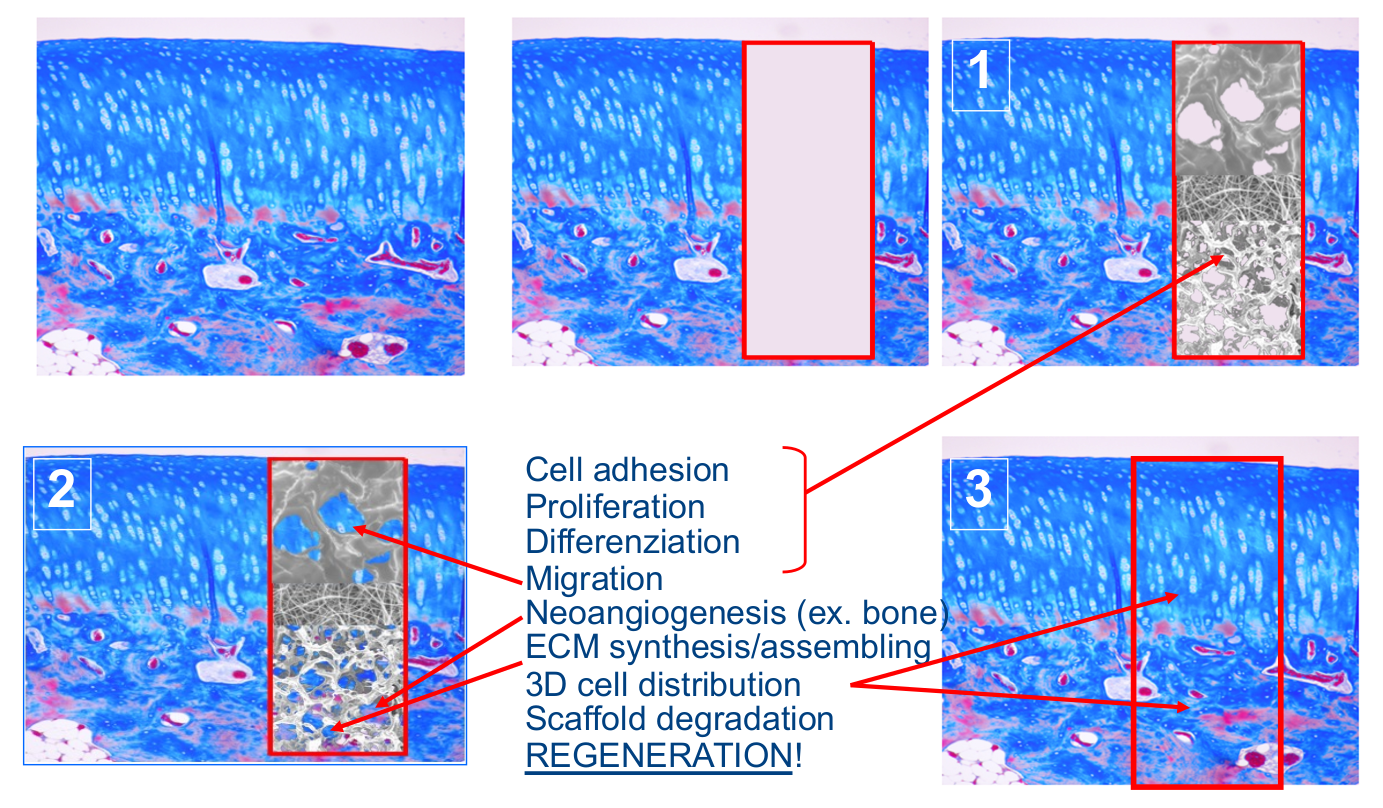
\includegraphics[width=0.5\textwidth]{cartilage.png}
			\caption{Cartilage regeneration}
			\label{fig:cartilage}
		\end{figure}

	In figure \ref{fig:cartilage} we can see an articular cartilage, an intermidiate tissue and bone.
	These three different tissues present differences in vascularization, cell organization (in cartilage cells live in lacuna, where migration and proliferation are downregulated) and innervation.\\
	In case of trauma most of the time the damage reaches the bone to the lack of innervation in the cartilage.
	Because of this a multicomponent scaffold that accounts for different types of tissues is designed.
	In particular the scaffold should:

	\begin{multicols}{2}
		\begin{itemize}
			\item Upregulate angiogenesis in the bone and downregulate it in the cartilage.
			\item Increase the water content in cartilage so to increase its compressive capabilities through hydrophilic materials.
			\item Provide an environment for osteoblasts and lacunae for cartilage cells
			\item Provide space for nerves, vascularization and cell migration.
			\item Tissue specific degradation times.
		\end{itemize}
	\end{multicols}

	After the design biocompatibility needs to be checked: it will have an impact on cell adhesion, proliferation, differentiation and migration, on neoangiogenesis and on the regeneration of the function of the damaged tissue.

	\subsection{The principles of tissue engineering}

	\begin{figure}[ht]
		\centering
		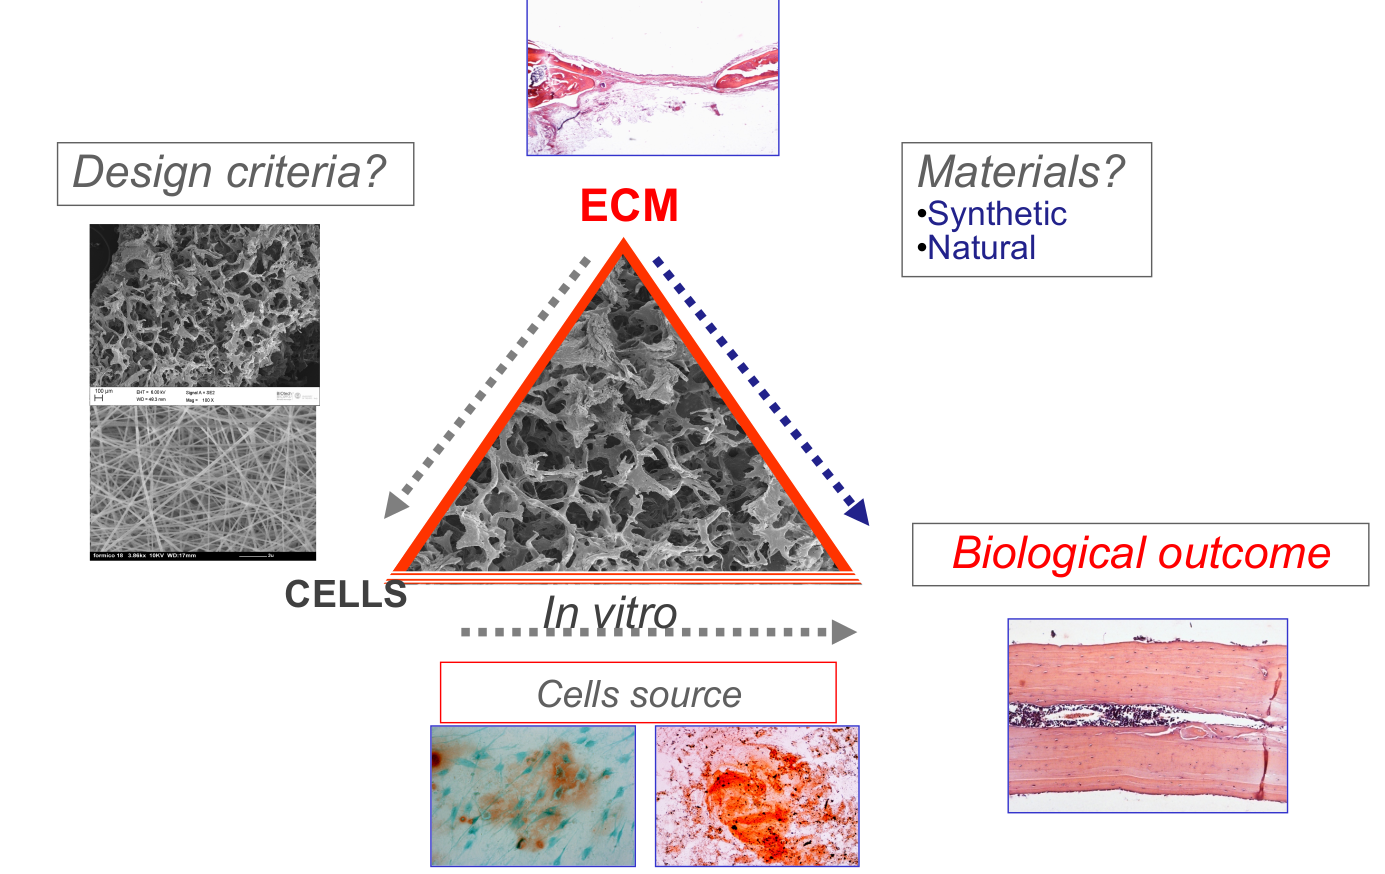
\includegraphics[width=0.5\textwidth]{triangolo.png}
		\caption{Tissue engineering principles}
		\label{fig:triangle}
	\end{figure}

	A tissue engineering process is composed by three steps:

	\begin{multicols}{3}
		\begin{itemize}
			\item Design.
			\item Material choice.
			\item In vitro and in vivo testing.
		\end{itemize}
	\end{multicols}

	Tissue engineering implements a multidisciplinary strategy and the advance in materials' science and biology drastically improve the success of scaffold application.
	The advances in biology, for example the discovery in $2000$ of macrophages \emph{M1} and \emph{M2}, allow for the design of more biocompatible scaffolds.


		\subsubsection{4th generation biological regenerative biomaterials}
		A biomaterial to be defined as a 4th generation biological regenerative biomaterial needs to:

		\begin{multicols}{2}
			\begin{itemize}
				\item Change its activity based on the environment: be, for example termo or pH responsive.
				\item Be instructional: functionalized with peptides that can control cells' fate.
				\item Have specific mechanical strength and functions to allow for mechanical signalling.
			\end{itemize}
		\end{multicols}

	Biomaterial need to be stable and inert in the beginning to allow for drug delivery, for printing organ and for cell therapies.
	The hope for the future is to develop also diagnostic systems and to implant electronic devices.

\section{Definition}

	\subsection{First definition}
	At first a material was defined as biocompatible when inert, presenting a total absence of interaction between the material and the tissues.
	Minimal reaction to the foreign body was preferred, meaning no (or low) inflammatory reaction and no immuno-response.
	This definition focuses on the body reaction to the implant, requiring on the latter only chemical stability.

		\subsubsection{Problem with the first definition - heart valves}

		\begin{figure}[ht]
			\centering
			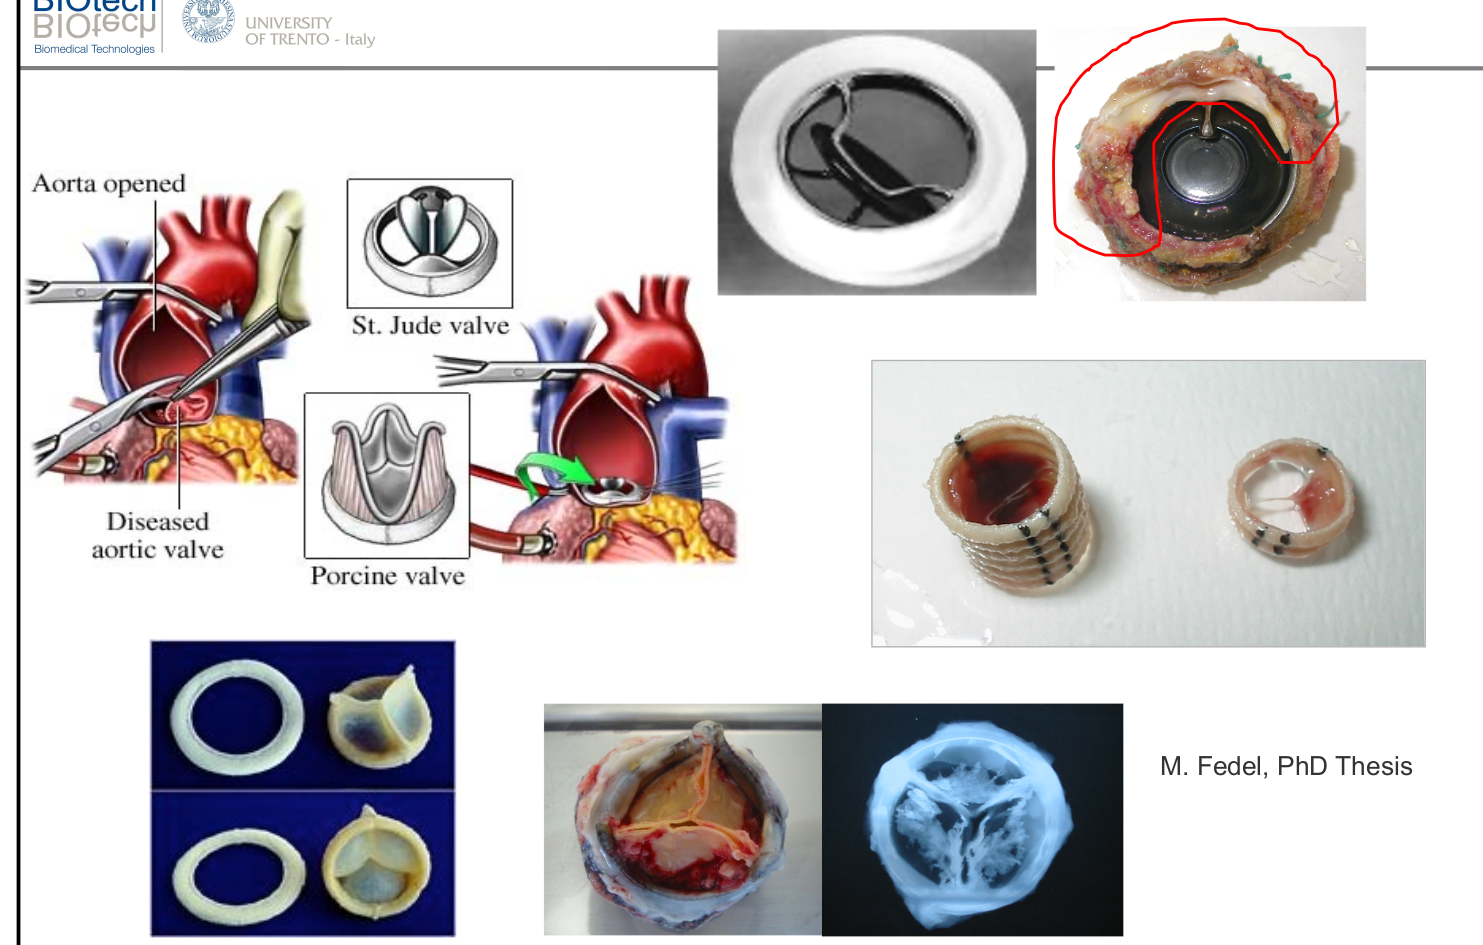
\includegraphics[width=0.5\textwidth]{valves.png}
			\caption{\label{fig:valves}}
		\end{figure}

		The problem with this definition were brought to light when observing the implant some time after the implantation.
		We will now discuss as an example the problem with heart valves.
		An heart valve made of titanium and polyester failed because around the plastic layer the body built a very thick scar tissue, not letting it open anymore.
		The same valve with an ultrathin silver layer used for antibiotic purposes caused thrombosis in other patients.
		To tackle this problem this valve was treated with anticoagulants.
		A biological heart valve harvested from pigs failed because of calcification which rendered the valve unable to close.

	\subsection{Second definition}
	All the material induce a biological reaction.
	No material is completely inert, because our antibodies can recognize anything that is not "self".
	The concept of biocompatibility was revised as the ability of a material to perform a specific application causing an appropriate host response in a specific application (1987).
	It is clear how the context of implantation is fundamental: scaffolds should be tissue and organ dependant, resolving a defined situation by reacting with the tissue and activating the cellular function to heal a specific environment, before being degraded.

		\subsubsection{FBRx - an example}

		\begin{figure}[ht]
			\centering
			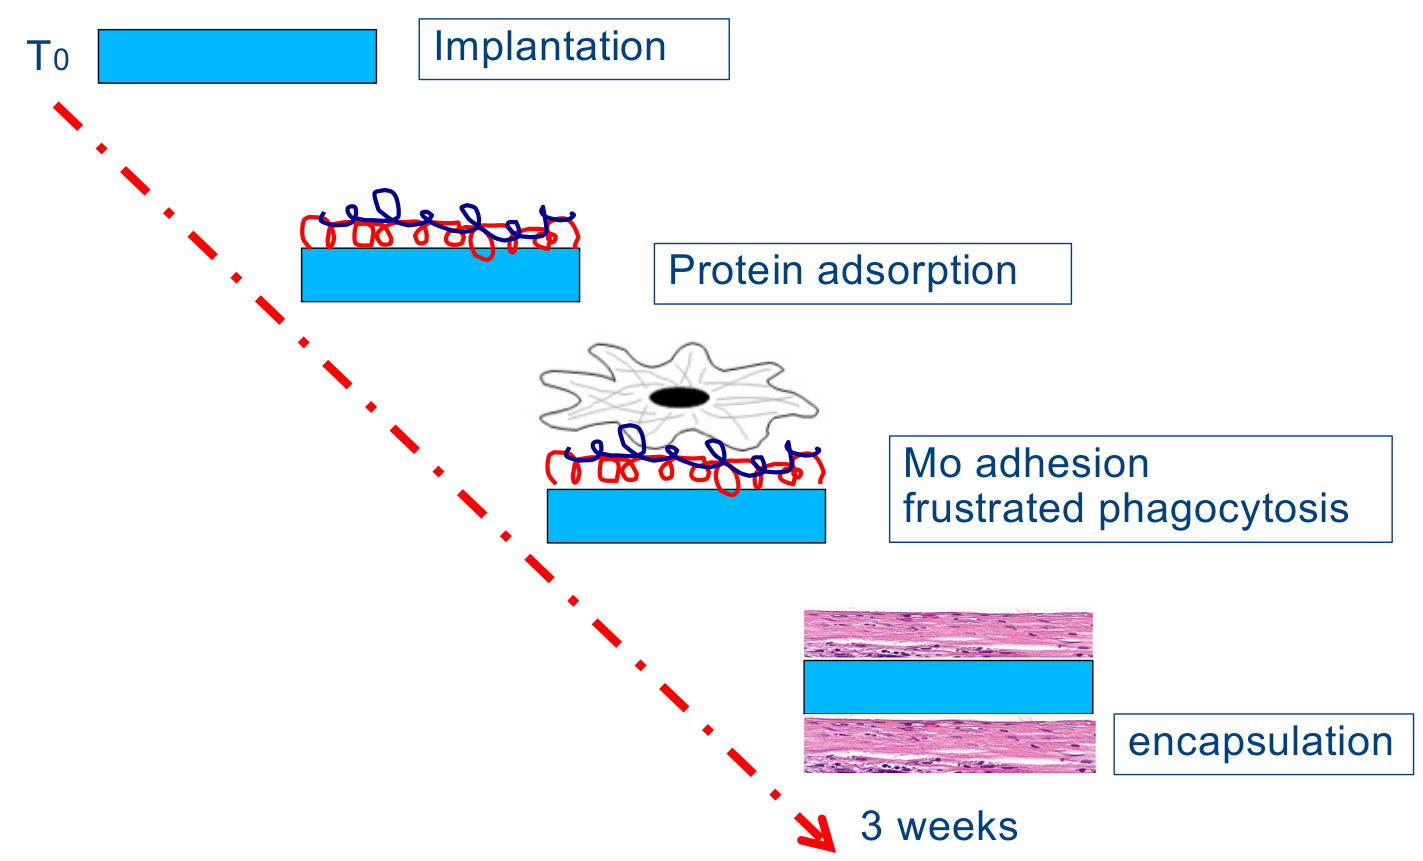
\includegraphics[width=0.5\textwidth]{fbrx.png}
			\caption{\label{fig:matrixome}}
		\end{figure}

		We can take as an example FBRx, a non porous scaffold material.
		Depending on the chemistry of the material activates a specific protein adsorption and subsequently a specific immune response.
		If the material is not degradable, the macrophages start to coat the foreign body with scar tissue, ending the adsorption reaction, allowing the scaffold to degrade, leaving an empty bag of scar tissue.
		Changing the porosity the scar tissue is reduced and regeneration is promoted.
		For this case injectable gels (hydrogel) are useful scaffold: they are porous and leave space for cell migration.
		Because of this they are used when filling cavities.

	\subsection{Re-evaluation of the biocompatibility concept}
	Some factors led to the redefinition of the concept of biocompatibiliy, as for the scaffold is not enough to simply exist.

	\begin{multicols}{2}
		\begin{itemize}
			\item Response to specific materials could vary from one application site to another, it is tissue-organ dependent: there is a need to define both material characteristics and implantation context, composed by the tissue and the injury.
			\item An increasing number of applications require that the material specifically react with the tissues rather than be ignored by them.
			\item Some applications require that the material degrade over time in the body rather than remaining indefinitely in it.
		\end{itemize}
	\end{multicols}

	Because of this biocompatibility can be considered a system's property: it cannot be defined without considering the implantation context: it involves the separate, but interrelated, responses of the two phases of the biomaterial-tissue complex and interfacial phenomena triggered by their compact.
	The key to understand biocompatibility is:

	\begin{multicols}{2}
		\begin{itemize}
			\item The determination of which chemical, biochemical, physiological, physical or other mechanism become operative and why.
			\item The determination of the highly specific conditions associated with contact between biomaterials and tissue of the body.
			\item What are the consequences of these interactions.
		\end{itemize}
	\end{multicols}

		\subsubsection{Mechanotransduction}
		Mechantransduction describes the processes at a cellular and molecular level that are involved with the transduction of mechanical stimuli into biochemical signals: structural and hemodynamic forces are encountered at the interface between tissue and scaffold.
		There will be a mismatch of elastic moduli between tissues and engineering material, causing differential stresses and strain.
		These processes will cause sensing and signalling processes to modulate gene and protein experssion profiles.

		\subsubsection{Sterile inflammation}
		Sterile inflammation is an inflammation that results from trauma or chemically-induced injury without the involvement of any microorganism.
		It si associated with the recruitment of netruphils and macrophages and the generation of pro-inflammatory chemokines and cytokines.
		The progress of biomaterial-induced sterile inflammation has to be considered during implantaion.
		Among the processes involved into sterile inflammatory response there is:

		\begin{multicols}{2}
			\begin{itemize}
				\item Pattern recognition receptros can sens conserved structural entities in microorganism and exogenous molecules.
				\item Inflammosome activated by immune system molecules induce inflammation in response to pathogens and molecules derived from the host.
				\item Marcophages change phenotype according to the stress factors from anti to pro inflammatory situations depending on the damage associated molecular patterns.
			\end{itemize}
		\end{multicols}

	\subsection{The generic biocompatibility pathway}

	\begin{figure}[ht]
		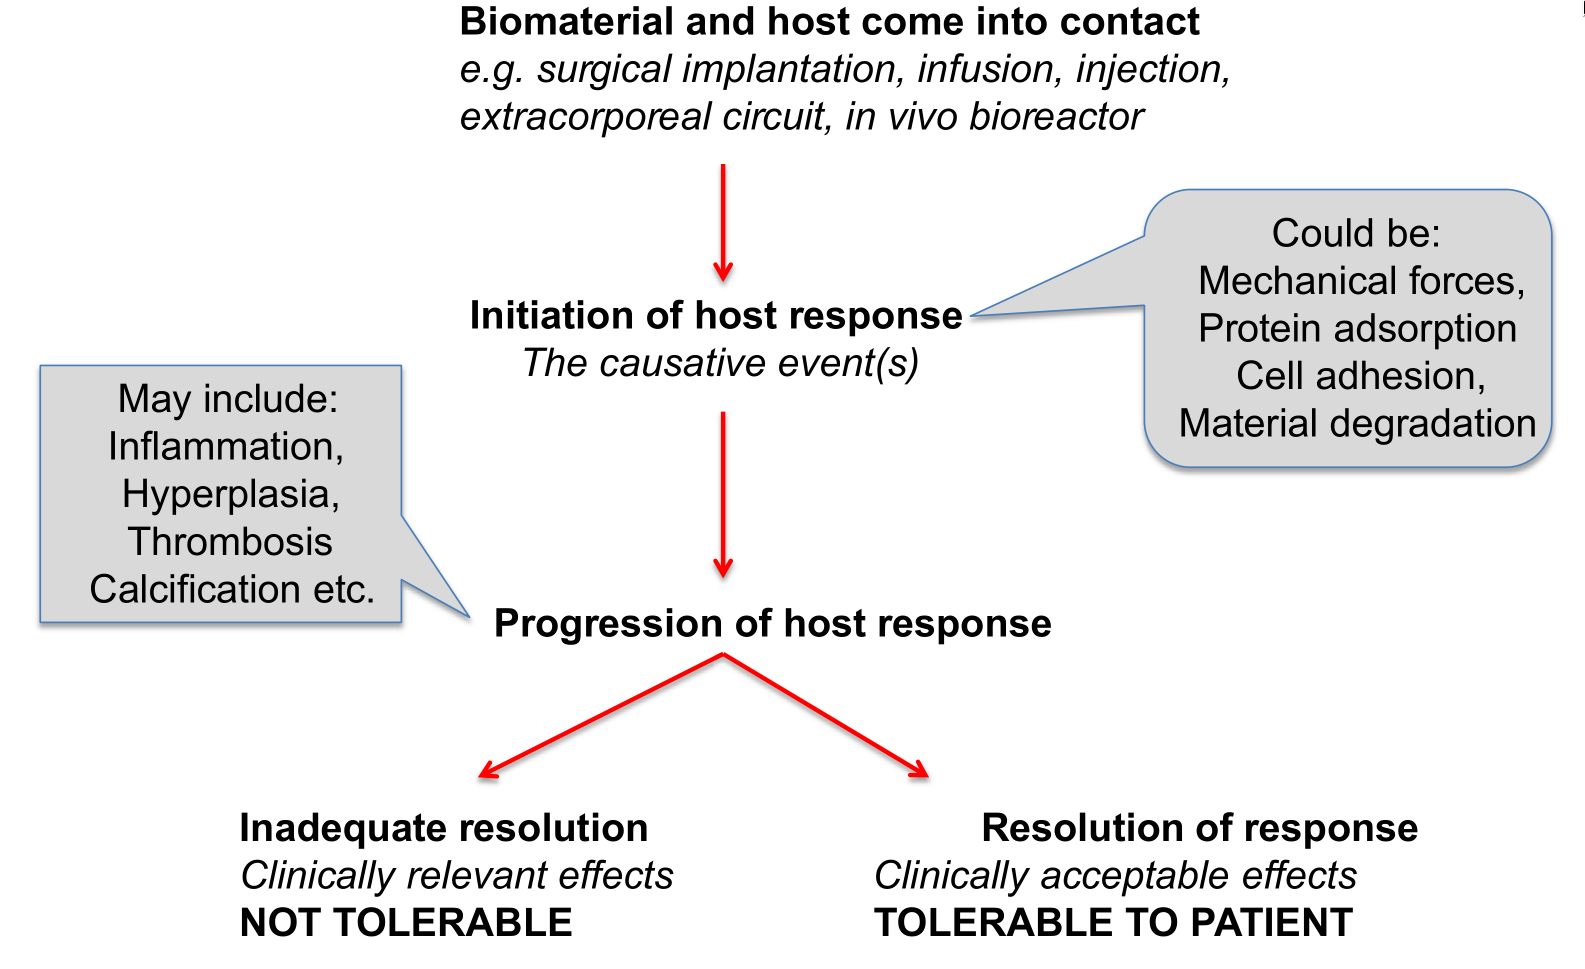
\includegraphics[width=\textwidth]{biocomp_pathway.png}
		\caption{General biocompatibility pahtway}
		\label{fig:biocomp_path}
	\end{figure}

	The simple generic pathway (figure \ref{fig:biocomp_path}) starts with the presentation of a clinical condition which leads to the decision to use a biomaterials-based therapy.
	The biomaterial may interact with cells in the determination of the appropriate host response.
	In most situations the desired clinical outcome can only be achieved through a combination of effects on critical cells and the avoidance of effects on other cells.
	The part of the pathway between biomaterials and cells constitutes the generic biocompatibility pathway.
	The biomaterial will influence the events through mechanical or molecular signalling processes.

		\subsubsection{Cells}

		\begin{figure}[ht]
			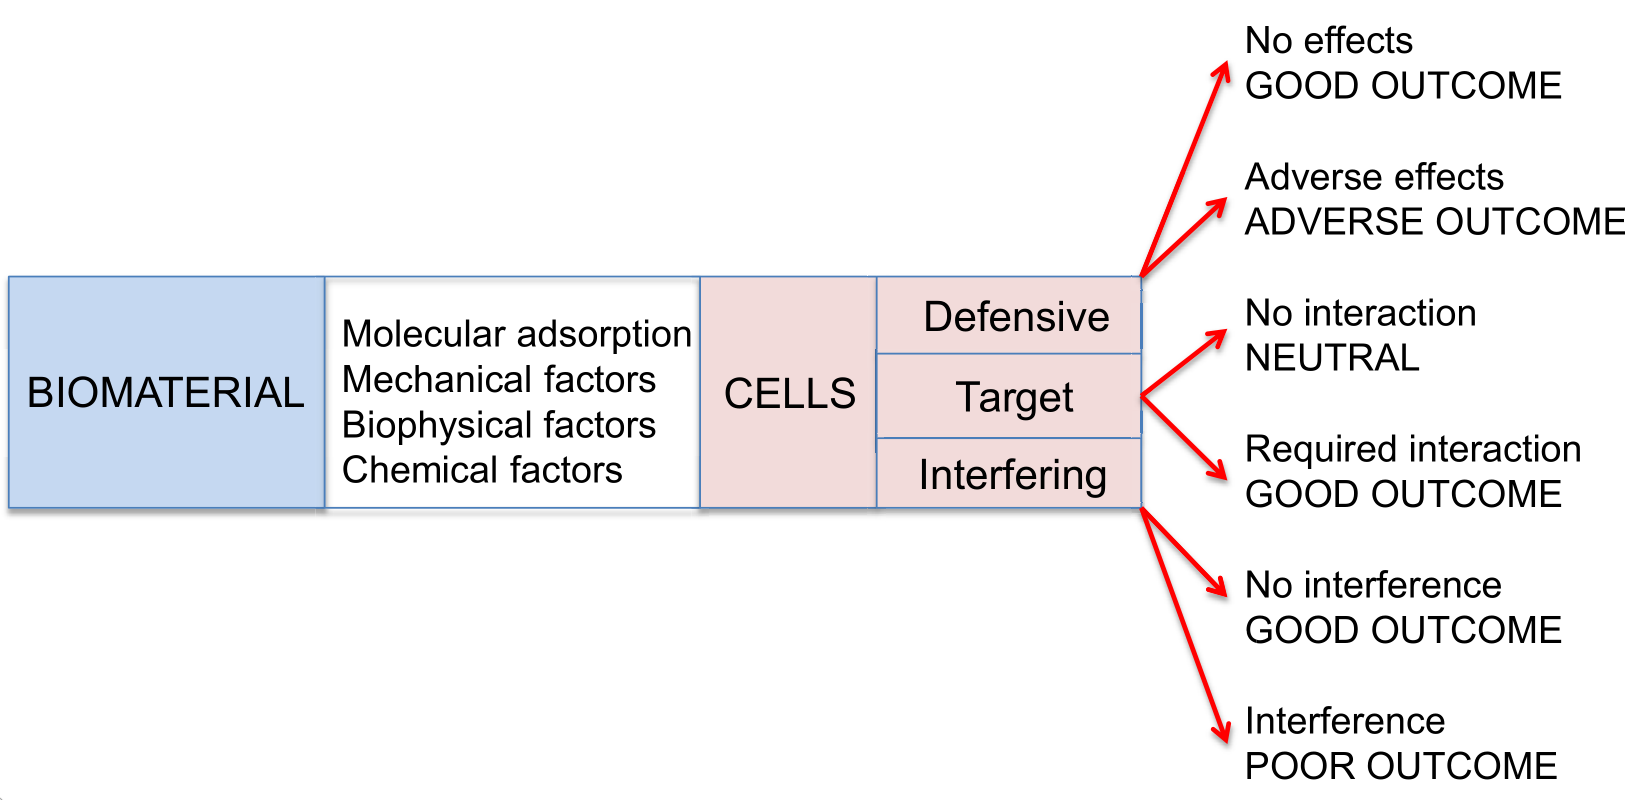
\includegraphics[width=\textwidth]{biocomp_cells.png}
			\caption{Cells involved in a general biocompatibility pahtway}
			\label{fig:biocomp_cells}
		\end{figure}

		Cells on this framework (figure \ref{fig:biocomp_cells}) can be:

		\begin{multicols}{2}
			\begin{itemize}
				\item Target cells: cells at which the therapy is aimed.
				\item Defensive cells: cells of innate and adaptive immunity, whose job is to repel and remove injurious external agents.
				\item Interfering cells: cells that interfere with the response that the biomaterial is seeking.
			\end{itemize}
		\end{multicols}

		The biocompatibility pathway will be determined by the events in these groups.
		The key to an appropriate host response is the dominance of the desirable effects over undesirable effects on the target cells, coupled with the avoidance of unacceptable responses via the defensive and interfering cells.
		The effects of chemical and mechanical events mediated by the biomaterial on cells are described on figure \ref{fig:biocomp:chem}


		\begin{figure}[ht]
			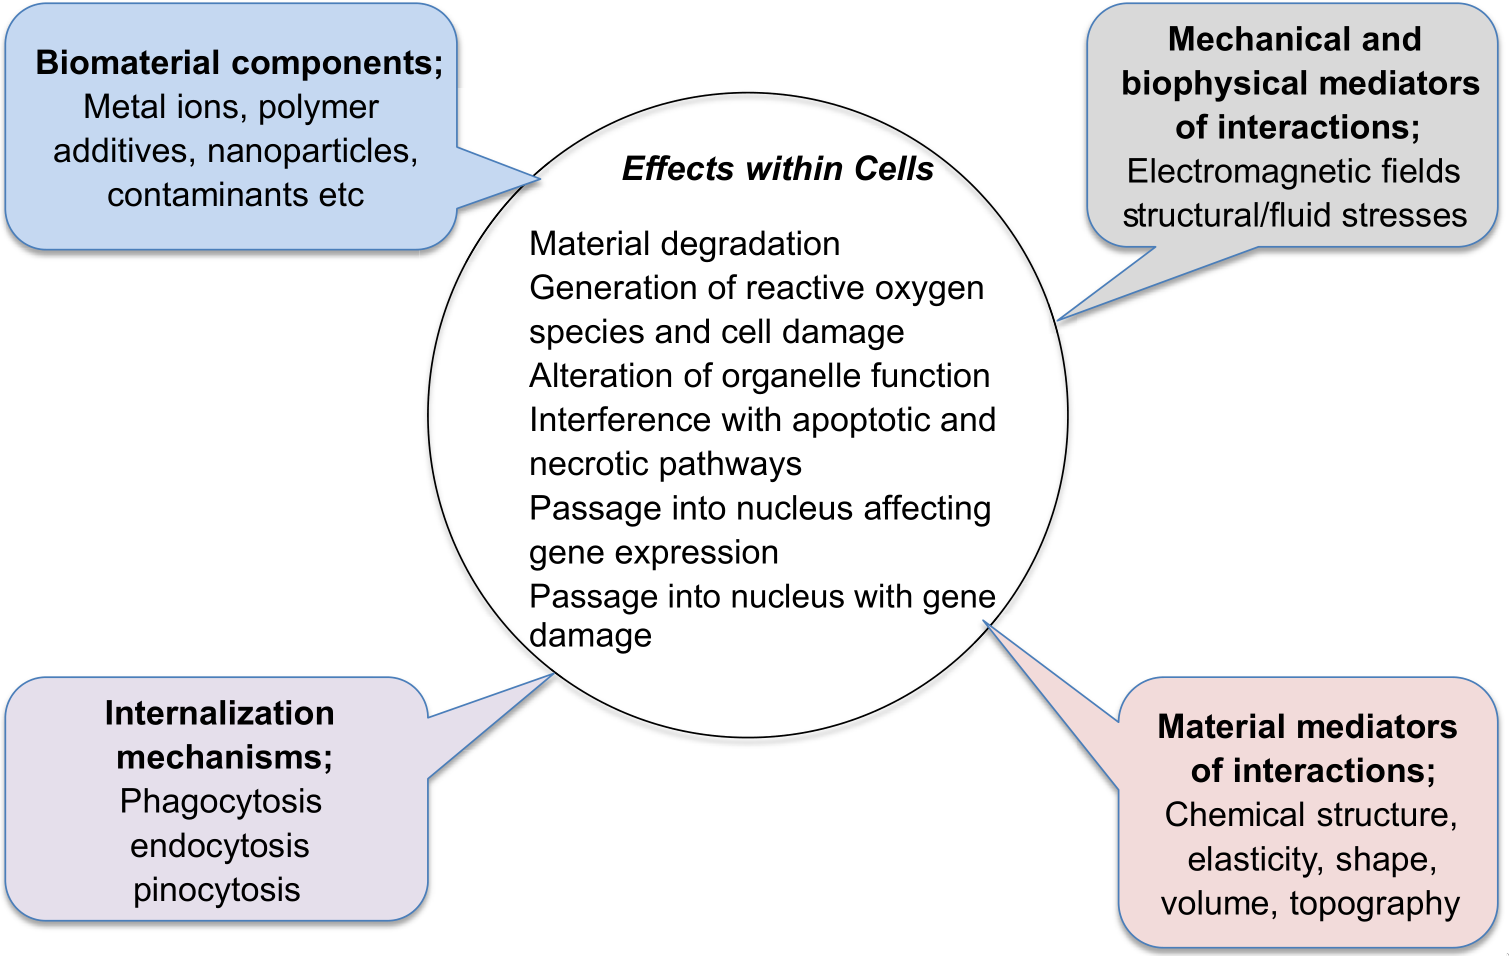
\includegraphics[width=\textwidth]{biocomp_chem.png}
			\caption{Effects of biomaterial-mediated events on cells}
			\label{fig:biocomp_chem}
		\end{figure}

\section{The complexity of the biocompatible system}

\begin{figure}[ht]
	\centering
	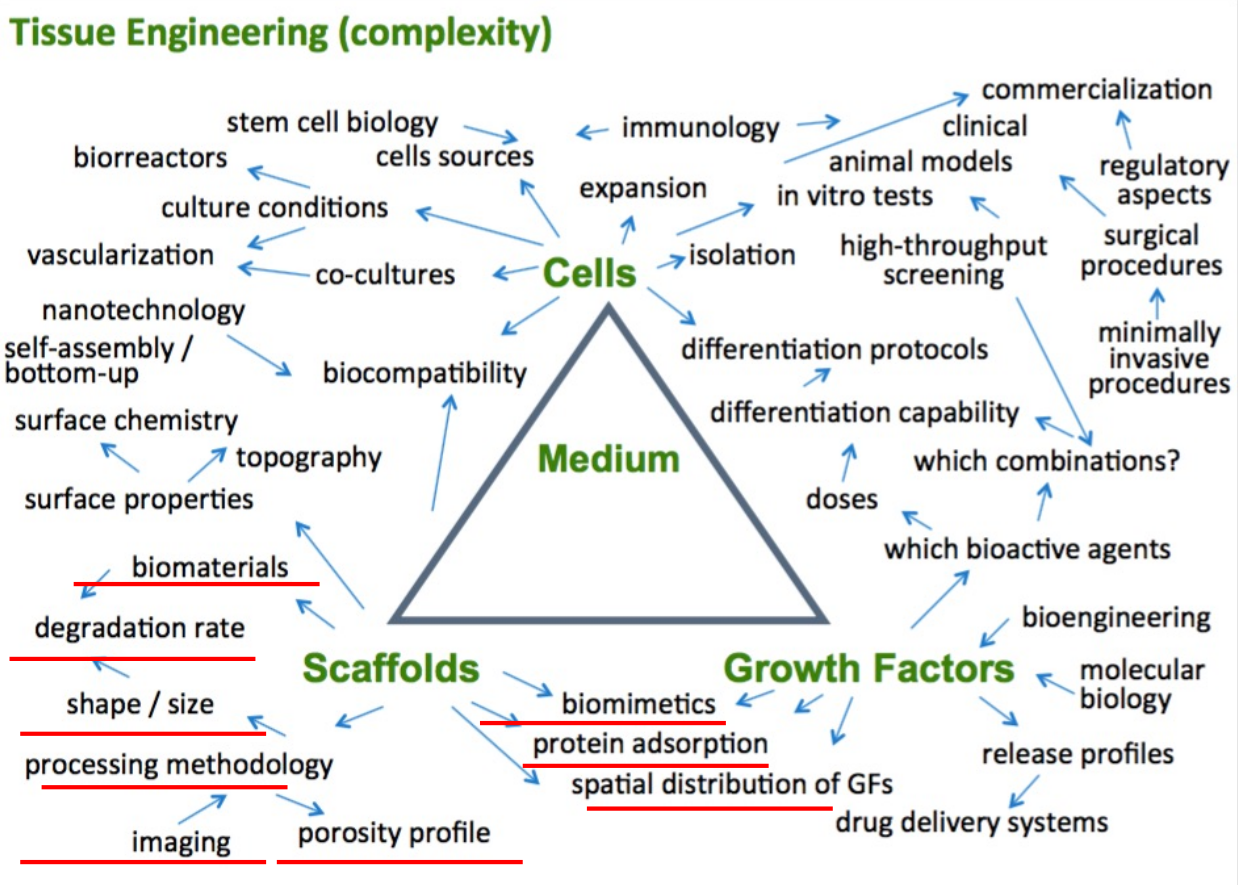
\includegraphics[width=0.8\textwidth]{piramide_completa.png}
	\caption{Tissue engineering can be represented considering three actors\label{fig:complete_pyramid}}
\end{figure}

As can be seen in figure \ref{fig:complete_pyramid} only three actors are present in the tissue engineering paradigma, but each one has many ramification and possibilities.
\\
To design a biocompatible scaffold there is a need to take into account:

\begin{multicols}{2}
	\begin{itemize}
		\item Determination of native tissue or organ context.
		\item In vivo testing with bioreactors that provide a dynamic environment and can provide mechanical stimuli by perfusion.
		\item Passage from in vitro to in vivo testing selecting an appropriate animal model.
		\item Definition of the surgical model and finally we move to clinical trials.
	\end{itemize}
\end{multicols}

	\subsection{ECM molecules production: effect of the mechanical stimuli on a cartilage scaffold}

	\begin{figure}[ht]
		\centering
		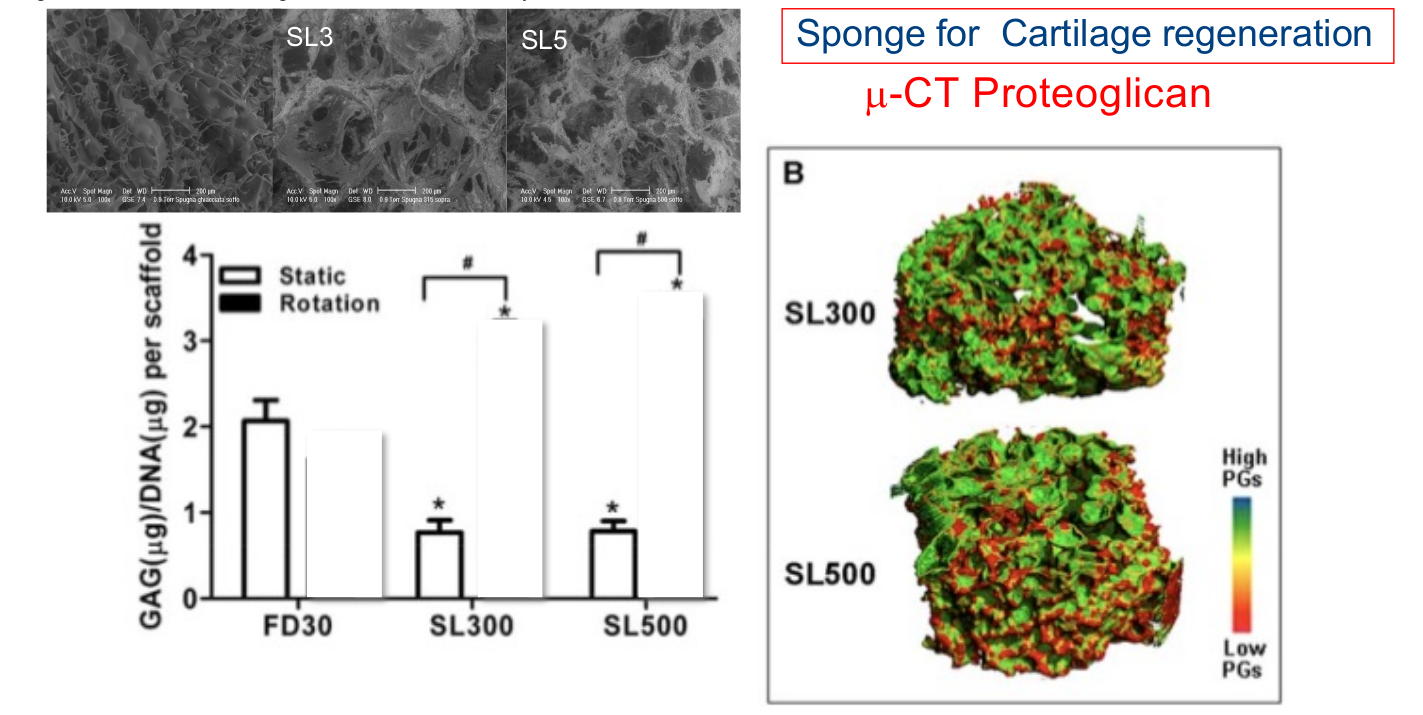
\includegraphics[width=0.5\textwidth]{sponge.png}
		\caption{Cartilage sponges' quality assessment}
		\label{fig:matrixome}
	\end{figure}

	Different sponge-like scaffolds were produced with different properties like porosity for cartilage regeneration.
	The quality of GAG (glycosamminoglycans) mainly into the ECM of cartilage was assessed.
	In addition microCT, a 3D imaging technique was used to see the level of infiltration of GAGs into the sponges.
	It can be seen in image \ref{fig:matrixome} how SL500 had a lot of green, representing GAG, but only on the outside of the sponge.
	When the sponges undergo a mechanical stress similar to the biological situation the infiltration was present also in the inside of them.
	So, changing from a static to a perfusion environment the behaviour of the molecules and the sponges changed drastically.
	In particular during perfusion integrins were upregulated.
	This molecules are transmembrane proteins responsible for cell to cell and cell to extracellular matrix communication and imparted an instructive behaviour to the cells, which are extremely sensible to it.

    \graphicspath{{chapters/03/images/}}
\chapter{Extracellular matrix - ECM}

\section{Introduction}

	\subsection{ECM functional role}
	The extracellular matrix provides a starting point for scaffold biodesign in tissue engineering.
	It is a dynamic environment produced and regulated by cells which performs different functions:

	\begin{multicols}{2}
		\begin{itemize}
			\item Aids in cell locomotion through transmembrane receptors and ligands in the ECM.
				This adhesion ligands are patterned in order to direct cell locomotion in a specific direction.
			\item Transmits and distributes mechanical loads: the ECM assumes a specific structure in order to transmit mechanical stresses to the cell in a tissue-specific manner.
			\item Prevents premature mechanical failure.
			\item Partitions cells and tissues into functional units.
			\item Acts as a scaffold defining tissue and organ architecture.
			\item Acts as a storage and dissipative device for elastic energy.
			\item Acts as substrate for cell adhesion, growth, and differentiation.
				Adhesion is the activation step that allows for cell growth and differentiation, and because of this it fundamental for the activation of regenerating cells.
		\end{itemize}
	\end{multicols}

	The ECM is a controlled complex network composed of proteins, glycoproteins and proteoglycans (PGs), which assemble in a tissue-specific manner to provide tissue specific biophysical and biochemical properties.

		\subsubsection{ECM-cell interaction}
		The interaction of the ECM with the cells is necessary as to avoid cells entering into a pathogenic state.
		Cell's nuclei and the ECM interact through integrins.
		This integrins convert external signals into a context-specific gene expression profile.
		The ability of cells to sense the chemical, mechanical and topographical features of the ECM enables them to integrate complex, multiparametric information into a coherent response to the surrounding microenvironment.
		Consequently, dysregulation or mutation of ECM components results in a broad range of pathological conditions.
		Because of this the ECM can be considered as a composite material where cells sense the environment.
		ECM polymers or networks are instructive: they provide structural and mechanical integrity to tissues.
		A tissue engineering scaffold should activate this integrins and ligands as to activate the gene expression profile necessary for regeneration.
		The focus should be on activating the correct pathway as to have the desired therapeutic effect and not a damage one.

		\subsubsection{Regulating cells' fate}
		The ECM controls whether a cell should undergo apoptosis or necrosis.
		Apoptosis is a programmed cell death, in which cells are encapsulated by vesicles and removed.
		Necrosis instead happens when the cellular membrane is damaged, causing the rupture of the cell and inflammation.
		During necrosis the activity of macrophages is increased, producing also inflammation for neighbouring cells.
		It has been suggested to induce tumour cell death through apoptosis to avoid upregulating inflammation.

	\subsection{Components of the ECM}
	The ECM is composed of different molecules:

	\begin{multicols}{2}
		\begin{itemize}
			\item Physical signals: fibronectin, vitronectin, collagen, laminin, fibrillin, glycosamminoglycans (GAGs), PGs.
			\item Soluble signals: growth factors (GF), cytokines, chemokines, used for communicating with distant cells.
			\item Structure: fiber-based and function dependent composites.
			\item Water: tune mechanical properties to better support compressive stress.
				Highly present in articular cartilage, its content is controlled by GAGs and PGs.
			\item Mechano-transduction: translating mechanical stimuli.
		\end{itemize}
	\end{multicols}

		\subsubsection{Collagen fibers}
		The ECM is composed mostly of collagen fibres, which can be organized into:

		\begin{multicols}{2}
			\begin{itemize}
				\item Fibrils, very elastic structures.
				\item Fibres: more thicker and stiff than fibrils.
				\item Bundles: composition of bundled fibres.
			\end{itemize}
		\end{multicols}

		To better tune the mechanical properties without changing the ECM's chemistry the orientation of the fibres will change, depending on the external mechanical stimuli.
		Change the organization of the fibres cause modifications in water content and rigidity, causing a completely different signal to be sent to the cells communicating with the ECM.

		\subsubsection{Signals}
		Signals are fundamental for cell adhesion and must be considered when designing a scaffold together with ligands and collagen.
		To reduce scaffold complexity by decreasing the number of molecule necessary in a scaffold multifunctional polymers are being developed.
		The cross-talk between cells and the ECM allows for the control of many processes like:

		\begin{multicols}{3}
			\begin{itemize}
				\item Pattern formation.
				\item Morphogenesis.
				\item Cell fate.
				\item Daily cellular processes.
				\item Wound healing.
				\item Tissue homeostasis.
			\end{itemize}
		\end{multicols}

		\subsubsection{Stem cells}
		Stem cells are uniquely capable of reproducing themselves through self-renewing and of differentiating into the different cell types necessary to perform a specialized function.
		They are fundamental in embryogenesis and a control between self-renewal and differentiation is fundamental in the healing process and homeostasis.
		Deregulating this process can cause tumorigenesis, degeneration or a pathogenic state.
		Because of this they are very sensible to the ECM and to the environment.

\section{The matrixome: chemistry of the ECM}

\begin{figure}[ht]
	\centering
	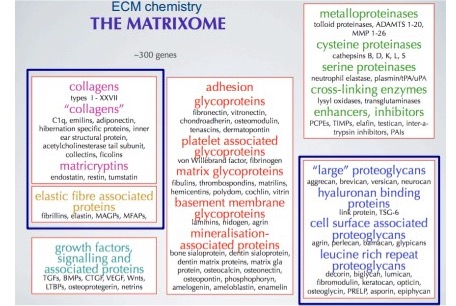
\includegraphics[width=0.8\textwidth]{matrixome}
	\caption{ECM content}
	\label{fig:matrixome}
\end{figure}

The ECM is a mosaic structure that guides cell differentiation and function.
It is a composite material that comprises a fibrous structural net embedded in a porous hydrated gel matrix of GAGs.
Different properties of the ECM are controlled by different molecules, depicted in figure \ref{fig:matrixome}, present in it:

\begin{multicols}{2}
	\begin{itemize}
		\item Stiffness: collagens.
		\item Elasticity: elastic fibres.
		\item Cell-cell communications: signalling molecules like growth factors.
		\item Cell adhesion and mobility direction: adhesion molecules.
		\item Dynamic response: proteinases, which can be used to degrade the scaffold once it is no more needed.
		\item Water content: GAGs and PGs.
	\end{itemize}
\end{multicols}

	\subsection{ECM - cell interaction}
	The cellular membrane is rich in proteins able to sense the external environment and transfer the information to the nucleus, activating a specific gene expression.
	When designing a scaffold, one must provide it the ability to interact with cells with an appropriate mechanism as not to deregulate cellular and tissue mechanisms.

	\begin{figure}[ht]
	\centering
	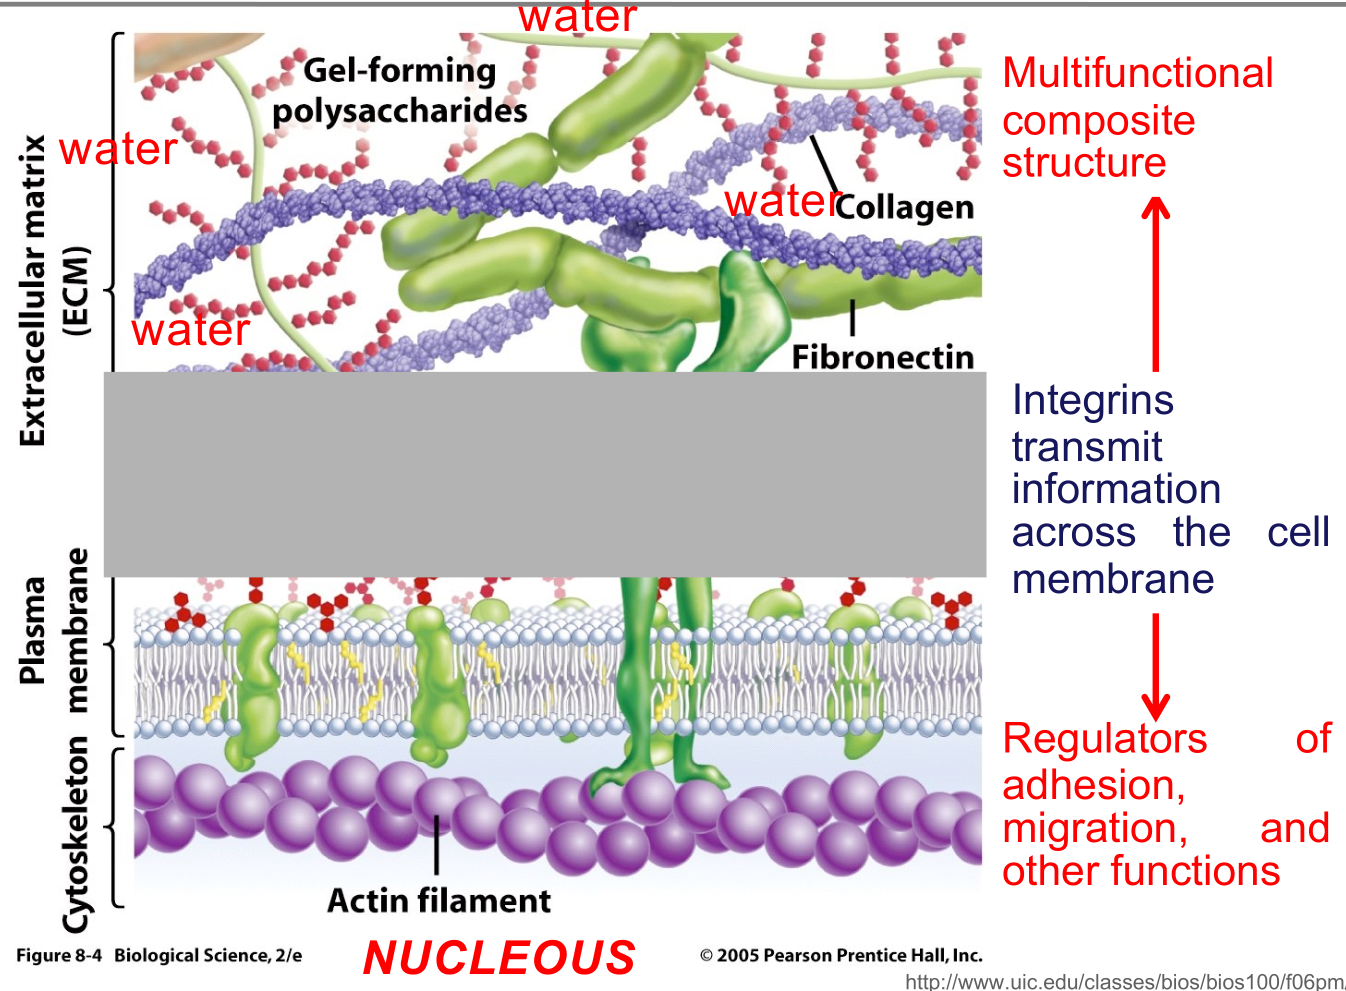
\includegraphics[width=0.6\textwidth]{structure}
	\caption{\label{fig:structure}}
	\end{figure}

	The ECM is a mosaic structure, a guide for cell functions.
	Natural ECM modulate tissue dynamics through their ability to locally bind, store and release soluble bioactive ECM effectors.


	\subsection{Matricellular proteins}
	Matricellular proteins are extracellular modulators of cell function expressed at high level during development and in response to injury.
	They are modulators of cell matrix interactions and bind to many cell surface receptors and to the ECM GFs.
	They are cytokines and proteases.
	Their role is to induce de-adhesion in contrast to the adhesivity of most matrix proteins allowing for cell migration.
	Other functions are:

	\begin{multicols}{2}
		\begin{itemize}
			\item Cell adhesion, migration, chemotaxis.
			\item Matrix assembly and collagen fibrillogenesis, helped through some factors like ascorbate.
			\item Regulation proliferation/apoptosis.
			\item Binding/activation GFs and cytokines.
			\item Angiogenesis and tumour growth.
		\end{itemize}
	\end{multicols}

	For example, TSP1 and 2, Tenascon-C and SPARC support a state of intermediate adhesion, with disruption of focal adhesion and the reorganization of actin stress fibres.

	\subsection{Collagen}
	Collagen is one of the most important proteins for the ECM, as it provides structural properties.
	In the ECM collagen assembles into fibrils, then fibres and bundles when needed.
	Collagen is a family of proteins with at least 23 different types.
	Depending on the tissue, there is a prevalence of one type on others.
	In the cartilage for example type II collagen is the most represented, while in tendons it is type III collagen, which is really similar to jellyfish collagen, currently commercialized.

		\subsubsection{Different collagen structures}
		The collagen can assemble in different structure, granting different mechanical properties to the ECM.
		For example:

		\begin{multicols}{2}
			\begin{itemize}
				\item Connective tissue: less density, soft network, more water, fiber and fibrils.
				\item Meniscus: parallel fibers, more density, packed fibers, because of different functions, bundle (more stress).
				\item Myocardium: mechanical stresses, it should support the growth in one direction.
			\end{itemize}
		\end{multicols}

		\subsubsection{Cell-collagen interaction}
		Cells can migrate in a collagen low porosity material through a specific enzymatic process, which allows the opening of the collagen structure.
		A scaffold should be designed to promote cell migration.

		\subsubsection{Chemical characteristics and synthesis}
		Collagen is non-homogeneous, bottom-up, multi-functional, dynamic and has a hierarchical structure which is function dependent.
		It is composed by three chains that can form an helix formation.
		Controlling the chemical bridges between the chains the elasticity of collagen can be changed.
		Collagen production starts in the cell, where it is synthesized.
		Then selected prolines and lysines in it are hydrolysed.
		Later the hydrolysines are glycosylated, and three $\alpha$-chain assemble, forming the procollagen triple-helix.
		This triple helix is secreted.
		In the ECM the propeptides are cleaved and the resulting collagen molecules can self-assembly into fibrils.

		\subsubsection{Dynamic nature of the ECM}
		The ECM is degraded by cell-secreted proteases and releasing bioactive components that remodel the collagen structure.
		Natural ECMs modulate tissue dynamics through their ability to locally bind, store and release soluble bioactive ECM effectors such as GFs.

	\subsection{Fibronectin}
	Fibronectin is a large matrix glycoprotein present in most body tissues' fluids.
	Functionally, it is the classic example of an adhesive glycoprotein, binding and interconnecting extracellular matrix components with each other and to the surface of the cells.
	It is one of the most important molecules through which cells interact with the surrounding environment.
	The binding of fibronectin to the cell surface’s integrin receptors plays a critical role in cell migration during the development and postnatally.
	It also plays a role as chemo-attractant for cells in a damage site.
	Its fragments after a damage promote wound contraction.


		\subsubsection{Chemical characteristics}
	Fibronectin is a dimer composed of two identical chains connected by a disulphide bond.
	Different sections of fibronectin can be recognized:

	\begin{multicols}{2}
		\begin{itemize}
			\item One can interact with fibrin and heparin.
			\item One can interact with gelatine and collagen.
			\item One can interact with the cell receptors through the arg-gly-asp ac. sequence.
			\item One can interact with the polysaccharide heparin.
			\item One can interact with fibrin.
		\end{itemize}
	\end{multicols}

		\subsubsection{Fibronectin interaction}
		Fibronectin is able to interact and crosslink different molecules as to transmit signals and stimuli in the ECM.
		This allows cells to respond quickly to changes in the environment.
		The RGD-loop in fibronectin is strategically placed to undergo strong conformational changes and constitutes a mechanosensitive switch for recognition by integrin receptors.
		Depending on the mechanical stimulus, fibronectin can assume specific conformations, changing its activity and, in doing so, changing the signal that it sends.
	In ECM we have fibronectins, collagen, gel-forming polysaccharides, water, actin and the cell (figure \ref{fig:structure}).

	\subsection{Proteoglycans and GAGs}
	Proteoglycans are composed of a head core protein and a chain of polysaccharides, which is hydrophilic (figure \ref{fig:pgag}).
	The chain of polysaccharides is composed of glycosamminoglycans or GAGs, long linear polysaccharides consisting of repeating disaccharide units, composed of a uronic sugar and an amino sugar, which is usually sulfated.
	Proteoglycans are responsible for controlling the water content of the tissue.
	They aid the ECM in responding do mechanical stresses.
	Many proteoglycans can be linked together via long hyaluronic acid chains, forming giant complexes.
	In the cartilage matrix, for example, individual proteoglycans are linked to a non-sulfated GAG: hyaluronic acid to form a giant complex.
	Hyaluronic acid in particular creates cell-free space during embryogenesis filled with water into which cells can proliferate and migrate.
	Because of their negative charges, glycosaminoglycans and proteoglycans together control the water content of the tissue, determining the degree of ”squishiness” of the matrix.
	They also allow for $H_2O$ reentry after tissue compression.
	In fact, during compression, water gets squeezed out and the negative charges of PGs and GAGs draw Na ions, creating an osmotic pressure and forcing the escaped water back in when the compression force is no longer in place.

	\begin{figure}[ht]
		\centering
		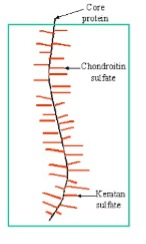
\includegraphics[width=0.3\textwidth]{pgag}
		\caption{\label{fig:pgag}}
	\end{figure}


		\subsubsection{Core protein}
		Glycosaminoglycans are linked to a core proteins in proteoglycans.
		This core protein can be:

		\begin{multicols}{2}
			\begin{itemize}
				\item Hyaluronic acid.
				\item Chondroitin sulfate.
				\item Keratan sulfate.
			\end{itemize}
		\end{multicols}

		The core protein, which is hydrophobic is usually surrounded with hydrophilic molecules.

		\subsection{Elastin}
		ECM flexibility and extensibility are due to a network structure composed of elastin, a fibrillar protein that consists of $36$ domains.
		This protein has alternating hydrophobic and crosslinks domain responsible for the long-range deformation of elastin and its high molecular mobility.
		It is composed during elastogenesis from the monomer tropoelastin released into the ECM.
		The interaction of elastin, that provides elasticity, and collagen, that provides stiffness, is fundamental for the mechanical properties of connective tissues.
		It can also transmit signals to the cells.

\section{Some examples of ECM function dependent organization}

	\subsection{Aorta wall}
	Considering the three main layers of aorta wall, the orientation and organization of collagen and elastin change, as structural adaptive response to mechanical requirements.

		\subsubsection{Mechanical requirements}
		Specific compliance and strength in both longitudinal and circumferential directions.

		\subsubsection{Structural strategy}
		Anisotropic and elastic multi-layers laminate, different fibre orientation through the thickness of the aorta wall.

		\subsubsection{ECM main components}
		A 3D fibrous network of collagen combined with elastic fibres.

		\subsubsection{Sub-endothelium}
		Multilayered fabric of collagen.
		In a layer collagen fibres are uniformly oriented, while in different layers they have a different orientation to ensure proper resistance.
		Elastin is arranged following a 3D network of elastic fibres.

		\subsubsection{Media}
		The media consist of a complex network of smooth muscle cells, elastin and bundles of collagen fibrils.
		The fenestrated elastic laminae separate the media into several concentrically fibre-reinforced medial layers.
		This form alternating layers called musculoelasic fascicles.
		It is separated from the intima and the adventitia by internal and external elastic lamina, with a cicunferentially oriented continuous elastin fibrous helix.
		The media can resist high loads in the circumferential direction.

		\subsubsection{Adventia}
		Collagen fibres are organized in thick bundles.

		\subsubsection{Intima}
		One layer of endotheliual cells in contact with the blood flow, supported by an elastic lamina.

	\subsection{Bone}

		\subsubsection{Mechanical requirements}
		High strength and rigidity combined with good toughness.

		\subsubsection{Structural strategy}
		In corical bone, collagen fibrils are densely packed and form concentric lamellae.
		Fibrils in adjacent lamellae are arranged in perpendicular planes.
		Trabecular bone has a loosely organized porous matrix.

		\subsubsection{Composition and structure}
		The bone main function is to sustain and protect organ in the body and act as a storage for mineral homeostasis.
		It is characterized by a unique composition which gives rigidity and strength while maintaining elasiticty.
		Minerals and collagens provide good hardness, compressive, tensile and torsion strengths.
		It contanis osteoprogenitor, osteoblasts, osteocytes and osteoclasts.
		In cortical or compact bone collagen fibrils form concentric lamellae perpendicolar in adjacent one.
		Trabecular or cancellous or spongy bone has loosely organized spongy arrangement.

	\subsection{Hyaline cartilage}

		\subsubsection{Mechanical requirements}
		Flexible tissue, but strong and resistant to high pressure.

		\subsubsection{Structural strategy}
		Biphasic poroelastic medium with a heterogeneous structure: many layer with different properties and orientation of fibers.

		\subsubsection{Gradient structure}
		Collagen fibrils in the superficial zone are parallel to the surface to provide great tensile and shear strength.
		There are three zones defined by collagen fibres orientation: in the superficial they are parallel, in the transitional random and in the radial perpendicular.
		$80\%$ of the tissue is water.


\section{Modelling nature}
When designing a scaffold the coal is to provide components that will drive tissue regeneration.
The environment in with the scaffold will be implanted is dynamic, with water allowing for most of the interactions.
These interactions regulate a lot of processes, in which there is cell fate, tissue formation and tissue regeneration.
The scaffold needs to allow the cells to work in a natural way, and because of this needs to be modelled based on what is observed in nature.
Living organisms naturally provide a multiplicity of materials, architectures, systems and functions, all resulting from a stringent selection process.
So, a strategy to design a scaffold should include:

\begin{multicols}{2}
	\begin{itemize}
		\item Polymers able to integrate.
		\item Molecular synthesis, done by the cells, at very high level of organisation, allowing molecular recognition, multifunctionality, self-diagnosis and a destruction-recycling process.
		\item Structure dynamics through responsive polymers, allowing for self-assembling, molecule interactions, adaptation and self-healing.
	\end{itemize}
\end{multicols}

The bottom-up approach is more bio-mimetic, as it reflects how nature works: self-assembling blocks, which assemble thanks to the environment to perform a function.
The scaffold design should account for building a context-specific microenvironment.

    \graphicspath{{chapters/04/images/}}
\chapter{Inflammation}

Biocompatibility is the ability of a material to perform with an appropriate host response in a specific application.
The first system interacting with the scaffold is the immune system, which first gives an immuno response and then starts the healing process.
Such system can be different tissue by tissue, from healthy or pathologic tissue, etc.
A widespread idea derived from findings in diverse species is that the loss of regenerative capacity is linked to the evolution of immune competence.
The relationship between tissue healing and the immune response is very complex, since there are both negative and positive roles, depending on the tissue, organ and life stage (embryonic, neonatal or adult). We need to try to reduce inflammation as soon as possible, in order to prioritize healing.
\\
\\
\noindent
If we have a wounded skin in a fetus we will have complete regeneration without scar tissue formation, whereas in adults we observe fibrotic healing. We can take some parameters from the fetal model to try to reduce as much as possible scar tissue formation in adult patients.

\section{Tissue damage}
During the inflammatory response (defence step) we have platelet activation, coagulation, inflammation, leading to bleeding, pathogens, open wound, cell debris.
Our aim is to block the wound.
The body first triggers a coagulation cascade, then the system will be activated to regenerate.
\\
\\
\noindent
In 3-7 days we have migration, proliferation, synthesis, angiogenesis.
For pathogens we need scar tissue blocking the entrance; inside pathogens need to be addressed by internal inflammation, increase blood flow into the damaged site through angiogenesis (more capillaries).
The overall process is controlled by inflammatory system cells e.g. macrophages.
Cells are coordinated by interleukines e.g. IL-1, IL-2.
\noindent
What kind of cells are involved? There are three major roles of complement:
\begin{itemize}
\item opsonize particles for phagocytosis (need only reach the C3b stage). Phages can recognize the mark through integrins.
\item elicit inflammatory reaction by acting on leukocytes, mast cells, endothelium
\item complement-mediated cytolysis
\end{itemize}
\noindent
The processes are described in figure \ref{fig:roles}.

\begin{figure}[ht]
\centering
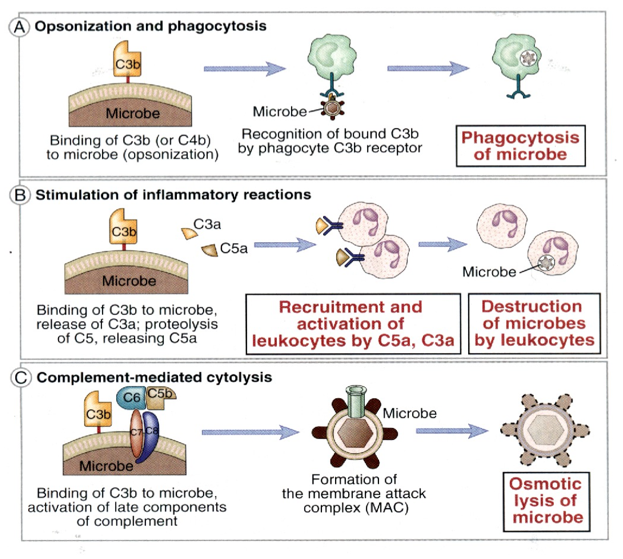
\includegraphics[width=0.6\textwidth]{roles}
\caption{\label{fig:roles}}
\end{figure}

\section{Leukocyte population}

\textbf{Neutrophils/polymorphonuclear} are the most abundant circulating leukocytes.
There are 2 types of intracellular granules, which are common progenitors with monocytes.
The adult human produces average of $10^{11}$ per day, with a short life span (6 hours and then apoptosis).
\\
\\
\noindent
\textbf{Monocytes} (and activated macrophages) are phylogenetically the oldest cells of the immune system.
They circulate as inactive monocytes, enter tissue and become activated macrophages.
They are located in the subepithelial connective tissue, which is present in the interstitia of parenchymal organs, in the lining of vascular sinusoids in liver and spleen and in the lymphatic sinuses of lymph nodes.
Monocytes usually respond later than neutrophils at sites of injury/infection and are the primary effectors of innate immune system.
\\
\\
\noindent
The primary purpose of phagocytes is to clear invading organisms, foreign non-self materials.
Monocytes can exist for years, while neutrophils live just a few hours.

\section{Phagocyte-mediated wound cleaning}
To produce new vessels from new cells, the mechanism of phagocyte-mediated wound cleaning is the following:
\begin{enumerate}
\item recruitment: adhesion proteins facilitate attachment to endothelium
\item migration: receptors that mediate chemotaxis to target site
\item recognition and phagocytosis: specific receptors for microbes and opsonized materials (phagocytosis) Fc receptors and C3 receptors are major mediators of attachment
\item release of cytotoxic compounds: reactive oxygen and nitrogen species
\item cytokine production secretion of numerous cytokines and chemokines with local and systemic activity:
	 \begin{itemize}
		\item positive factors: increase macrophage activation, recruitment, stimulate adaptive immune system
		\item negative factors: inhibit activation and proliferation
		\item secretion of factors that facilitate wound remodeling, matrix production and angiogenesis
	\end{itemize}
\end{enumerate}
\noindent
Macrophages dominate biomaterial interfaces in tissue, often present chronically.
They control the interaction of the scaffold with macrophages and avoid pro inflammatory signals.

\section{Leukocyte extravasation}
Leukocytes travel through blood capillaries.
Signal molecules (chemotactic signals) first cause leukocytes to adhere to endothelial cells.
An example of diffusible chemotactic signal are bacterial peptides resulting from bacterial degradation in the inflammation site.
The binding of integrins and I-CAM tightens the adhesion and triggers process formation (note this is an exception to the general role of Integrin-ECM interactions).
Additional signals/ligands promote migration.
The overall process is summarized in figure \ref{fig:leuko}.

\begin{figure}[ht]
\centering
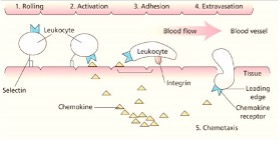
\includegraphics[width=0.4\textwidth]{leuko}
\caption{\label{fig:leuko}}
\end{figure}

\section{TNF alpha}
TNF is the principal mediator of acute inflammation.
Its major source are macrophages and its major effect is the activation of pro-inflammation NFkB transcription factor.
TNF increases the endothelial expression of selectins and integrins, the chemokine production in endothelial cells, macrophage and the production of prostaglandins and leukotrienes (pyrogens, chemotactic).
Furthermore, it induces prostacyclin expression in endothelium, increases local blood flow and increase IL-1 production in macrophages.

\section{Inflammatory response}
The inflammatory response is the body’s natural response that occurs immediately following tissue damage.
 Its main functions are to defend the body against harmful substances, and to promote the renewal of normal tissue.
Signs of inflammation:
\begin{enumerate}
\item pain: due to chemical released by damaged cells
\item swelling or edema: due to an influx of fluid into the damaged region
\item redness: due to vasodilatation (widening of blood vessels and bleeding in joint or structure)
\item heat: due to an increase in blood flow to the area
\item loss of function: due to increased swelling and pain
\end{enumerate}
\noindent
The inflammatory reaction is the combination of a number of overlapping reactions within the body.
Although a lot of these occur simultaneously, a certain order of events may be seen.
The tissue damage may occur from trauma such as a tackle, collision or from a fall.
However, quite commonly tissue injury is as a result of overuse (microtrauma) or pathology
\\
\\
\noindent
When tissue cells become injured, they release a number of chemicals that initiate the inflammatory response.
Examples of these are kinins, prostaglandin and histamine.
These chemicals work collectively to cause increased vasodilation (widening of blood capillaries) and permeability of capillaries.
This leads to increased blood flow to the injured site.
These substances also act as chemical messengers that attract some of the body’s natural defence cells, in a mechanism that is known as \textbf{chemotaxis}.
Although highly beneficial to the body’s defence strategies, some chemicals also increase the sensitivity of the pain fibres in the area and so the area becomes painful.

\section{Leukocytes migration}
Chemotaxis leads to the migration of certain white blood cells to the damaged area.
Two types of leukocytes are predominant in the inflammatory response (macrophages and neutrophils).
Neutrophils are first to reach the injured site and function by neutralising harmful bacteria. Macrophages aid the healing process by engulfing bacteria and dead cells and ingesting them so that the area is clear for new cells to grow.
They arrive at the injured site within the first 72 hours of the injury and may remain in the area for weeks after the injury.

\section{Wound healing in skin}
We have acute inflammation, proliferation, remodelling and then the reprise of the tensile strength.
The synthesis of collagen occurs between 7 and 14 days.
After 14-21 days, we have collagen cross-linking assembling.
Less cross linking means more flexibility and less strength.
There is a control of the immune system to induce tissue regeneration.
\\
\\
\noindent
At the beginning we have pro-inflammatory macrophages phagocyte (type I),  which produce cytokines.
When all the debris has been removed, the macrophages type I become of type II, leading to the downregulation of pro-inflammatory cytokines and tissue regeneration.
Immune tissue engineering is a new approach to drive the transition from type I to type II in order to promote regeneration.
We need to first release few pro-inflammatory molecules (short response) and then tune the transition.

\noindent
The main actors of the immune response following tissue injury:
\begin{itemize}
\item kinetic of immune cell mobilisation after tissue injury
\item initial inflammatory phase following tissue injury
\item immune mechanisms that can impair tissue healing or drive to scarring and fibrosis
\item pro regenerative immune mechanisms
\end{itemize}

\begin{figure}[ht]
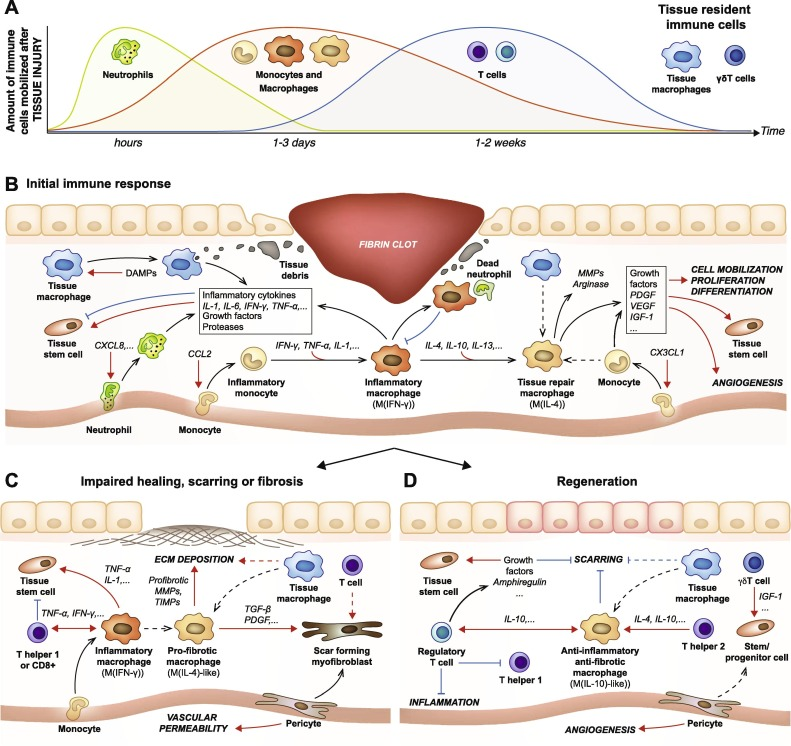
\includegraphics[width=1\textwidth]{healing}
\caption{\label{fig:healing}}
\end{figure}

\section{Strategies to promote tissue regeneration}
Strategies based on biomaterials and drug delivery systems to promote tissue regeneration by controlling the immune system:
\begin{itemize}
\item physicochemical properties of the scaffold. Pay attention to degradability, hydrophobicity, topography…
\item pro-inflammatory modulators
\item anti-inflammatory modulators
\end{itemize}
\noindent
Materials must be chosen according to	protein adsorption, generalised toxic effect, inflammatory cell activation, fibrosis, microvascular changes and tissue-organ specific cell response.

Specific application, tissue-organ type:
\begin{itemize}
\item activation of clotting cascade
\item platelets adhesion activation aggregation
\item complement activation
\item antibody production
\item immune cells response
\item hypersensitivity
\item mutagenesis, genotoxicity
\item tumor formation
\end{itemize}
\noindent
Everything is controlled by the material (type,shape, size, properties) and the environment.
When the biomaterial is recognized as a foreign body, macrophages are recruited and cells will not be able to migrate on the scaffold for regeneration, resulting in a complete failure.

\subsection{Effects of physicochemical modification to biomimetic scaffolds in musculoskeletal applications}
\begin{figure}[ht]
\centering
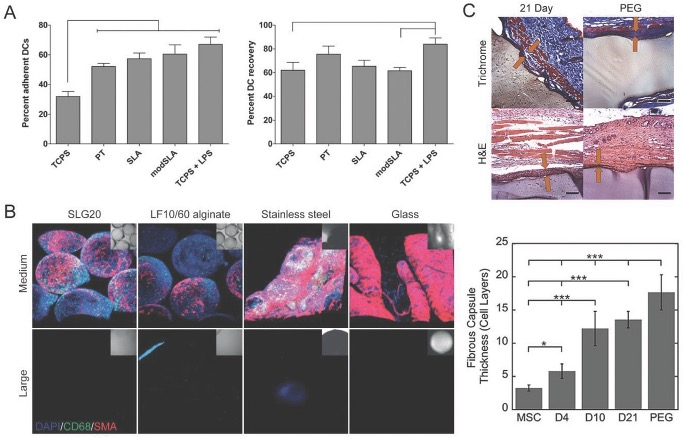
\includegraphics[width=0.5\textwidth]{muscosk}
\caption{\label{fig:muscosk}}
\end{figure}
\noindent
In figure \ref{fig:muscosk} we can check the percentage of dendritic cells(inflammatory cells) in the sample.
We can have a different adhesion degree of inflammatory cells to the scaffold.
Buffering solution + serum (proteins) + antibiotics + growth factors…depending on the absorption we will have a different cell development.
In panel B we see the different shape and thickness for each material.
%chiedere altri appunti su questo, poco chiaro

\subsection{Processes affect the biological outcome}
The aim of this experiment is to evaluate the ability an organic membrane to treat skin burn. Absorption is an important property to take into account, because it causes the inflammatory response.
Keep in mind that proteins can assume different conformations according to specific situation. Three membranes were prepared, they look almost exactly the same.
By increasing crystallinity, the water content is reduced,  leading to different mechanical properties (huge rigidity, increased hydrophobicity = less water absorption for the scaffold).
In vitro tests of the material: fast, easy, not expensive.
In this case they moved materials A and B into further clinical trials. When moving the material in vivo we will have the incubation with human plasma (reproduce bleeding); the aim is to focus on pro-inflammatory signals.
Chemical production: pro-inflammatory cytokines and mixed environment (pro and anti-inflammatory). Moving down there is increase in opsonin.  Some are stretched, as macrophages lead to more adhesion and activation.
We observe low adhesion and high inflammation, this is induced by the material for the scaffold. A small amount of proteins is still able to induce a high pro-inflammatory reaction.

\section{Major activities of macrophages secreted factors}
The main goal of the inflammatory response is healing.
The system will pass through scar tissue formation, modification and finally regeneration. Macrophages react to inflammation through the killing of microbes (nitric oxide)and phagocytosis.
%They should find oxotin, produced by the system.  ???
At the beginning we must defense our body from pathogens and next to build up.

\section{Inflammatory monocytes}
\begin{figure}[ht]
\centering
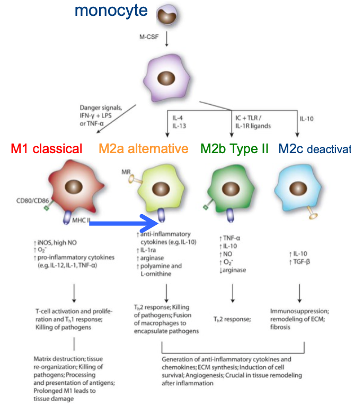
\includegraphics[width=0.4\textwidth]{mono_diff}
\caption{\label{fig:mono}}
\end{figure}

\noindent
In figure \ref{fig:mono} we see macrophages differentiation from classical proinflammatory to regenerative.
Each one is characterized by a specific chemistry.
Maybe we can employ some of these molecules to witness which kind of macrophage is present. After the interaction between material and inflammatory cell, we must find which will be the inflammatory molecules produced afterwards.
Sometimes scaffolds are able to produce new ECM, but not new capillaries.
Our aim is to study when angiogenic factors should be released to induce the regeneration process.

\section{Inflammatory cellular responses}
Opsonin provides the ability for a specific cell to hit the particles and digest them. Phagocytosis involves moving the foreign body from outside to inside within a membrane.
Cancer cells are recognised as foreign since they are coated by opsonin, so they will be eaten by phagocytes.
Cellular responses: oxidative burst, bacterial killing, tissue injury.
If the material is very sensitive, it will release pieces, which are destroyed by macrophages and necrotic surrounding tissue.
The small particles will upregulate the inflammatory response, leading to chronic response.
Our aim is to reduce as much as possible the intensity and time of the defence, the scar tissue.

\begin{figure}[ht]
\centering
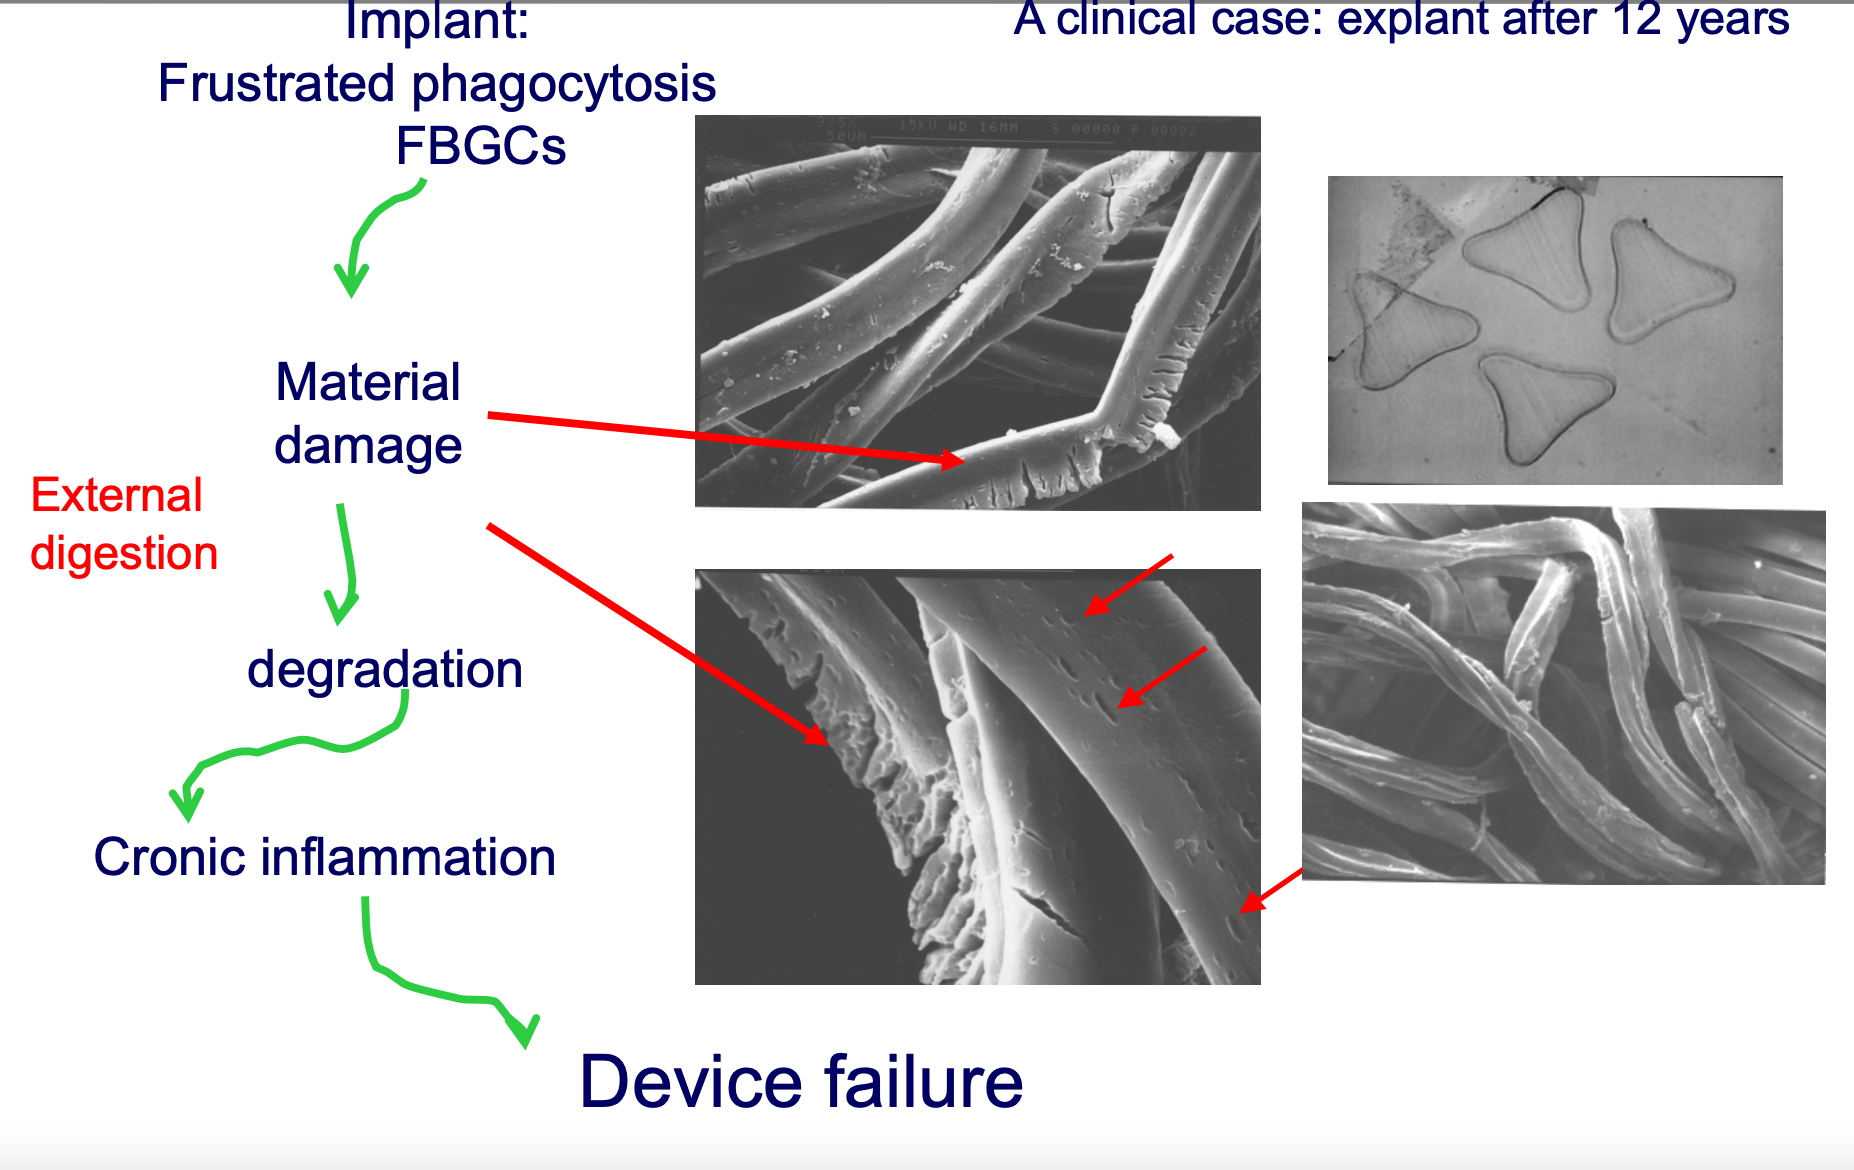
\includegraphics[width=0.6\textwidth]{failure}
\caption{\label{fig:failure}}
\end{figure}
\noindent
Figure \ref{fig:failure}: interaction between cells and material in an implant, explanted after 12 years due to failure.
The tube changed its shape and diameter, provoking blood turbulence, thrombosis risk.
The issue is that spaces were occupied by macrophages, which were able to adhere and digest the external fibers - released in microparticles.
The prosthesis was made in nylon, which is considered to be the most stable polymer e.g. used for parachutes.
Since it is stable and strong, the human body sensed it as foreign and started damaging it. T
he section of the damaged fibers was triangular, while circular fibers had no impact whatsoever.
What does it mean to try to digest a foreign body? The phagocytes digest it piece by piece and this leads to chronic inflammation and failure.

\section{Tissue Healing}
\begin{enumerate}
\item collagenation and cartilarisation
\item angiogenesis
\item proliferation
\item remodelling
\end{enumerate}
\noindent
Once sufficient cleansing of the area has been achieved, the damaged area begins to sprout new capillaries to bring blood to the region - this is known as angiogenesis or revascularization.
When blood flow has been re-introduced to the area, specific tissue cells begin to re-grow.
For example, in a muscle tear muscle cells will repopulate the area.
Wound healing occurs towards the end of the inflammatory process, however the two processes overlap considerably.
\\
\\
\noindent
Macrophages work to clear the damaged area and make space for the regeneration of the new tissue.
After a number of days, fibroblasts (collagen producing cells) begin to construct a new collagen matrix which will act as the framework for new tissue cells.
Tissue healing occurs with the sprout of new capillaries to bring blood to the region (revascularization).
Cellular responses in tissue repair: the capillary should not go randomly, the scaffold architecture should also consider space for angiogenesis.
 We must also ensure a path for interconnection by playing with architecture and release of angiogenetic factors.
\\
\\
\noindent
The proliferation phase lasts 4 weeks.
In cases where the injury has been more severe, the affected area may be composed by a mixture between specific tissue cells (such as muscle cells) and other tissue known as granulation tissue.
If this granulation tissue is not removed it will remain and form scar tissue, which can lead to a decreased functional ability of the tissue.
\\
\\
\noindent
The remodelling occurs when the new cells mould into their surrounding to once again produce a functional tissue.
This process of remodelling can take months even years, altering the new tissue slowly.
The new cells and protein fibers become arranged in a way that is best suited to the stresses imposed on the tissue.
Hence, when a tissue is healing ,it is important to stretch it in the correct direction so to optimise the strength of the new tissue.

\section{Rethinking regeneration: empowerment of stem cell by inflammation}
Immune cells at the site of tissue injury, including macrophages and T cells, secrete TNFalpha, TNFy, IL-1, IL-13 and other pro-inflammatory cytokines, which in turn can activate stem cells.
Once licensed by these cytokines, stem cells can facilitate tissue regeneration though cell differentiation and the release of anti-inflammatory cytokines and growth factors.

\section{Designing immuno informed biomaterials matrices}
We need to provide safety paying attention to tumorigenesis.
There is also the use of extracellular vesicles to load drugs.
We can play with the surface topography or chemistry to design the matrix.
Another aspect that we need to take into account is the macrophage polarization and network formation.
The network should be formed in 3D on the surface, interconnections for macrophages.
For instance, if we have an implanted scaffold we first observe protein adsorption.
After this we have adhesion, macrophages can adhere by forming a network speeding up the process towards regeneration.
Macrophages are also involved in vascularization.
When the scaffold is not porous the macrophages will not be able to polarize and switch to state II, they induce the formation of scar tissue.

\section{Effect of topography and stiffness on macrophages polarisation}
Macrophages assume an elongated shape, M2 like phenotype (up-regulated expression of arginase), on PDMS substrates with 2 gratings topography compared to planar control.
After the adhesion (f), cells start to polarize (g) [figure \ref{fig:topo}] .  Increased stiffness in hydrogel drives the transition in absence of cytokines stimulation.

\begin{figure}[ht]
\centering
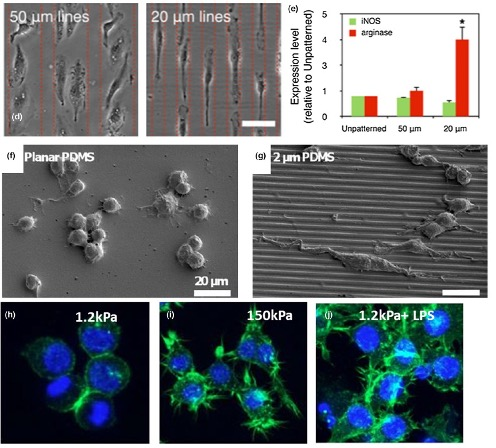
\includegraphics[width=0.5\textwidth]{topo}
\caption{\label{fig:topo}}
\end{figure}

\section{Role of pore size/distribution/degradation}
\begin{figure}[ht]
\centering
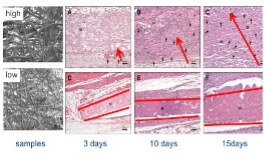
\includegraphics[width=0.4\textwidth]{silk}
\caption{\label{fig:silk}}
\end{figure}

\noindent
Figure \ref{fig:silk}: silk fibroin micro-nets formic acid treated (in vivo evaluations).
In this case we have induced regeneration in unnatural conditions.
Changing the pore size, the mechanical properties will be affected. In high porosity samples: after 3 days we have granulated tissue (dots are cells), the scaffold was able to promote movement inside.
At 10 days the arrows are indicating new capillaries.
Macrophages are at phase II, cells have more space to build tissue.
Then thinner fibers, blood vessels, not so many dots, signalling that inflammatory cells almost disappeared.
Already after 3 days we have a very clear scar tissue formation, which becomes thinner in 10 days.
\noindent
We have also different vascularisation and degradation that depend on porosity.

\section{Possible outcomes after inflammatory response}
After the intervention of macrophages and neutrophils and the death of these latter, our immune system could face three different situations:
\begin{itemize}
\item The situation is clear (no more damage - associated or pathogen - associated signals are detected by the in loco immune cells) and the damage is of moderate extension.
Local immune cells (not only innate but also adaptive immune system cells, after one or two weeks) produce anti - inflammatory cytokines IL-4, IL-10, IL-13, TGF$\beta$, leading to the definition of a pro - resolving environment that leads to macrophages polarization towards the M2 phenotype (this particular phenotype is observable with the microscope: macrophages appear stretched and rich in protrusions).
This phenotype is able to communicate both with local stem cells, allowing for their mobilization, proliferation and differentiation, and with local fibroblasts, triggering scar tissue remodelling: the temporary matrix is digested with appropriate enzymes and a tissue - specific ECM, arranged in a way that is best suited to the stresses imposed on the region, is deposited, leading to healing by regeneration. This process of remodeling can take months or even years.
\item The situation is clear but the damage is too extensive: while the removal of the harmful stimulus leads to the release of anti - inflammatory cytokines and to the polarization of M1 macrophages into M2, and while these are successful into driving the local fibroblasts into a tissue remodelling status, the abundance of the scar tissue itself is a limit to the enzymes’ proficiency: the scar tissue will remain, impacting the mechanical and functional characteristics of the tissue.
\item The situation cannot be cleared. After an appropriate period of time, usu- ally one or two weeks, lymphocytes and plasma cells join M1 macrophages in a context characterized by cyclical instances of tissue healing by repair and tissue damage by immune cells’ oxidizing activity. M1 macrophages are the vast majority, since the situation does not allow for the production of the anti - inflammatory cytokines needed for M2 polarization.
\end{itemize}
\noindent
NB: Since the mechanism of inflammation depends on the blood, non-vascularized tissues are generally hard to regenerate. Different approaches are needed in these cases. An example is a damage to the cartilage - bone interface. The first is a soft, unnerved and non vascularized tissue, while the second one is a robust, innervated and vascularized one. In this situation we need a gradient - rich scaffold that allows for correct tissue and interface regeneration, while avoiding blood vessel formation in cartilage -that would drive the inflammation in the latter and transform it into bone. We can trap vessels in the bone section by playing with porosity, and we could tackle the cartilage section regeneration using injectable biocompatible gels filled with the appropriate cells.

    \graphicspath{{chapters/05/images/}}
\chapter{Biorecognition}

\section{Introduction}

	\subsection{Understanding the ECM}
	Tissue engineering and regenerative medicine require an intimate understanding of the native ECM together with the complexity of cell and tissue biology.
	For therapeutic applications, the basic structure of the ECM should be mimicked using a variety of synthetic or naturally derived materials and fabrication methods.
	The scaffold can be seen as a 3D growth environment which must include:

	\begin{multicols}{2}
		\begin{itemize}
			\item Basic structural properties of the ECM.
			\item Molecular cues to control biological responses.
			\item Protease sensitive site for enabling migration.
			\item Locally delivery of soluble factors for tissue remodelling stimulation.
		\end{itemize}
	\end{multicols}

		\subsubsection{Function of the ECM}
		\begin{itemize}
		\item aids in locomotion
		\item transmits and distributes mechanical loads
		\item prevents premature mechanical failure
		\item partitions cells and tissues into functional units (scaffold architecture)
		\item acts as a scaffold that define tissue and organ architecture
		\item acts as a storage and dissipative devices for elastic energy
		\item acts as substrates for cell adhesion, growth and differentiation
		\end{itemize}
		These functions are defined by composition, structure, mechanical properties and repair response, which depend on tissue type, physiopathology, mechanical forces, damage and healing process.

		\subsubsection{Different states of the ECM}
		\begin{figure}[h]
		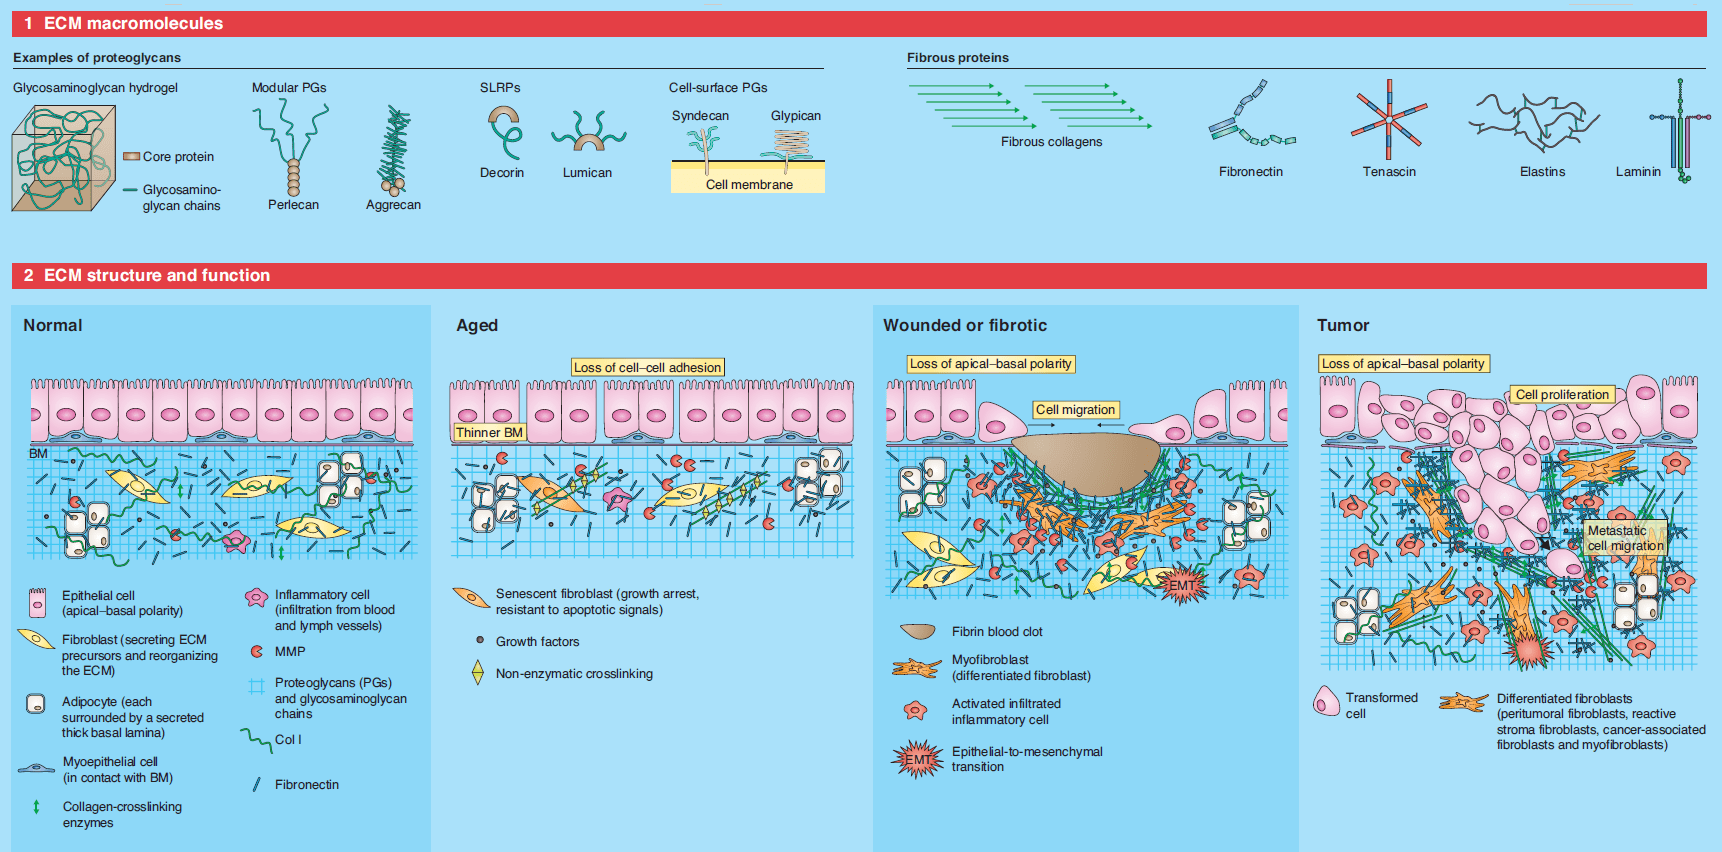
\includegraphics[width=1\textwidth]{ECMfunction.png}
		\caption{\label{fig:ECM} ECM functionalization}
		\end{figure}
		\noindent
		Figure \ref{fig:ECM}:the first example is a normal situation, good substrate. In an aged person we have a loss of elasticity. In the case of a wound, we observe a coagulation cascade and scar tissue formation - which is characterized by a compact tissue. The temporary material (crust) is used as scaffold. We can have healing by repair or regeneration. There is a higher rigidity in the case of temporary material. In the case of a tumour, we have an abnormal growth and migration inside - which they should not be present. The migration is caused by fibers not organising to close the hole.

	\subsection{Surface chemistry: biorecognition in the ECM}
	Cell biology is governed by a complex series of interactions with the ECM.
	It is not enough to promote proliferation, the adhesion involving integrins should also be controlled.
	A pool of molecules is needed, since biological functions are orchestrated by a symphony of signals.
	Communication between cells and the cellular matrix is relevant in the regeneration process.

	\subsection{Biomaterials}
	A biomaterial is a substance that has been engineered to take a form which, alone or as a part of a complex system, is used to direct, by control of interactions with components of living systems, the course of any therapeutic or diagnostic procedure in human or veterinary medicine.
	The aim is to recreate a basic environment before inducing regeneration.
	Proliferation must be upregulated at the beginning to create a population.
	Once the right quantity of cells are in place proliferation needs to be stopped to produce a functional ECM and achieving a therapeutic impact.

	\subsection{Cell - molecules interactions}
	Cells can interact with moving molecules through the gap junctions or through integrins.
	These are sufficient to create communication between neighbouring cells, while travelling molecule are needed for communication between cells far from each other.
	The ECM should not allow for the degradation of these signalling molecules before they reach their target.

		\subsubsection{Maintaining the nutritional status}
		Nutritional status is the bottle neck of tissue engineering, because in big wounds it is difficult to provide nutrition.
		This is due to the fact that blood capillaries are missing from the injured site.
		Because of this angiogenesis must be promoted early in regeneration.
		Hydrogels are an ideal material for promoting angiogenesis because they provide a favourable environment for angiogenesis while providing mechanical support.

		\subsubsection{Cell language}
		The cell language is based on a mapping between micro and nano pattern of the biopolymers that constitute the dynamic nature of the ECM and the receptors on cells that are their complementary binding.
		During cell activity the chemical processes are:

		\begin{multicols}{2}
			\begin{itemize}
				\item Irreversible chemical reactions that provide free energy (ATP $\rightarrow$ ADP) to the cells.
				\item Reversible shape changes in the ECM's biopolymers that provide control over the chemical reactions.
			\end{itemize}
		\end{multicols}

	\subsection{Biocompatible materials: foundation ideas}
	In order to design suitable materials, the biological pathways that lead to normal healing and reconstruction should be known.
	Secondly it is required to develop bio recognition surfaces that turn these pathways on and off.
	To do so it is necessary to know specific affinities for the key molecules found in healing wounds that are associated with vascularised healing and regeneration triggering unnatural local healing.
	If biomolecules are immobilised at the surface, they must be in the correct orientation and conformation.
	Porosity should be engineered to induce vascularisation and decrease the production of fibrotic tissue.
	Furthermore, the modulus matching of scaffold-biomaterial should match with their intended use: modulus mismatch should exacerbate the FBRx.
	Lastly, the engineered scaffold should be able to degrade into non-reactive substances at predetermined degradation rates to serve as a temporary guide for healing.

\section{Cell interactions}
Cells interact with the environment thanks to soluble factors, the extracellular matrix and receptors.
Signals come from the ECM and from neighbouring cells:

\begin{multicols}{2}
	\begin{itemize}
		\item Gene expression regulation leads to adult stem cell differentiation into the lineage of interest.
		\item Tissue specific differentiation.
		\item Survival of primary cells.
		\item interaction with apoptosis: under external stimuli the cells may go to apoptosis.
			This may be useful in case of chemotherapy.
	\end{itemize}
\end{multicols}

	\subsection{Cell adhesion}

		\subsubsection{Molecular mechanism}
		The orientation of ligands is critical for cell adhesion and biological function.
		The RGD sequence promotes cell adhesion and it is usually included in a long peptide so to avoid cell-cell adhesion.
		Depending on the protocol parameters, a nice or absent adhesion can be obtained changing adhesion proteins' orientation.
		This is due to a different density of signal, leading to a different outcome in adhesion.
		When designing a scaffold the aim is to reach an adhesion equilibrium.
		Decreasing the signal density could allow cell movement, promoting migration into the scafffold.
		A stronger signal could promote a fast formation of a cell layer.
		No protein absorption into the scaffold means that there will be no adhesion.
		This can be useful in some cases, for example to avoid thrombus formation in blood vessels or to release cancer treatments from nanoparticles.
		It is clear how cell adhesion depends on the scaffold's surface.
		The conformation and orientation of which can be controlled through cell sensors or screening.

		\begin{figure}[h]
		\centering
		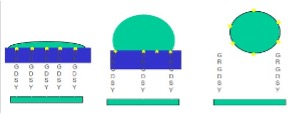
\includegraphics[width=0.5\textwidth]{adhesion}
		\caption{\label{fig:adhesion}}
		\end{figure}

		\subsubsection{Biological process}
		Cell adhesion is a tightly regulated and dynamic biological process.
		It is central to physiological and pathological processes and critical to biomedical and biotechnological applications.
		Adhesive interactions involve:

		\begin{multicols}{2}
			\begin{itemize}
				\item Anchorage that promotes migration and tissue organisation.
				\item Signalling that promotes activation, survival, proliferation and differentiation.
			\end{itemize}
		\end{multicols}

		\subsubsection{Some example of functional tissue assembling}

		\begin{figure}[h]
		\centering
		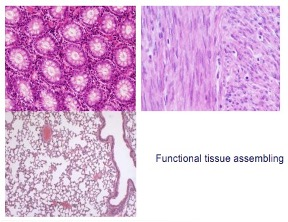
\includegraphics[width=0.5\textwidth]{functionaltissue}
		\caption{\label{fig:funtis}}
		\end{figure}

		In figure \ref{fig:funtis} starting from top left the functional tissue assembling of the radial section of glands , muscles, and lung/alveolar tissue can be seen.
		In the case of muscles, functional tissue should support mechanical stress.
		In glands cells are forming very well polarized capillary tubes for transport.
		For lung tissue blood vessels are present, a small surface and permeability for gas exchange are necessary.
		The air should move into the bloodstream, so the tissue should be very thin and adherent to the vessels.
		There is a low amount of ECM, with the mechanical support is provided by cells themselves.
		It is clear from these examples how the structure is function-dependent.
		Assembly is driven by ECM and adhesion patterning.
		The morphology should depend on the function: for example the thin layer of ECM in the basal lamina formed of collagen fibrils not organized in the classical bundles provides elasticity.

		\subsubsection{Difference between 2D and 3D adhesion}
		Adhesion is completely different in 2D and 3D.
		Cell adhesion is characterized by three stages:

		\begin{multicols}{2}
			\begin{itemize}
				\item Attachment of the cell body.
				\item Flattening and spreading.
				\item Organization of the actin skeleton with the formation of focal adhesion between cell and its substrate.
			\end{itemize}
		\end{multicols}

		The strength of adhesion becomes stronger with the time a cell is allowed to adhere.

	\subsection{Cell - ECM interaction}
	The interaction between cells and matrix can be compared to a chemical reaction where reagents can give rise to a reaction in a specific condition.
	The reactants are the cell and the matrix.
	The reaction takes place only if there is biorecognition: the interaction between cells and the ECM, often mediated by integrins.
	In order to achieve regeneration a number of functionalities must be activated at precise moments.
	The scaffold is a reactant and it is added in the reaction like mechanical stresses.
	The control system should not be downregulated: once the tissue has been regenerated the process must stop.

	\begin{figure}[h]
	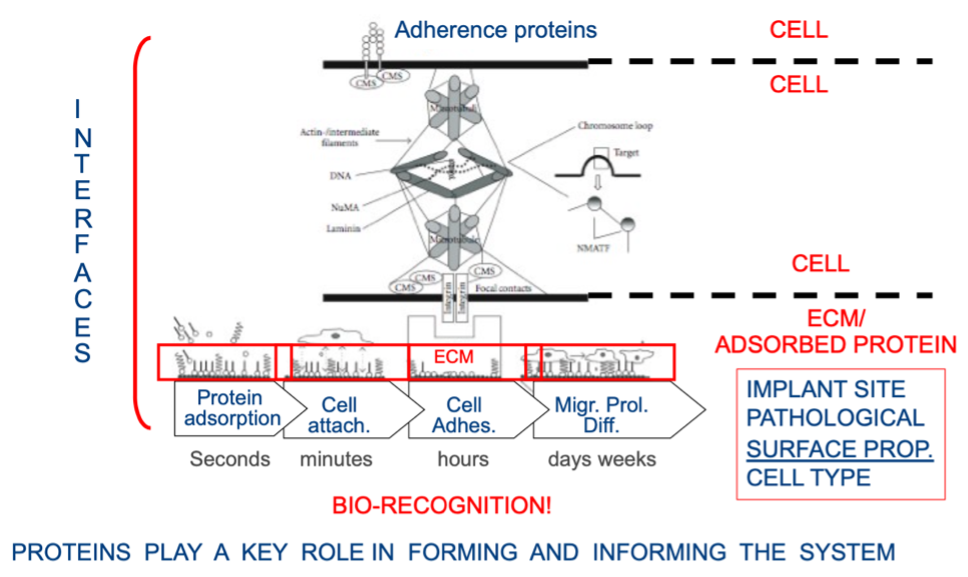
\includegraphics[width=1\textwidth]{interfaces}
	\caption{\label{fig:interfaces}}
	\end{figure}

	\subsection{Cell - scaffold interaction}
	Cells are in suspension in a culture with proteins.
	When the scaffold is inserted in the culture it absorbs a coating of ions, proteins and lipids which are recognized and bound by cells.
	Which proteins will be absorbed depends on the chemical and mechanical properties of the scaffold and the context of implantation.
	The first absorbed proteins will be taken by plasma when bleeding occurs.
	The cells will adhere through integrins if they found ligands in the absorbed proteins.
	Cell adhesion happens only when biorecognition of the scaffold occurs.

		\subsubsection{Scaffold surface}
		Surfaces must be designed in order to control protein absorption.
		Depending on the phenotype of the adherent cells different integrins will be needed.
		The aim when designing a scaffold is to promote cell adhesion through specific integrins so to achieve regeneration.
		Scaffolds and cells are not isolated: the empty spaces between them will be filled by the ECM which will provide proteins and water.
		This adhesion step will determine the failure or the success of the scaffold, making its surface really relevant for its function.
		To achieve the correct surface the scaffold can be functionalized through new chemical groups and its morphology can be changed to drive the interaction between scaffold and cells.

		\subsubsection{Protein absorption}
		The interaction between the implant and biological systems is a dynamic process.
		The biomaterial is characterized by specific properties.
		If the material is incubated in a single protein solution, where the protein is in active conformation, depending on the surface properties, the biomaterial will absorb the proteins, which will remain active, or we will witness deactivation, degradation or modification.

		\begin{multicols}{2}
			\begin{itemize}
				\item Absorption with original conformation: active protein.
				\item Denaturation during absorption: deactivation of the protein.
				\item Absorption with different conformation: different activity, which could lead to unexpected situations.
				\item Degradation: no specific activity, negative response and inflammation, causing the release of small pro-inflammatory peptides are released into the environment.
			\end{itemize}
		\end{multicols}

		The state of the protein is dependent on the scaffold aim.
		This absorption process is dynamic and protein can be released after they are absorbed.

		\subsubsection{Protein substrate}
		The protein substrate is important for the scaffold functionality.
		Changing the material different interactions with proteins can be observed.
		Biocompatibility is a two-way process, the host affects the implant and vice versa.
		Differential adhesion distribution could be observed between domains.

		\subsubsection{Some example of scaffold - cell interaction}

			\paragraph{Polyurethane - an example}

			\begin{figure}[h]
				\centering
				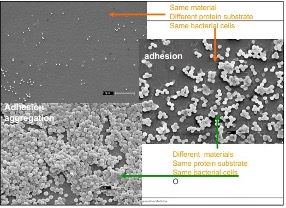
\includegraphics[width=0.5\textwidth]{polyu}
				\caption{\label{fig:polyu}}
			\end{figure}

			In the experiment depicted in figure \ref{fig:polyu} the aim was to produce a surface avoiding bacterial infection.
			The polymer used is polyurethane, used for catheter production where antibacterial properties are really required.
			The surface in contact with different protein substrates leads to different adhesion levels.
			When instead the protein substrate is equal with different materials, adhesion or adhesion aggregation can be seen.

			\paragraph{Vascular graft}

			\begin{figure}[h]
				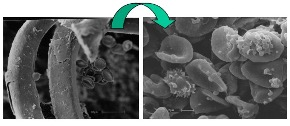
\includegraphics[width=0.5\textwidth]{vascular}
				\centering
				\caption{\label{fig:vascular}}
			\end{figure}

			Figure \ref{fig:vascular} depicts a vascular graft that failed after 6 years of implantation.
			The implant failed because the surface was completely destroyed.
			Bacterial cells  adhered to the implant and activated an inflammatory response.
			Inflammatory cells digested the implant, made of polyester.
			In addition, the implant started to detach in the circulation system  and bacteria were able to attach to red blood cells.
			This is one of the few cases in which we do not want cell adhesion.

		\subsubsection{Cell adherence on the scaffold}
		Cells cannot adhere to synthetic surfaces, as there is no biorecognition and the competition of the ECM is to strong.
		Cell adhesion to synthetic and bio surfaces occurs through a specific receptor interaction with adhesion protein/motifs:

		\begin{multicols}{2}
			\begin{itemize}
				\item Proteins adsorbed from physiological fluids like fibronectin, vitronectin or fibrogen.
				\item ECM components present or deposited by cells like fibronectin, collagen or laminin.
				\item Biospecific sequences engineered on surfaces like RGC or YIGSR for biorecognition.
			\end{itemize}
		\end{multicols}

		Adhesion receptor families are cadherins, selecting, HSPG, integrins and the Ig superfamily.
		Specific integrins act on specific receptors, so there is a need for precision.
		For instance, $\alpha 5\beta 3$ can recognize the ligands into fibronectin, while collagen is recognized by $\alpha 2 \beta 1$.

			\paragraph{Quantifying the adhesion strength}
			To measure adhesion strength centrifugation of a sample is performed and the cells that remain attached to the scaffold are counted.

			\paragraph{Cell adhesion rate}
			Depending on the surface chemistry, there will be different cell adhesion rate.
			According to the protein coating different biological performances will be visible.
			A number of evaluation methods can give us an idea of the adherence strength.

			\paragraph{Scaffold for neuron regeneration - an example}
			Figure \ref{fig:fibrin} depict a designed scaffold for neuron regeneration.
			Adhesion is necessary, but neurons also need to form connections with other neurons.
			The RGD goal is neurite outgrowth, obtained through RGD functionalization.
			The material was provided with fibrin with different level of RGD, the classical adhesion peptide.

			\begin{figure}[h]
				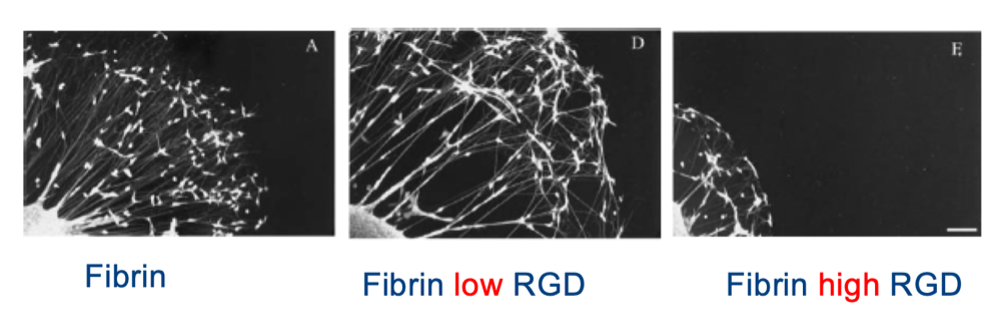
\includegraphics[width=1\textwidth]{fibrin}
				\caption{\label{fig:fibrin}}
			\end{figure}

			A different respone is observed: a good outcome is obtained with a low amount of RGD with a huge number of connections.
			Increasing RGD cause the surface to become more adhesive making the cells to sticky.
			The amount of RGD should resemble the natural one.
			In fibronectin, the RGD content is 1 per chain.
			It is clear here how signal is the combination of the specific ligand and its density.


	\subsection{Cell organization}
	Cells' adhesive interactions with the surrounding ECM defined by the number of adhesive motifs, their distribution and their density and neighbouring cells define cell shape and organisation, controlling functionality.
	This environment regulates the cell survival, differentiation, proliferation and migration.

		\subsubsection{Some examples}

			\paragraph{Chondrocytes}
			Chondrocytes are exposed to compressive forces with an interstitial fluid flow and adhesive cues given by cytokines for cartilage maintenance.
			Chondrocytes are found in a lacuna, where they should behave like pillars and maintain their shape.

			\paragraph{Blood vessel wall}
			Soluble and matrix-bound GFs and flow induced mechanical forces on blood vessel wall, cause cell-cell contacts, and degrade the surrounding basement membrane and stromal ECM in order to migrate and form tubular sprouts.
			Adhesive and mechanical cues drive cell organization.

			\paragraph{Epithelial cells}
			Misregulation of the mechanism induces mechanical and structural changes in the ECM, and transformed epithelial cells migrate towards vasculature and eventually metastasize.

		\subsubsection{ECM controls adhesion and migration}
		ECM-dependent regulators can be associated with 2D, 1D and 3D migration that in turns influence intracellular pathways that govern the migratory phenotype.
		3D migration is defined by pore size and interconnection, the cross linking degree.
		Aligned fibers are randomly distributed with low density in the scaffold.
		Adhesion and migration are controlled by the ECM composition, stiffness of the material and ligand density.
		An aligned topography of fibres allow to obtain different architectures.
		In the case of a mixed fibrous scaffold, aligned and random, fibres are present with an elastic behaviour, exacerbated by cross linking.
		Sending seed cells on the different structure, diverse behaviour for orientation, migration, proliferation, growth and differentiation will be obtained.
		Architecture can play a huge role in scaffold functionality.

			\paragraph{Contractility}
			The substrate contractility regulates 3D migration, regardless of pore size.
			When a cell lands on a stiff fiber it can adhere, but it becomes very stable and not able to modify its shape or migrate.
			Instead cells on soft fibers are able to move and form protrusions.
			Since cells in nature are connected to ECM fibers, when they move the ECM will also follow the contraction of the cell body.
			If the cell adheres to soft fibers, the same natural movement can occur.
			When the substrate is too rigid contraction cannot occur and healing will be different.
			The scaffold should be soft enough to follow the reorganization needed by the cells.

			\paragraph{Mineralization}

			\begin{figure}[h]
				\centering
				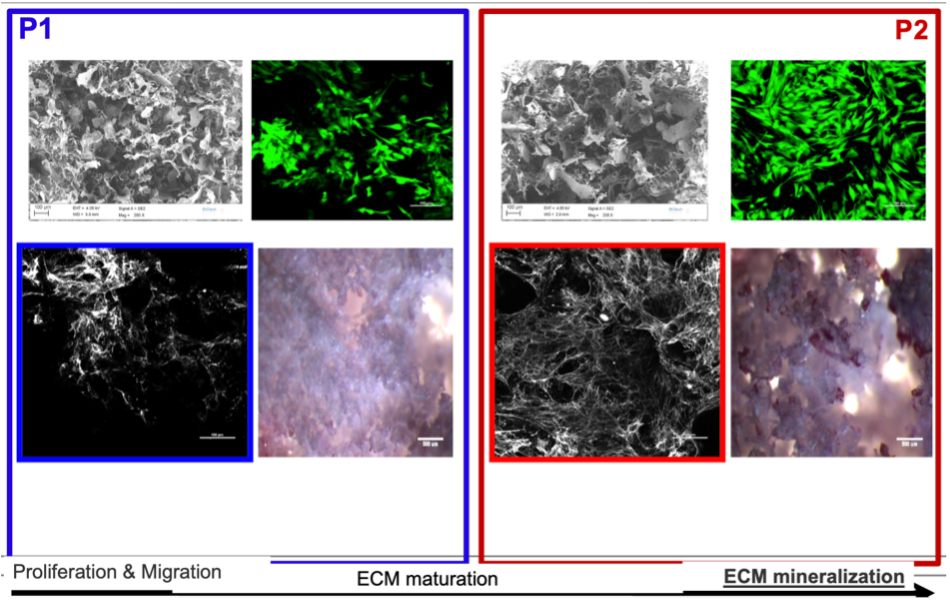
\includegraphics[width=0.7\textwidth]{mineralization}
				\caption{\label{fig:min}}
			\end{figure}

			Figure \ref{fig:min} depicts two scaffolds prepared with the same polymer different for pore size and distribution.
			The scaffolds are built for bone regeneration: the presence of collagen fiber in a continuous network should be considered.
			Osteoblasts should infiltrate the scaffold for building the network and the porosity should allow this.
			Once the network is formed, hydroxy apatite is deposited on top of the collagen fibers.
			While in P2 the cell distribution is uniform, in P1 it is clustered because interconnection is not complete.
			These clusters don't allow a continuous network to be built due to tight collagen and the lack of mineralization.
			In fact when cells are not able to migrate, mineralization cannot occur.

			\paragraph{Capillary formation}
			A continuous network is required for capillary formation.
			The parameters can be fully controlled with scaffold design.
			In order to improve the performance of the P2 scaffold we could functionalize it with collagen or drug release systems.

		\subsubsection{Reproducing in vitro a working environment}
		The scaffold surface interacts with the cell through the ECM during biorecognition.
		The aim is to reproduce in vitro a working environment, working for the cell and solving a specific task.
		Depending on the context, the bioreaction can happen: the cell recognizes the surface of the scaffold if it is functionalized or for protein absorption.
		Cell population, and integrins, are context specific.

	\subsection{Methods for modulating receptor-ligand interactions}
	To modulate receptor-ligand interactions, one could control:

	\begin{multicols}{2}
		\begin{itemize}
			\item Natural ECM biomaterials: biologically relevant environment, but poor mechanical properties and inconsistent reproducibility.
			\item Whole ECM adsorption.
			\item Synthetic linear binding motif: surface functionalization.
				There is a need to define the density of the signal, the protein of interest, the stability (quantify the time for which the signal should remain), orientation, homogeneous or pattern distribution.
			\item Spatially oriented binding motif.
			\item Nanopatterning with nanolithography: mix different molecules and patterns, as well as technologies.
			\item ECM-like biomaterials.
		\end{itemize}
	\end{multicols}

\section{Biorecognition requirements}
The biorecognition process will have a good outcome only if the absorbed proteins are the right ones according to the following parameters:

	\subsection{Absorbed protein recognition}
	The absorbed proteins must contain sequences (ligands) recognizable by dedicated cellular receptors: among the first we remember RGD, YIGSR, IKVAV and RETTAWA, among the second we cite integrins.
	Integrins are heteromeric transmembrane receptors that mediate cell - ECM interaction with different glycoproteins among whom fibronectin and vitronectin and collagen fibers.

	\subsection{Ligand orientation}
	The ligands mentioned above must be oriented outward, they must not be hidden or used by the scaffold to link with the proteins.
	If this happens, the sequences won’t be able to be recognized by the cellular receptors.

	\subsection{Stability}
	The absorbed proteins must have a stable structure: they must not denature, take on conformations with unexpected functions like prions or hold native functions that could hinder the regenerative process like trigger clotting formation or release peptides that could be pro-inflammatory, leading to chronic inflammation.

	\subsection{Concentration}
	The array of absorbed protein must expose the right number of ligands, with the right density.
	In particular for the regenerative aim, the ligands need to be in the right number and density to allow for macrophage adhesion while still allowing them to move.
	They need also to stretch across the binding sites, since this stretching has been correlated with the polarization towards the M2 phenotype for macrophages.

    \graphicspath{{chapters/06/images/}}
\chapter{Hydrogels}


\section{Introduction}
Hydrogels were the first biomaterials rationally designed for human use, especially for soft tissue engineering.

	\subsection{Composition}
	They are a particular class of materials, exhibiting both solid-like and liquid-like properties, consisting of hydrophilic polymer chains and water that occupies the interstitial spaces or pores that are defined in the 3D network constituted by the cross-linked polymeric chains.

	\subsection{Water content}
	Water is the major constituent of hydrogels and could reach more than $90\%$ of the weight of the material.
	Its quantity is dependent on the degree of hydrophilicity of the polymer chains.

	\subsection{Seeding with cells}
	Cells can be added inside the hydrogel before or after gelatization.
	In the first case, one must make sure that the gelatization itself won’t damage the cells.
	In the second case, porosity must allow for uniform cellular colonization.

\section{Characteristics}
Hydrogels’ characteristics can be modulated according to three main variables:

\begin{multicols}{3}
	\begin{itemize}
		\item Chain composition.
		\item Cross-linking nature.
		\item Network nature.
	\end{itemize}
\end{multicols}


	\subsection{Chain composition}
	Hydrogels can be natural (usually polysaccharides) or synthetic polymers.
	The main subvariables are:

	\begin{multicols}{2}
		\begin{itemize}
			\item Chain length.
			\item Degree of hydrophilicity.
			\item Presence of ligands recognizable by cellular receptors.
				The utility of synthetic polymers is that they can be functionalized with these kinds of ligands to allow cell adhesion, but degradability will become a problem.
		\end{itemize}
	\end{multicols}

	\subsection{Cross-linking nature}
	With cross linking or gelatization nature is intended the strategy employed to connect the polymeric chains

		\subsubsection{Chemical cross-linking}
		The polymer chains are covalently linked.
		This linkage can be obtained in an enzymatic way if enzymes capable of interacting with the chosen polymers exist.
		The enzymatic cross-linking is useful because it guarantees the degradability of the scaffold via host enzymes or in a non-enzymatic way, exploiting specific reactions that may require specific reagents.

		\subsubsection{Physical cross-linking}
		In physical cross-linking, polymer chains are held together by molecular entanglements (a temporary spatial constraint) and secondary forces such as ionic, hydrophobic, and hydrogen bonds.
		Chemically crosslinked hydrogels always present some degree of physical interaction as well, but the contrary, of course, does not occur.
		Physical crosslinking can be obtained via thermal treatment, pH changes and treatment with organic solvents.

	\subsection{Network nature}
	Network nature: it’s the overall 3D structure defined by the crosslinked polymers.
	Its main characteristic are the number and the dimension of the interstitial spaces or pores, influenced by polymer chains length and by the number of crosslinkings.
	Pores number and dimension, together with the degree of hydrophilicity of the polymer chains, will determine the maximum amount of water hosted by the hydrogel.
	This in turn will impact the swelling capacity, one of the main characteristics of these kinds of scaffolds.

\section{Other uses of hydrogels}

	\subsection{Hydrogels as cells carriers}
	Hydrogels can also be designed with the only goal of carrying modded cells to a particular region of the body: in that case non biocompatible, non biorecognizable synthetic polymers can be used to avoid premature hydrogel degradation and unwanted interaction with the cargo and to carry the cells to the targeted location.

	\subsection{Hydrogels as drug releasing systems}
	Hydrogels can be used as drug release system: they can function as surrogate matrices to carry modified cells producing a specific therapeutic agent.
	In order to protect these cells from the host’s immune system, the hydrogel itself must be coated by a semipermeable membrane, that must allow the entrance of nutrients and growth factors in the hydrogel and the exiting of the therapeutic products.
	
\section{Injectable hydrogels}
The tunable physical properties, excellent biocompatibility, facile preparation, and ease of administration with minimal invasiveness of injectable hydrogels (IHs) has made them excellent candidates to solve the clinical and pharmacological limitations of present systems for multitherapy. 
Notably, their porous structures, formed due to the three-dimensional network of hydrogels, permit therapeutic agents to be well adhered and entrapped in hydrogels. Also, the kinetics of therapeutic agent release from hydrogels can be controlled by regulating their porous structure in addition to components.

    \graphicspath{{chapters/07/images/}}
\chapter{Fetal healing}

\section{Scarring}
A scar is a densely packed disorganized collagen bundle, with absence of hair follicles, sebaceous glands and other appendages.
Scarring and fibrosis dominate some diseases in every branch of medicine and surgery.
Examples: skin incisions heal with scars (pathological processes as keloids, hypertrophic scars, …).

\subsection{Adult scarring}
The mechanism of scar formation involves inflammation, fibroplasia, formation of granulation tissue, and scar maturation.  The acute inflammatory response (pro inflammatory mediators) is followed by the proliferation of fibroblasts, which are cells responsible for synthesizing various tissue components, including collagen and fibrin. During the acute inflammatory phase, circulating progenitor cells migrate to injured tissue. Rapid cellular proliferation occurs, which ultimately results in the formation of new blood vessels and epithelium. Fibroblasts then differentiate into myofibroblasts, which are the cells responsible for collagen deposition and wound contraction. Scar formation ultimately results from excess accumulation of an unorganized extracellular matrix. Although scar remodeling occurs for months to years after the initial injury, complete restoration of the normal extracellular matrix architecture is never achieved.

\section{Embryonic healing}
In contrast to adult wounds, early gestation fetal skin wounds repair rapidly and in the absence of scar formation.
The fetus is able to regenerate tissues by assembling collagen fiber in a well organised structure.
The biology of fetal repair must be understood; in particular, cellular and matrix events may provide insights to help to modulate adult wound repair to become more fetal-like.

\subsection{Fetal extracellular matrix}

We should try to mimic the embryonic development procedure, where the ECM is elaborated in parallel with cell differentiation and growth.
In particular, our aim is not to obtain a normal ECM analogue (mature scaffold), but a wound bed matrix analogue suitable for regeneration.
Collagen represents a "mature" scaffold, forming a microenvironment suitable for fully differentiated cells.  If we build a scaffold based on collagen type I, cells which don't usually reside in an ECM made extensively of collagen type I will not interact with the surface, leading to a pathologic response. Example: chondrocytes usually interact with collagen type II, so if collagen type I is present cells will form fibrocartilage.
\\
\\
\noindent
The fetal extracellular matrix is optimized to facilitate cellular migration and proliferation, which may have important implications in wound healing.
\begin{itemize}
\item collagen content: high content of collagen type II and V, increased collagen synthesis.
\item hyaluronic acid: in scarless fetal wounds, the hyaluronic acid content of the extracellular matrix is increased more rapidly than in adult wounds, major component.
\item adhesion proteins: scarless fetal wounds have an enhanced ability to up-regulate extracellular matrix adhesion proteins, such as tenascin and fibronectin
\item ECM modulators: fibromodulin inactivates transforming growth factor (TGF)-beta, a key cytokine involved in wound healing, and has been shown to have an antiscarring effect during wound repair.
\item non-sulfonated GAGs
\end{itemize}

\subsection{Fetal mediators of scarless repair}
\begin{itemize}
\item lack of inflammation: decreased platelet degranulation and aggregation,  anti-inflammatory cytokines
\item fibrobrlast cells with high migration rate (affecting collagen depth and cross linking)
\item increased number of HA receptors
\item myofriboblasts appear earlier and then disappear
\end{itemize}

\begin{figure}[h]
\centering
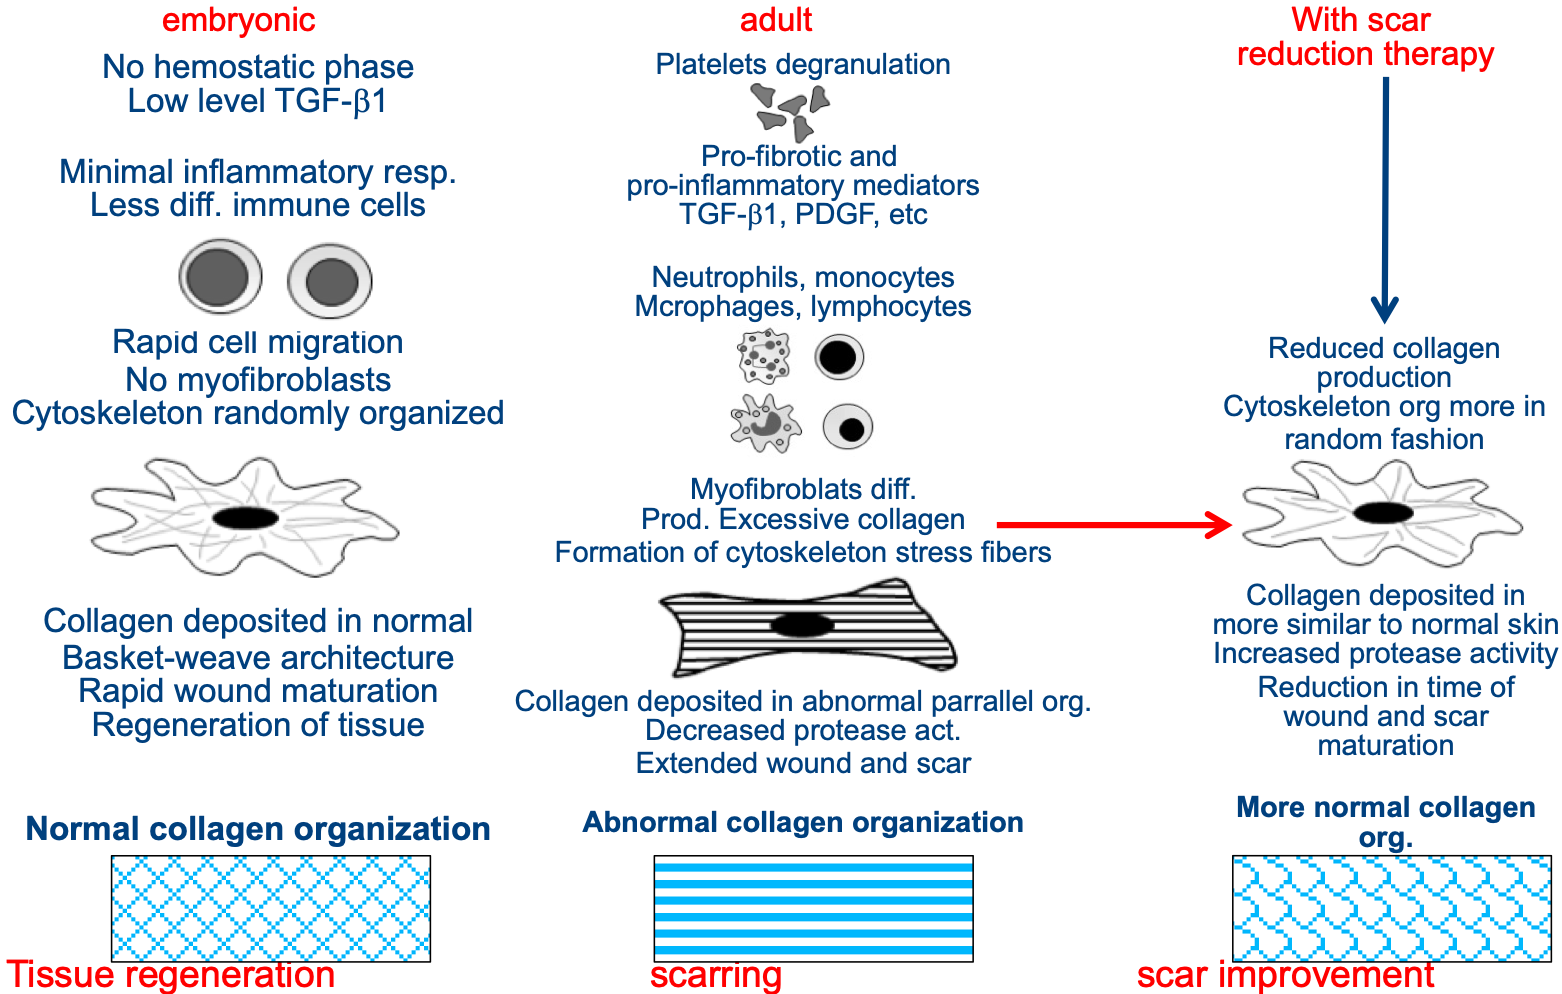
\includegraphics[width=0.5\textwidth]{scar.png}
\caption{\label{fig:scar}A lesson from fetal healing: scarless regeneration}
\end{figure}

\section{Hyaluronan}
Hyaluronan is a hydrated gelatinous material	synthesized from basal side of an epithelial sheet.
It creates a cell-free space into which cells can proliferate and migrate, perform the diffusion of nutrients, metabolites,...
It is able to resist compressive forces and acts as space filling material in embryogenesis.
It is degraded by hyaluronidase.
\\
\\
\noindent
Hyaluronian is composed by the simplest GAG with a very long chain length (25000 disaccharide units. It lacks sulfated sugars and is usually not attached to protein (used as filler). The high negative charges on the glucuronic acid attract Na+ ions and water.

%\section{Collagen assembly}
%Collagen type III is involved in structural maintenance in expansible organs e.g. smooth muscle, blood vessels, connective tissue. Collagen type V instead is responsible for fibril formation in skin, bones and fibrocartilage. In particular,  collagen fibrils have a high content of collagen type III and IV.

\section{Biology of regeneration}
Regeneration of amputated limb can occur at an adult stage in amphibians and fish.
This complex process is enabled by specific tissue regeneration mechanisms.
For instance,  in adults of Homo Sapiens the liver regenerates spontaneously.
Furthermore, we have little capacity to regenerate tendons and ligaments.

    \graphicspath{{chapters/08/images/}}
\chapter{Scaffold design}

\section{Introduction}
Tissue engineering is the 3D assembly over time of vital tissues-organs by a process involving cells, signals, and the extracellular matrix.
The dynamics of regeneration vary from tissue to tissue according to the hierarchy of tissue or organ function.

    \subsection{Material design}
    A biocompatible material must have the ability to perform a specific application with an appropriate host response.
    The main consideration to be made when designing a material are:

    \begin{multicols}{2}
        \begin{itemize}
            \item sourcing of functional cells: if the scaffold requires a pre-loading of cells, the type of cell needed and where to obtain them need to be decided.
            \item GF regulatory systems: synthetic polymers with no biorecognition properties require functionalization>
            \item immuno acceptance:  for example force stem cells to become osteoblasts or modulate the immune response in order to shorten the inflammation and boost regeneration.
        \end{itemize}
    \end{multicols}

    Biological information is required for performing in vitro tests and for functionalization that needs to be linked to specific biological pathways and is essential to thoroughly describe the mechanisms.

    \subsection{Scaffold categories}
    Scaffolds can be grouped in two categories:

    \begin{multicols}{2}
        \begin{itemize}
            \item Conductive.
            \item Inductive.
        \end{itemize}
    \end{multicols}

        \subsubsection{Conductive scaffolds}
        Conductive scaffolds provide and maintain a 3D environment that supports a passive cell infiltration, creating a pseudo micro environment.
        Their limitation is that they are not able to provide enough information to promote full regeneration in most applications.

        \subsubsection{Inductive scaffolds}
        Inductive scaffolds are designed to closely mimic the native cellular environment and may contain bioactive molecules and naturally or synthetic analogues of structural, functional or specialised proteins and proteoglycans.
        They can increase the biocomplexity of the system.

    \subsection{Scaffold function, composition and geometry}
    A scaffold is part of a complex system.
    It is used to direct, by control of interactions with components of living systems, the course of any therapeutic or diagnostic procedure.
    A scaffold is composed by different materials like natural and synthetic polymers.
    The geometry should be suitable for the specific application: it should allow migration, distribute cell in a functional manned and align them.
    Polymers can be combined with other materials or drugs.
    If the interaction and biocompatibility are present, there will be a suitable response.

    \subsection{Tissue engineering strategies}
    There are different tissue engineering strategies:

    \begin{multicols}{2}
        \begin{itemize}
            \item Just scaffold in vivo: the body helps with the regeneration, if possible it’s the best strategy that can be followed.
            \item Scaffold and cells implantation: need to define why we wish to culture and what to culture in vivo.
                Possible explanations are ECM production and differentiation.
            \item Cell sheet engineering: fabrication with stem cells from the patient.
                It is the only bottom-up approach, starting from the material and not from the biology.
        \end{itemize}
    \end{multicols}


    \subsection{Biocompatibility requirements}
    Revised performance criteria for the 4th generation of biomaterials are:

    \begin{multicols}{2}
        \begin{itemize}
            \item Tailored biodegradation.
            \item Amenability to engineering design and manufacturing.
            \item Induces cell and tissue integration.
            \item Smart: physiologically responsive.
            \item Instructional: controls cell fate.
            \item Mechanical strength and function: mechanical signalling.
        \end{itemize}
    \end{multicols}

        \subsubsection{Sponge for trabecular bone regeneration}
        \begin{figure}[h]
            \centering
            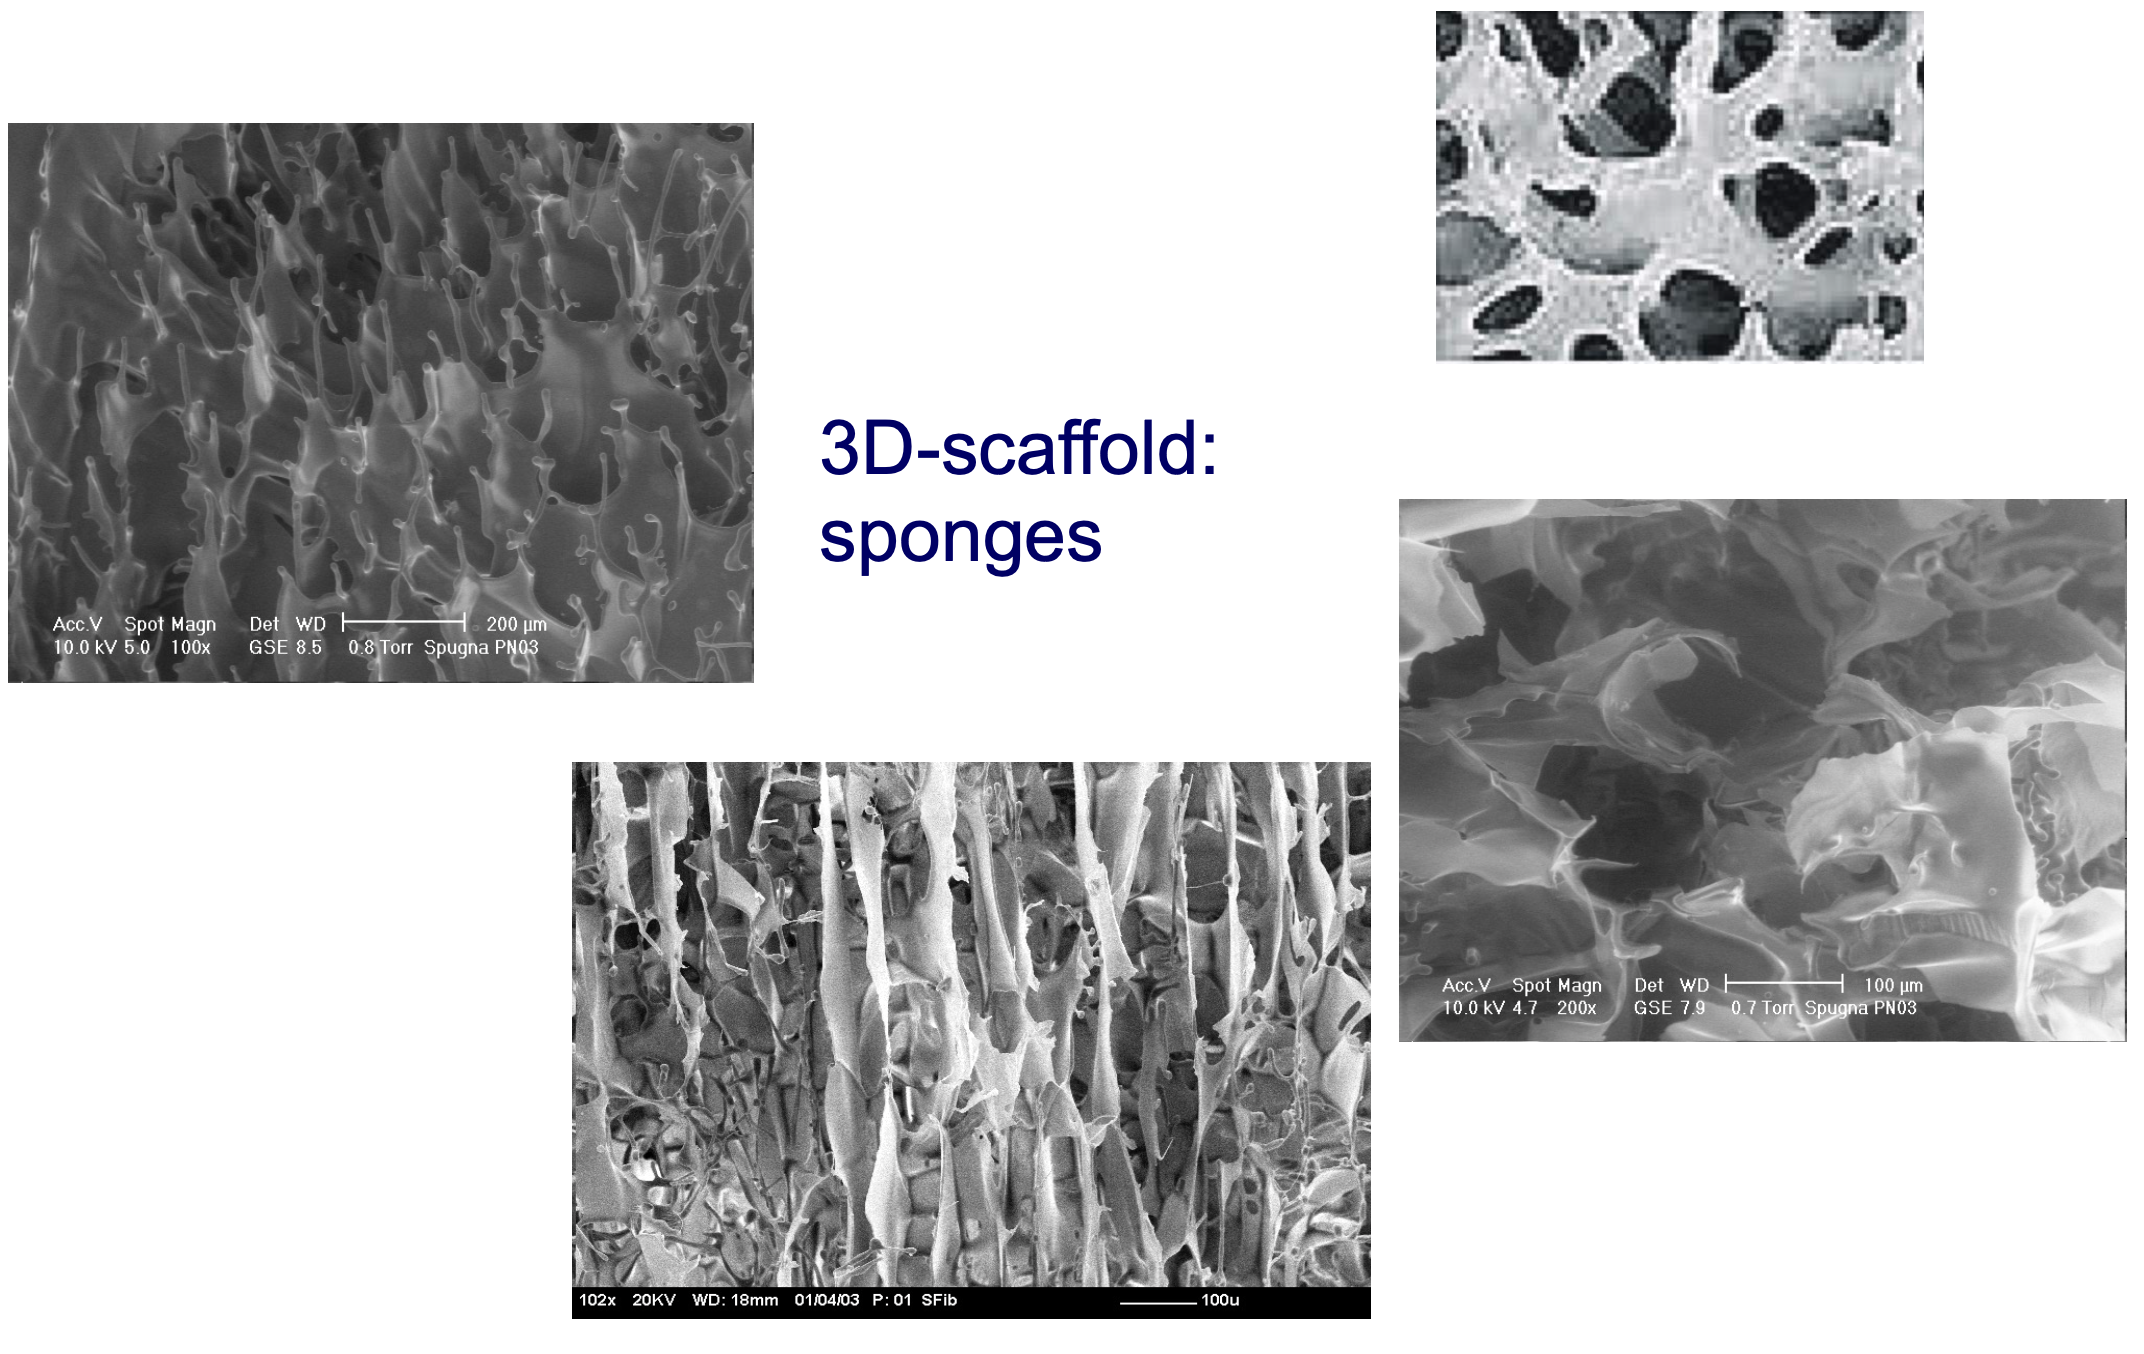
\includegraphics[width=0.5\textwidth]{sponge.png}
            \caption{\label{fig:sponge}}
            \end{figure}
        \noindent
        Fig \ref{fig:sponge} depicts the repair of trabecular bone with 3D-scaffold sponges.
        All of the images represent artificial scaffolds except the one on the top right depicts the natural sponge.
        The porosity can be oriented or random, with different geometries.
        The scaffold should promote adhesion, proliferation and migration.
        Hypoxia should be avoided, maybe with early angiogenesis.
        In vivo: in the case of bones, we have osteoblasts adhesion and migration, ECM production.
        In order to avoid hypoxia and necrotic tissue formation it is required to achieve vascularization, oxygen must be supplied to stimulate angiogenesis.
        In vitro: to test the scaffold in vivo it could be cultured in a bioreactor, a chamber with perfusion and a dynamic environment.


    \subsection{Scaffold examples}

        \subsubsection{Muscle regeneration}

        \begin{figure}[h]
            \centering
            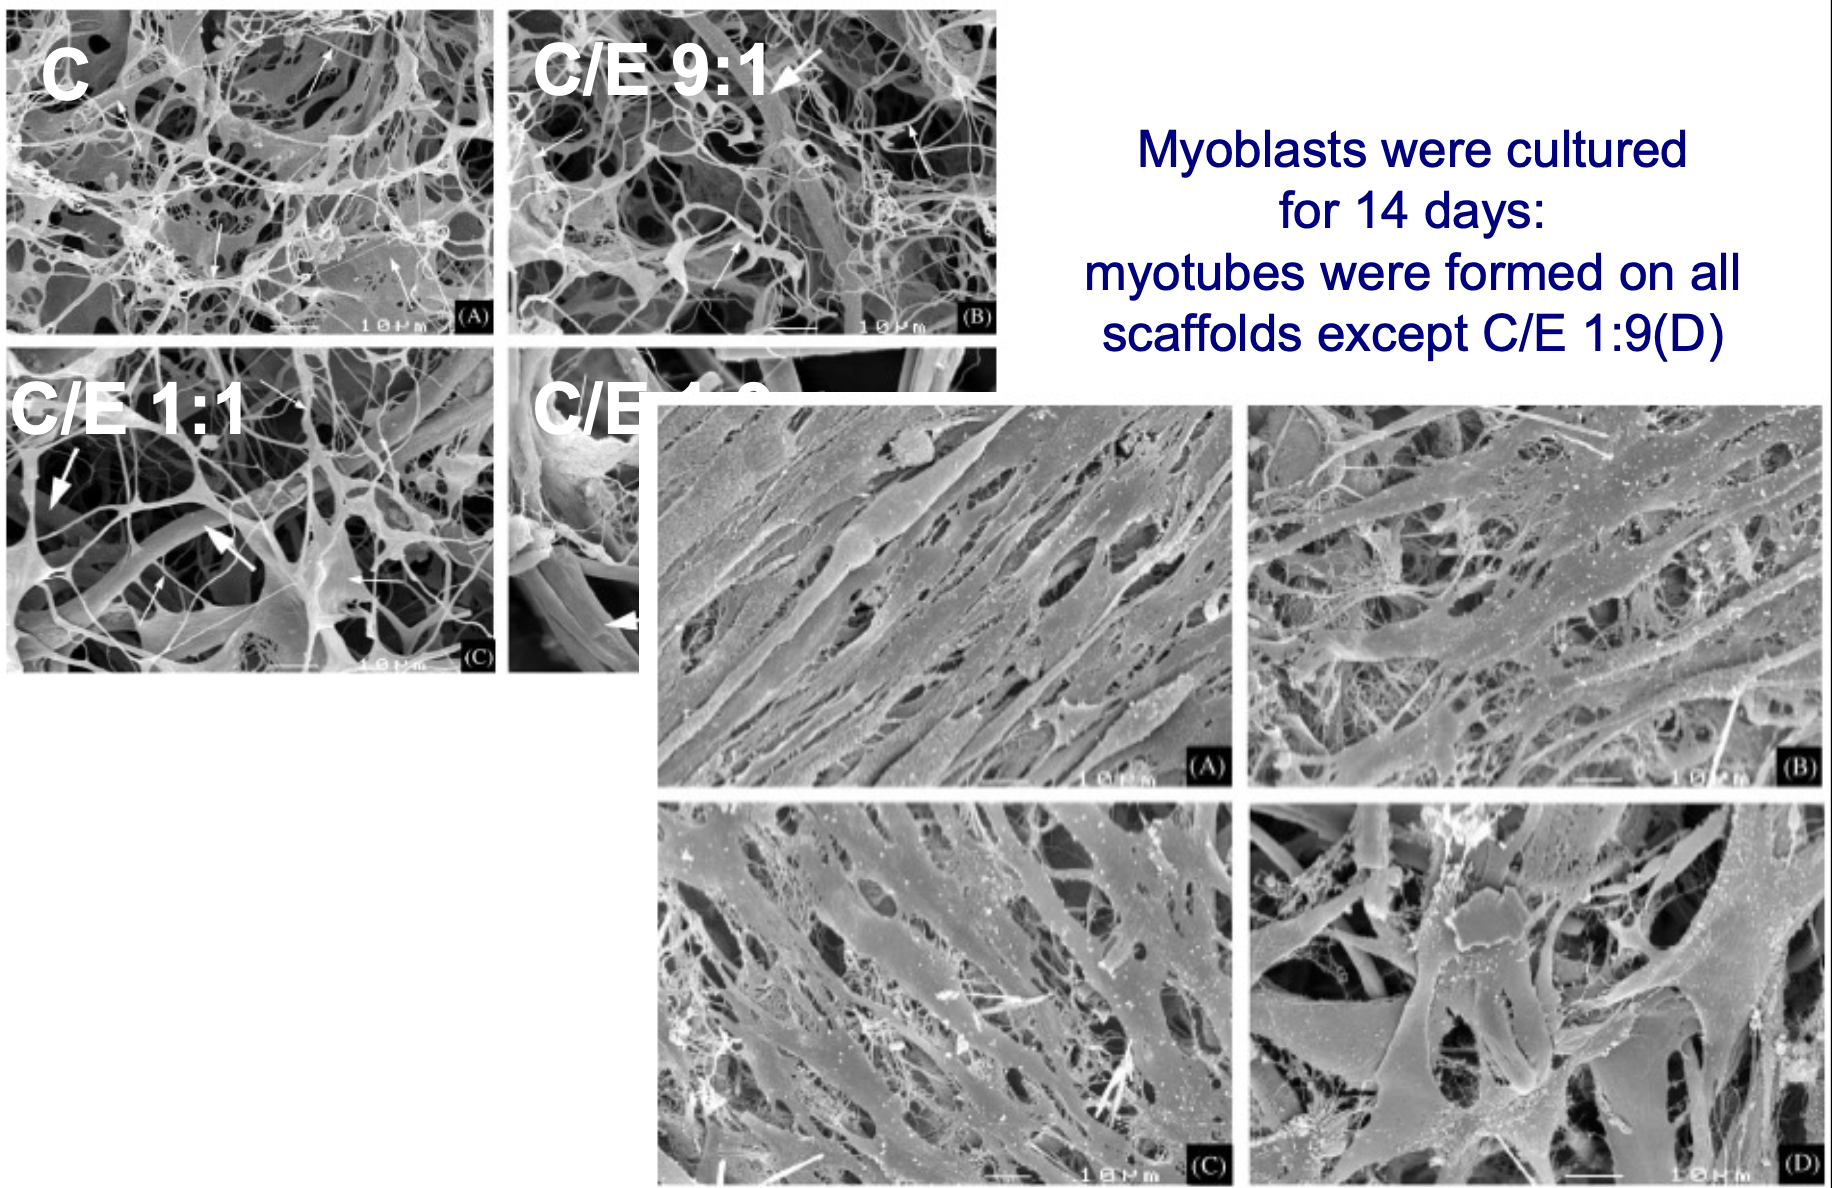
\includegraphics[width=0.5\textwidth]{myoblast.jpg}
            \caption{\label{fig:myoblast}}
        \end{figure}

        Fig \ref{fig:myoblast} depicts muscle regeneration.
        Collagen, elastin and glycosaminoglycans have been used.
        GAGs control water content and mechanical properties.
        Elastin is required for muscle elasticity and collagen for the strength.
        It is necessary to find the optimal ratio among the components.
        By changing the ratio  four different architectures are observable:

        \begin{multicols}{2}
            \begin{enumerate}
                \item C: sponge, similar to natural behaviour of collagen.
                \item C/E 9:1: big fibers starts to appear thanks to elastin.
                \item C/E 1:1: similar content to C/E 9:1.
                \item C/E 1:9: a lot of big fibers are present.
                    Pink fiber are elastin fibers.
            \end{enumerate}
        \end{multicols}

        C might not be optimal, as well as C/E 1:9, as they are quite different from biological setting.
        In vitro test: after two weeks myoblasts were cultured for 14 days and myotubes were formed on all scaffolds except C/E 1:9(D).
        A different organisation of the myotubes is observed.
        In the last example, myoblasts are not able to organise as the condition is to far from physiology.
        By considering the test, the best samples seem to be C/E 9:1 and C/E 1:1 .

        \subsubsection{Bone regeneration}

        \begin{figure}[h]
            \centering
            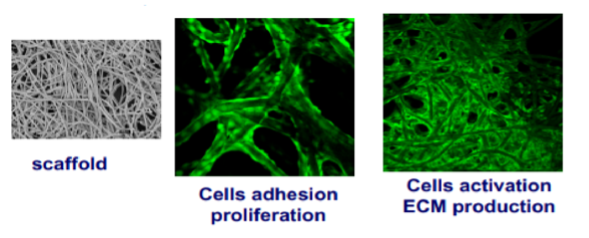
\includegraphics[width=0.6\textwidth]{3D.png}
            \caption{\label{fig:3D}}
        \end{figure}

        Figure \ref{fig:3D} represent a scaffold for bone generation and osteoblast proliferation.
        The cells, in green, are able to adhere, proliferate and migrate.
        The scaffold is then completely covered in cells.
        We then witness tissue-specific ECM production and mineralzation.
        This is a great starting point, but the degradation process of the scaffold and vascularization still need to be understood.
        In vivo vascularization can be checked performing co-culture of osteoblasts giving the angiogenesis factors and the collagenic structure for capillary network formation and endothelial cells that use empty spaces to assemble as a tube.
        It is clear that to obtain a physiological situation careful design is needed.

        \subsubsection{Polymer seeded with different cells}

        \begin{figure}[h]
            \centering
            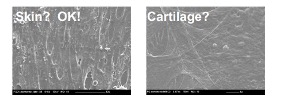
\includegraphics[width=0.6\textwidth]{sk_car.jpg}
            \caption{\label{fig:sk_car}}
        \end{figure}

        Fig \ref{fig:sk_car} depicts two film composed of the same polymers with the same architecture but seeded one with keratinocytes and the other with chondrocytes.
        The two films were completely spread.
        Cells grown in a flat dish tend to behave as individual cells or forming a monolayer, whereas cells cultured in a 3D space are more likely to assume the characteristics of a particular tissue.
        Cartilage, once grown flat, is almost impossible to shape into joints.
        The scaffold here, in the case of cartilage, is inducing the loss of the original phenotype, so it is not biocompatible.
        In the case of the skin, it is promising for biocompatibility, forming compact and well connected monolayers.

        \subsubsection{Scaffold for bone regeneration}

        \begin{figure}[h]
            \centering
            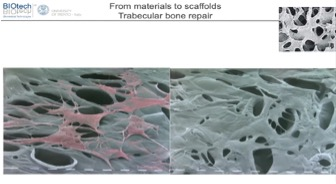
\includegraphics[width=0.5\textwidth]{bone.jpg}
            \caption{\label{fig:bone}}
        \end{figure}

        Fig \ref{fig:bone} depicts a polymer used for bone regeneration.
        In this case there is biocompatibility at all: the cells adhere to the polymer but do not migrate.
        To tackle this problem porosity should be increased.
        After few days a multi-layer structure is obtained, without migration and biocompatibility.

        \subsubsection{Seeding with suing urothelial cells}

        \begin{figure}[h]
            \centering
            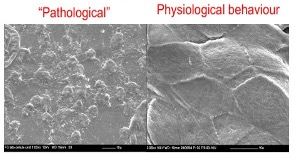
\includegraphics[width=0.5\textwidth]{suine.jpg}
            \caption{\label{fig:suine}}
        \end{figure}

        Fig \ref{fig:suine} shows suine primary urothelial cells, 6 days after seeding.
        The right image has the geometrical shape of the cells so the phenotype is ok.
        In the right image cells don’t connect and are disorganised, so they do not communicate.
        They have a more round shape, so the adherence is not good and there is no activation.

        \subsubsection{Fibroin micronet}

        \begin{figure}[h]
            \centering
            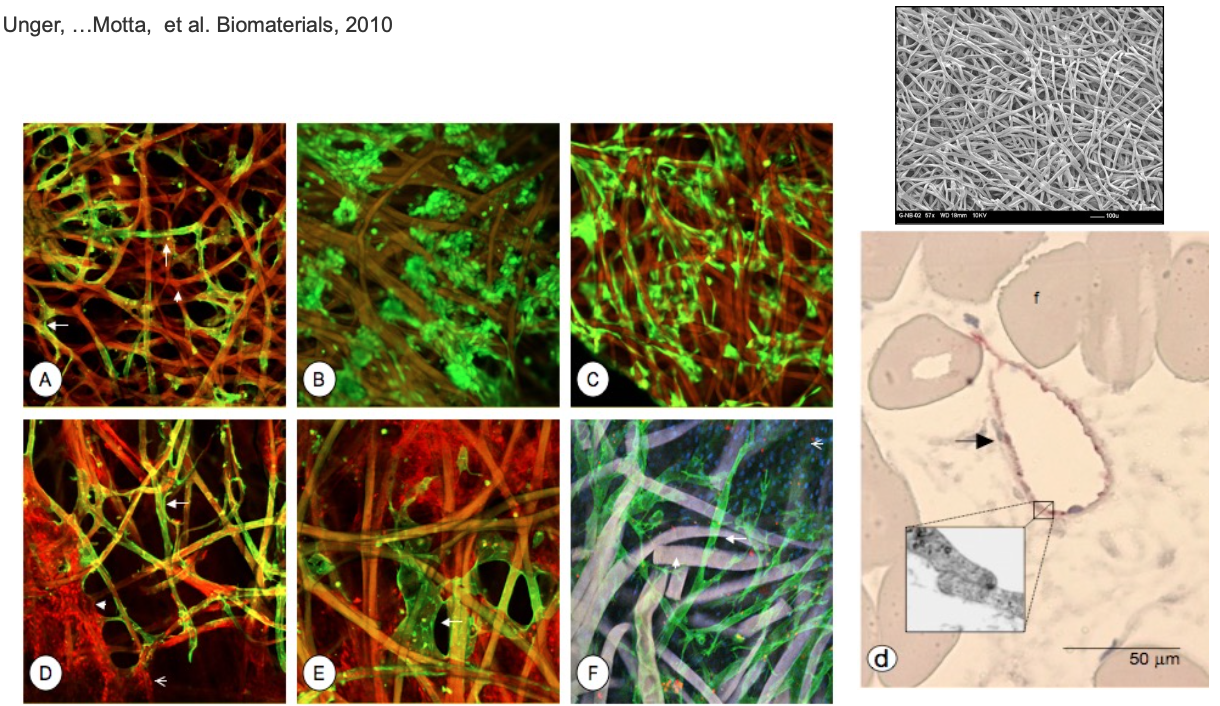
\includegraphics[width=0.5\textwidth]{fibroin}
            \caption{\label{fig:fibroin}}
        \end{figure}

        Figure \ref{fig:fibroin} represent a fibroin micronet with human microcapillary endothelial cells (HDMEC) and primary human osteoblast cells (HOS) left in co-culture for 10 days.
        The images show good result: the tubes are empty, but it is still promising.
        This tubes can be put into the scaffold and then maybe used as vessels.
        There is a need to check if the vessels connect to the circulatory system.

        \subsubsection{Pre-vascularized fibroin net}

        \begin{figure}[h]
            \centering
            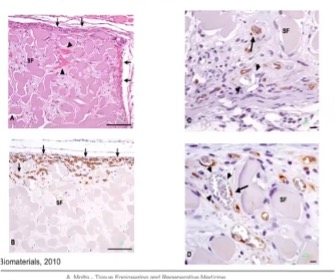
\includegraphics[width=0.5\textwidth]{osteoblast}
            \caption{\label{fig:osteoblast}}
        \end{figure}

        Figure \ref{fig:osteoblast} shows pre-vascularized fibroin net and in vivo anastomosis with host vasculature.
        Brown tubes are in vivo, and  blood cells are present and anastomise.
        The left image represent the scaffold loaded with osteoblast, incubated and then implanted.
        This shows fast angiogenesis, and only surface vessels.
        The right image represent the scaffold loaded with osteoblast and immediately implanted.
        In vitro human cells have been implanted in rat to identify the difference.
        On the right some capillaries that were produced can be seen and the absence of red blood cells can be noted.

        \subsubsection{Sponge formed from a NaCl solution}

        \begin{figure}[h]
            \centering
            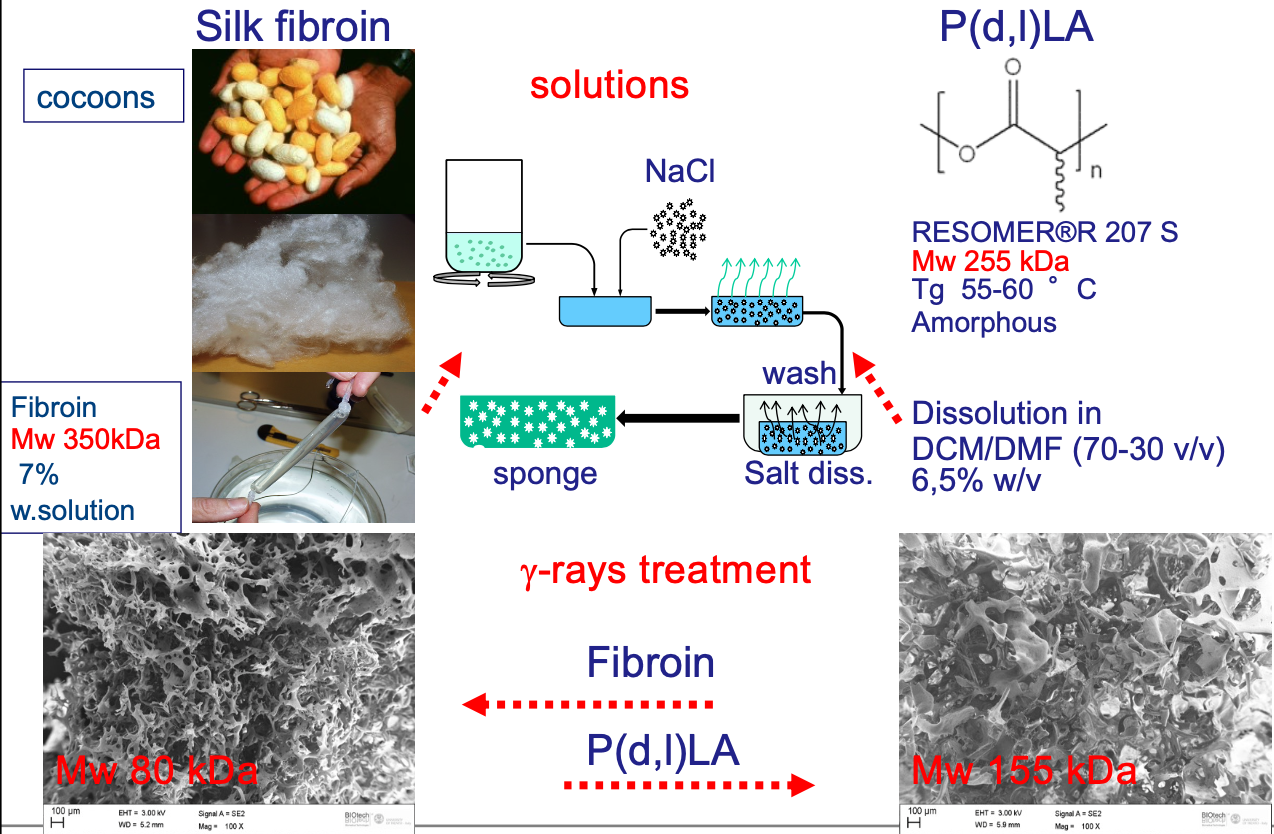
\includegraphics[width=0.5\textwidth]{salt}
            \caption{\label{fig:salt}}
        \end{figure}

        Figure \ref{fig:salt} depicts a sponge formed from salt crystals derived from a NaCl solution.
        The porosity depends on crystal size.
        Gamma rays treatment and add either silk fibroin or P(d,l)LA can be added.

        \subsubsection{Ectopic implant in rat}
        An ectopic implant is done in a sit that is not natural, in the studied case under the skin for bone.

        \begin{figure}[H]
            \centering
            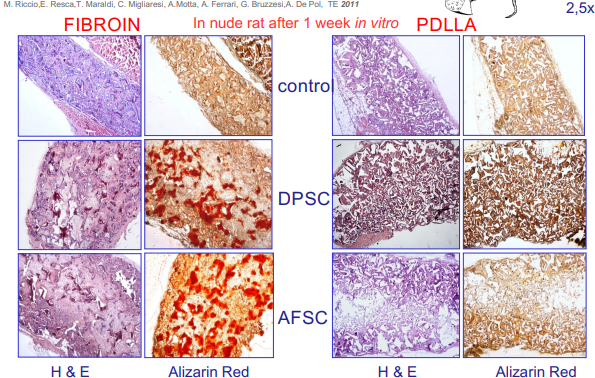
\includegraphics[width=0.5\textwidth]{implant_fibroin.png}
            \caption{\label{fig:implant_fibroin} \textbf{1. Fibroin.} In the \textbf{control} there is no red signal: no induction. There are cells (blue) but they are not infiltrated in the scaffold. There are no sign of mineralization. No osteoinduction. In \textbf{DPSC} and \textbf{AFSC} there are red nodules: it has become osteoinductive and force stem cells to become osteoblast and mineralization happens. In the H $\&$ E column a regeneration framework can be noted. \textbf{2. PDLLA} In the \textbf{control} there is not red sign so there is no induction. There are cells (blue) but they are not filtered in the scaffold. There is no mineralization or osteoinduction. In \textbf{DPSC} and \textbf{AFSC}, even in the case of pre-loaded cells there are no red signs and also there is no osteoinduction. In the center there are no cells and that suggests that the cells started to go into apoptosis.}
        \end{figure}

        \begin{figure}[H]
            \centering
            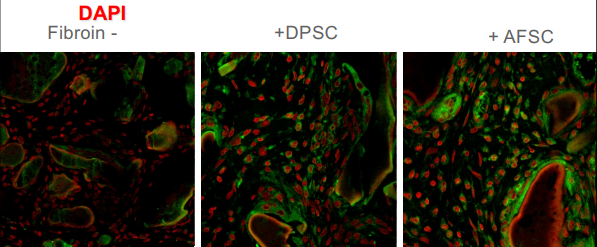
\includegraphics[width=0.5\textwidth]{fibroin_confocal.png}
            \caption{\label{fig:fibroin_confocal} In order to assess which kind of cell is working, pre-loaded cells or osteo-cells, anti-human staining can be performed.}
        \end{figure}

        \begin{figure}[H]
            \centering
            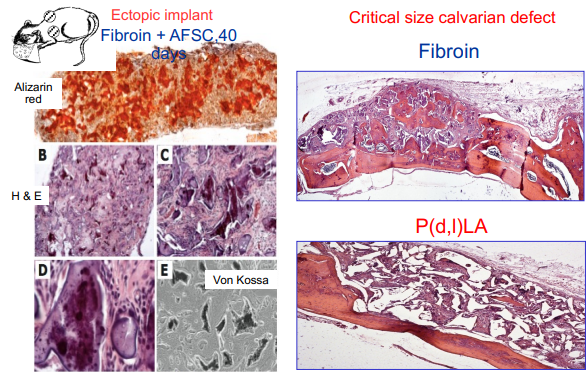
\includegraphics[width=0.5\textwidth]{intraosseous_implants.png}
            \caption{\label{fig:intraosseous_implants} \textbf{Intaosseous implants.} The \textbf{fibroin} enhance the new bone formation and supports regeneration. In \textbf{P(d,l)LA} there are lots of holes and the regenerations is not completed. It is possible to evaluate the quality of the bone and it can be seen in the fibroin it was good. There is a mixture of human and murine cells that are working together.}
        \end{figure}

        \begin{figure}[H]
            \centering
            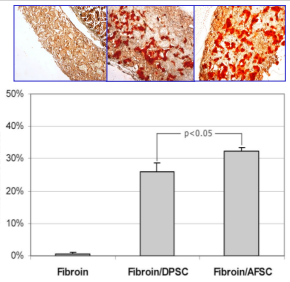
\includegraphics[width=0.5\textwidth]{mineralization.png}
            \caption{\label{fig:mineralization} \textbf{Areas of mineralization.} In the figure it is possible to see the areas of mineralization on fibroin scaffolds after 4 weeks implantation. It was calculated on 5 transversal sections cut at interval of 1 mm in the mid region of different fibroin stained by Alzarin Red. There is no mineralization in the scaffold with only fibroin, while there is mineralization in the two scaffold that present also AFSC and DPSC. There is no mineralization in the three scaffolds with PdILA.}
        \end{figure}


\section{Scaffold production technologies}

    \subsection{Cell sheet engineering}
    Cells sheet engineering is based on thermo-responsive polymers.
    They can be used in different sites like oral mucosa that present a very difficult regeneration, in periodontal ligament regeneration, but also in myocardium regeneration (as an alternative to heart transplantation).
    By transplanting single cell sheets directly to host tissues, skin, cornea, periodontal ligament, and bladder can be reconstructed.
    Additionally, the creation of co-cultured cell sheets from dishes with dual temperature-responsive domains, also allows for the re-creation of higher-order structures such as the kidney and liver.

    \begin{figure}[H]
            \centering
            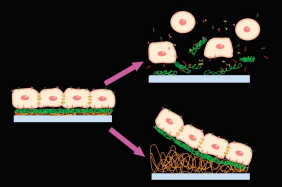
\includegraphics[width=0.5\textwidth]{cells_sheet1.png}
        \caption{\label{fig:cells_sheet1} Cell sheet harvest deposited ECM (green), as well as membrane proteins, so that confluent, monolayer cells are harvested as single cells (upper right). The temperature-responsive polymer (orange) covalently immobilized on the dish surface hydrates when the temperature is reduced, decreasing the interaction with deposited ECM. All the cells connected via cell-cell junction proteins are harvested as a single, contiguous cell sheet without the need for proteolytic enzymes.}
    \end{figure}

    \begin{figure}[H]
            \centering
            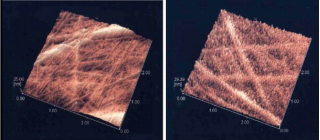
\includegraphics[width=0.5\textwidth]{cells_sheet2.png}
            \caption{\label{fig:cells_sheet2} Atomic force microscope images of temperature-responsive culture dish surfaces. Nongrafted, polystyrene culture dish surfaces (left) and poly(N-isopropylacrylamide)-grafted culture dish surfaces (right) were examined in air.}
    \end{figure}

    \begin{figure}[H]
            \centering
            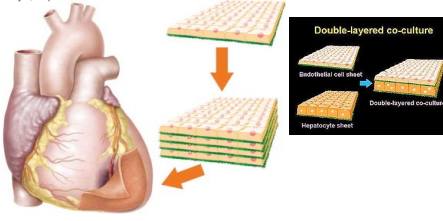
\includegraphics[width=0.5\textwidth]{cardiac_sheet.png}
            \caption{\label{fig:cardiac_sheet} Cardiac Tissue Reconstruction Based on Cell Sheet Engineering}
    \end{figure}

    \begin{figure}[H]
            \centering
            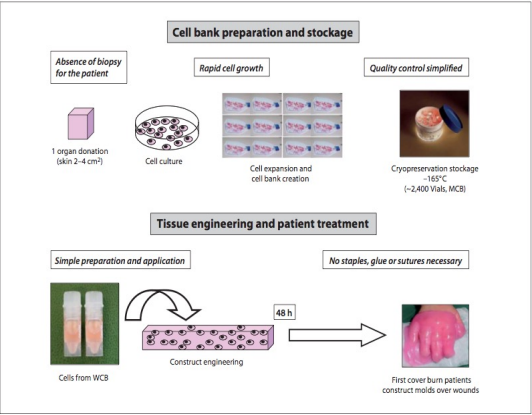
\includegraphics[width=0.5\textwidth]{cell_bank.png}
            \caption{\label{fig:cell_bank} Burnt skin}
    \end{figure}

        \subsubsection{Current challenges and strategies}

        \begin{figure}[H]
            \begin{multicols}{2}
                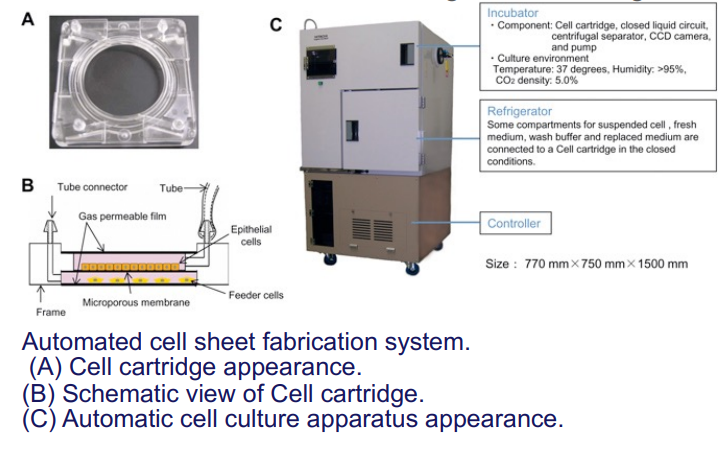
\includegraphics[width=0.5\textwidth]{strategies1.png}
                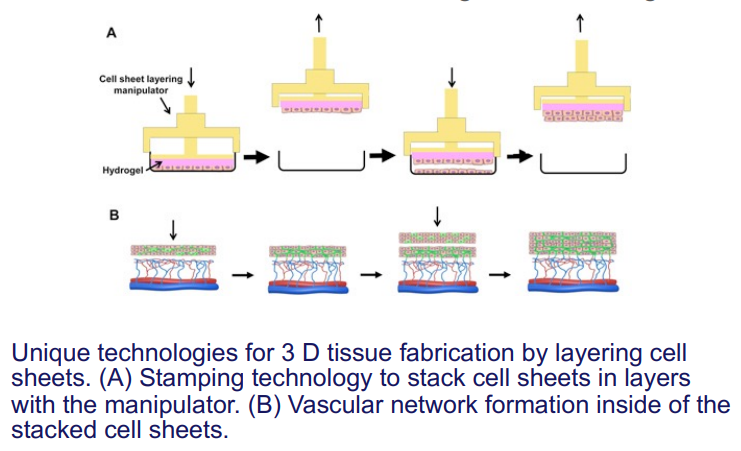
\includegraphics[width=0.5\textwidth]{strategies2.png}
                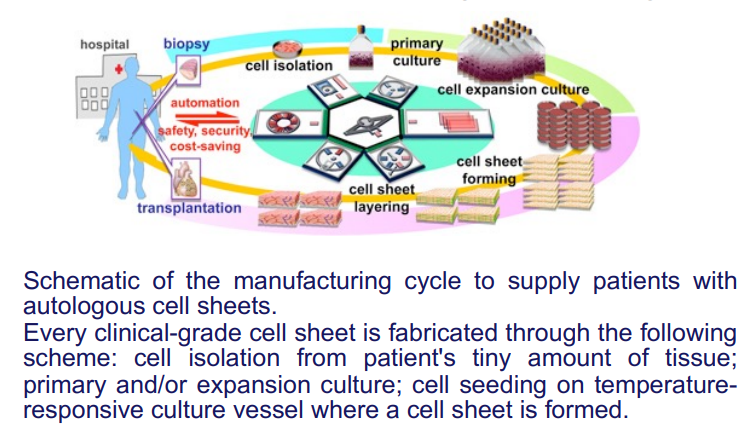
\includegraphics[width=0.5\textwidth]{strategies3.png}
                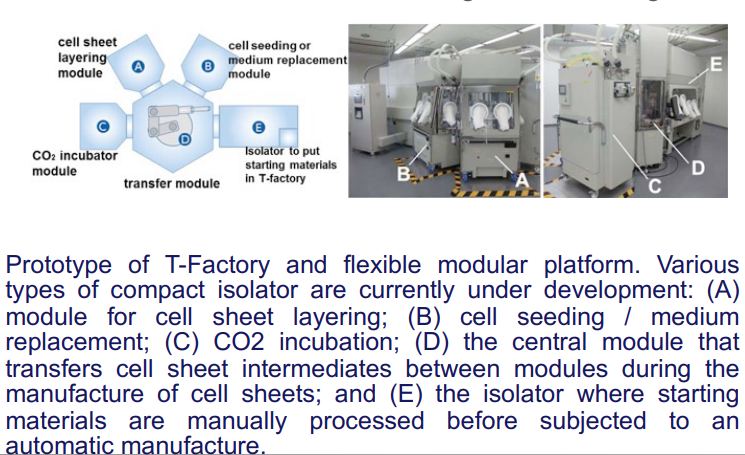
\includegraphics[width=0.5\textwidth]{strategies4.png}
            \end{multicols}
            \caption{\label{fig:strategies} Current challenges and strategies in cells sheet engineering.}
    \end{figure}

    \subsection{Cell encapsulation}
    The cell encapsulation methods consists in the entrapment of cells in microcapsules or microbeads starting from a suspension of cells in polymeric solution that can be solidified by chemical or physical methods.
    During the encapsulation the polymer cross-links by chemicals, magnetic field, light or by any other crosslinkers.

    \begin{figure}[H]
            \centering
            \includegraphics[width=0.5\textwidth]{encapsulation.png}
            \caption{\label{fig:encapsulation} (a) dropping the polyelectrolyte solution into a solution of small ions; (b) via a water in oil emulsification technique; and (c) complexation of oppositely charged polyelectrolytes by mixing, with additional coating procedures}.
    \end{figure}

        \subsubsection{Cell encapsulation requirements}
        Cell encapsulation requirements are:

        \begin{multicols}{2}
            \begin{itemize}
                \item The encapsulation material: a polymer should permit the free passage of nutrients and oxygen in and waste products out as well as of therapeutic protein products.
                \item Encapsulation material should prevent high Mw molecules, antibodies and other immunogenic moieties from contacting the encapsulated cells.
                \item The encapsulation material should protect cells from mechanical stresses and from the host's immune-response.
                \item The encapsulation material and method should not damage cells neither affect their behavior, as related to the desired function or application.
            \end{itemize}
        \end{multicols}

        \subsubsection{Cell encapuslation applications}
        Possible applications for cells encapsulation are drug delivery, bioartifical organs and tissue engineering.

        \begin{multicols}{2}
            \begin{itemize}
                \item The encapsulation of therapeutic cells permits the implantation of allogenic and xenogenic cells for the regulation of certain physiological processes damaged by death or senescence of host tissues.
                \item Microcapsules injected at the transplantation bed allow the release of biomolecules produced by the encapsulated cells, such as insulin produced by encapsulated $\beta$-cells for diabetes type I therapy, pro-angiogenic or anti-angiogenic growth factors to enhance or inhibit vascularization.
                \item Microencapsulated cells can be used as building blocks for the fabrication of tissues-tissue precursor in vitro or implanted in vivo for tissue regeneration.
            \end{itemize}
        \end{multicols}

\subsubsection{Short-term encapsulation effects}

\begin{figure}[H]
        \centering
        \includegraphics[width=0.5\textwidth]{short_term.png}
        \caption{\label{fig:short_term}}
\end{figure}

Short-term encapsulation effects include:

\begin{multicols}{2}
    \begin{itemize}
        \item The main function of HSP proteins consist in cells protection against apoptosis, necrosis, hypoxia or any other type of stress.
        \item Elevated co-erexpression of HSP70B' and caspase-3 genes points to mild stress conditions, and cells protection activity.
        \item The results were supported with Live/Dead test, where we can observed cell death within 48 hours after encapsulation
    \end{itemize}
\end{multicols}

\subsection{Electro-hydrodynamic jetting (EHDJ)}
In the electro-hydrodynamic systems a solution is fed through a positively charged metallic needle.
The solution reacts to the presence of the charge, generating repulsive coulombic forces on its surfaces, causing the deformation of the meniscus at the tip of the needle into a Taylor cone.
If the voltage is high enough, the electrostatic repulsion on the surface can overcome the surface tension at the apex of the liquid cone, leading to its disintegration (Rayleigh limit) and creating a jet of drops.
There are some parameters that we have to assess:

\begin{multicols}{2}
    \begin{itemize}
        \item Speed.
        \item Starting concentration of cells.
        \item Starting concentration of polymer.
        \item Type of polymer.
    \end{itemize}
\end{multicols}

Taking in consideration these parameters the final number outside of cells onto the beads can be controlled.
The quality of the concentration using a confocal microscope with live/dead staining \ref{fig:staining} can be controlled.
With this process is possible to check how many cells are alive and assess an optimal number of cells.

    \begin{figure}[H]
        \centering
        \includegraphics[width=0.5\textwidth]{staining.png}
        \caption{\label{fig:staining}}.
\end{figure}

    \graphicspath{{chapters/09/images/}}
\chapter{Vascularization}

\section{Angiogenesis and pore size}
Angiogenesis is the bottleneck of tissue engineering.
In order to regenerate functional tissues, stimulation, control or inhibition of angiogenesis are critical.
The porosity of the scaffold is fundamental for promoting vascularization.
A broad distribution of pore sizes and pore shapes ranging from very small to very large can be required.

	\subsection{A case regarding pore size}
	In fig \ref{fig:pores} is described the design of a very simple porous scaffold.
	This scaffold has been built combining polymers with spheres: holes filled with water and then emptied.
	The ratio between spheres and solution has to be tuned carefully.
	Black holes in the image are interconnections.
	Another technique to build such a scaffold is salt leaching, where we first add crystals to polymeric solution and then salt is removed.
	The regular shape is kept fixed thanks to crystal dimensions.
	In the case of spherical pores, the interconnection depends on the number of spheres per volume.
	Size and interconnection can be modulated by selecting the concentration.

	\begin{figure}[h]
		\centering
		\includegraphics[width=0.5\textwidth]{pores}
		\caption{\label{fig:pores}}
	\end{figure}

	The black dots representing interconnections have a dimension of $5$ micron.
	By playing with the scaffold, different families of pores can be obtained.
	In the case of smaller pores more capillaries are obtained.
	The ideal range for the black dots is between 40 and 50 microns.
	The highest vascular density was observed in the case of smaller porosity, between 0 and 100 micrometers.
	Very large porosity leads to the formation of a layer of endothelial cell with no 3D tube required for vascularization.

\section{Scaffold vascularization strategies}
Different strategies can be employed to vascularize a scaffold.

	\subsection{Growth factor delivery}
	The delivery of single or multiple angiogenic GF to stimulate loading molecules can be performed by mixing with the polymer allowing for a fast release.
	To slow the release they can be included in a drug releasing system like polymeric nanoparticles.
	In this way the release of the factors will be tied with the degradation time of those nanoparticles.
	This factors can also be linked to the molecules to the polymeric chain.
	This strategies can be combined to allow for a sequential release of different factors.

	\subsection{Cell transplantation}
	In cell transplantation cells and extracellular matrix are grown outside the body and then implanted to promote vascularization.

	\subsection{Scaffold pre-vascularization}
	Robust tubes in the scaffold are produced in order to anastomize with osteoblasts.
	Factors to attract already existing vascular tubes to the scaffold can be used.

	\subsection{Decellularized  scaffold}
	A human derived, decellularized myocardium not populated by endothelial cells is used to promote vascularization.
	The main difficulty in this strategy is to guarantee a very low amount of DNA.
	There is a need to check that no debris is left after decellularization to avoid thrombogenesis through forced migration to reform endothelium.

	\subsection{Angiogenic biomaterial}
	An angiogenic biomaterial is the best option if possible.
	The biomaterial is designed such that it is able to induce vascularization per se.
	These are called “precision biomaterials”, as they are designed to have a specific function.
	They can be nature derived biomaterial like proteins derived from silk that have intrinsic angiogenic potential or synthetic functionalized biomaterials.

	\subsection{Microfabrication methods}
	Microfabrication methods are a top-down approach: they built the vessels and around them the tissue.
	Decellulariziation can be skipped by directly inserting endothelial cells.

\section{Angiogenic potential evaluations}
In vitro procedures should be carefully designed, to obtain useful considerations on the scaffold.
Consider figure \ref{fig:coculture}: mononuclear cells are seeded inside the hydrogel upon isolation of two main endothelial progenitor cells populations from peripheral blood.
Cells were seeded and checked after 4 and 10 days.
In the case of IKVAV modified culture there is more signals.
This means there are more cells, more clusters and more layers due to migration.
The aim was to design a precision material to be used in brain, laminin derived to mimic the brain ECM.
The strategy consisted of isolation of peptides involved in differentiation and linking them to polymeric chain.
During angiogenesis tubes are expected to form, but this didn't happened, because the in vitro model was too far from physiology: the cell are not in a monolayer.
Changing the model cells were able to drive tube formation.

\begin{figure}[h]
	\centering
	\includegraphics[width=0.5\textwidth]{coculture}
	\caption{\label{fig:coculture}}
\end{figure}

	\subsection{Stem cells}
	In studies concerning donor-derived stem cells at least $5$ replicates need to be used.
	The personalized solution in order to avoid variability is needed to achieve the best result.

	\subsection{Bone scaffold}
	Considering bone, the presence of two families of cells leads to the best results: osteoblast work will lead to an increase endothelial cells formation.
	This is because osteoblast cells know how much and when to release factors.
	Osteoblasts also produce a collagenic template used by endothelial cells to form tubes.
	When we take into account the scaffold, the direct interaction with both osteoblast and endothelial cells using for example fibroin micronets.
	The endothelial cells become tubes creating a collagenic network.

\section{Vascularization strategies}
To achieve better blood vessels architecture is important.
Endothelial cells must be fed with some molecules to amplify the angiogenesis process.
Porous matrices can be loaded with growth factor and functionalized to recruit blood vessels from surrounding tissues.
They should be able to penetrate and form interconnected tissue.
The main vascularization strategies are:

\begin{multicols}{2}
	\begin{itemize}
		\item Angiogenesis: ingrowth of vascular sprouts from the host microvasculature into implanted tissue construct, which finally form a new microvascular network.
		\item Inosculation: a pre-created vessels in vitro is generated within a tissue construct prior to implantation.
			Then a connection with host vessels and already included vessels happens.
			Usually animal cells are used in order to distinguish which vessels are new and which are implanted through staining.
			Sometimes scaffold tubes are not able to anastomize and die, the aim is to preserve the mixture and anastomize.
	\end{itemize}
\end{multicols}

\begin{figure}[h]
\centering
\includegraphics[width=0.3\textwidth]{vasc}
\caption{\label{fig:vasc}}
\end{figure}

	\subsection{Immune response and vascularization}
	Inflammation induces angiogenesis.
	After the recruitment of macrophages and the formation of granulation tissue this must be vascolarized.
	In the case of a high porosity structure a fine granulation tissue is found, with the presence of angiogenic factors and new vessels.
	After $2$ week the inflammatory response ha decreased.
	In the case of a less porous scaffold there is no vascularization and a thick layer of fibrotic tissue.

	\subsection{Effect of silk fibroin on vascularization}
	So, to promote vascularization the polymer should form a sponge, like:

	\begin{multicols}{2}
		\begin{itemize}
			\item PDLLA: blood vessels are just around after $3$ weeks.
			\item PDLLAA and silk fibers: there is a very nice capillary branch formation into the scaffold after $3$ weeks.
		\end{itemize}
	\end{multicols}

	After 6 weeks silk seems to be intrinsically angiogenic.
	The best scaffold will always be the one with the quickest angiogenesis.

	\begin{figure}[h]
		\centering
		\includegraphics[width=0.5\textwidth]{pdlla}
		\caption{\label{fig:pdlla}}
	\end{figure}


	\subsection{Angiogenesis driven by inflammatory cells}
	In this experiment the fibroin net was implanted with and without pre-seeding osteoblasts.
	A very nice and intense angiogenesis was observes thanks to the interaction between osteoblasts and inflammatory signal.
	Different pre-culture time show that the inflammatory response better in the case B.
	The second scaffold has a better angiogenesis.
	Because of this it can be said that the drug release system works and speeds up the angiogenesis process.

	\begin{figure}[h]
		\centering
		\includegraphics[width=0.5\textwidth]{fibroin}
		\caption{\label{fig:fibroin}}
	\end{figure}

\section{Induction of vascularization in TE scaffolds}
After the selection and dosage of the molecules necessary to promote angiogenesis how to release them into the system must be decided.

	\subsection{PDGF-containing microspheres}
	A dual factor delivery from degradable scaffolds for de novo blood vessels synthesis can use PDGF-containing microspheres.
	The molecules must exit from the vescicles, move in a matrix and then release in a very slow process.
	The fact that degradation does not occur prior to release and wheter microparticles are active and alive throughout the waiting needs to be assessed.

	\subsection{Cytokine delivery}
	The sequential delivery of VEGF and PDGF-BB using a controlled release polymeric device subcutaneously and in hind limb ischemia model induced a mature new vascular network with vessels having a thick coat of smoot muscle cells.
	The combination of the two gives the best and fastest angiogenesis.

	\subsection{Microparticles}
	Scaffold design by microparticle assembly.
	Microparticles preparation:

	\begin{multicols}{2}
		\begin{itemize}
			\item Formation of microparticles via single emulsion.
			\item Double emulsion with growth factors.
		\end{itemize}
	\end{multicols}

	This methods includes microspheres loaded or not with drugs.

		\subsubsection{Sintering}
		Sintering is the formation of microparticles with some porosity inside.
		Single emulsion is a method of sintering.
		The sintering process allows for a good adhesion.
		It is usually used for metallic-alloy, polymers and ceramics.
		The porosity can be controlled by mixing the solution iwth water.

		\subsubsection{Printing}
		Microparticles are printed.

	\subsection{Strategies for enhancing vascularization}

	\begin{table}[H]
		\centering
		\begin{tabular}{|c|c|c|}
			\hline
			& By host & Engineered vascular network\\
			\hline
			\multirow{2}{*}{Pros} & Easy to engineer & Immediate perfusion\\
														& High quality vessels &\\
			\hline
			\multirow{3}{*}{Cons} & Too slow & Hard to engineer\\
														& 				 & Compatibility\\
														& 				 & Needs tubes\\
			\hline
		\end{tabular}
		\caption{Pros and cons of strategies for enhancing vascularization}
	\end{table}

    \graphicspath{{chapters/10/images/}}
\chapter{Bioreactors}

\section{Scaffold development process}
We start from a pathology, analyze the microenvironment (not only chemical signals, but also mechanical signals and the ability to heal) and the tissue to regenerate. 
From this info we can build a scaffold able to mimic the original biological morphology. 
The goal must be reached by carefully designing materials and manufacturing methods. 
E.g. 3D printing layer by layer allows us to build gradients with different properties. 
After obtaining a scaffold, we need to characterize it with biological function. 
Once a good result is obtained ,we can pass to clinical trials: first of all we need to make sure that we are not producing damages to the body, secondly it is required to demonstrate the suitability for therapeutic purposes.

\section{3D structures}
Growing cells on flat surfaces is unnatural and artificial, it does not make sense in a biological perspective.
Natural ECM plays an important role in regulating cellular behaviours by influencing cells with biochemical signals and topographical cues.
In 3D cultures, we can control scaffold morphology, architecture and chemistry, bio recognition signaling, degradation mechanisms, patterns; cells behave and respond to stimuli more like they would do in vivo.
\\
\\
\noindent
2D culture substrates are not able to reproduce the complex and dynamic environments of the body, forcing cells to adjust to an artificial flat, rigid surface. 
3D matrices or scaffolds are porous substrates that can support cell growth, organisation, and differentiation on or within their structure. 
Architectural and material diversity have much more impact on 3D matrices than on 2D substrates. 
Chemical and biochemical modification with specific biological motives can be added to facilitate cell adhesion, cell mediated proteolytic degradation and growth factor binding and release. 
\\
\\
\noindent
In order to build an effective scaffold we must be very precise and stick to biological processes.  
While working in vitro, we must carefully choose cells e.g. monocytes to evaluate immune response. 
The mechanics should be dynamic, not static. 
We need to decide stresses to apply, their intensity and timing. 
Bioreactors should always be designed by keeping in mind the application.

\section{Biomimetic approach}
In order to engineer matrices, we need to start from a reliable biological model. 
Matrices contain some factors that are able to induce specific cellular behaviours e.g. speed up regeneration, drive the healing process. 
The best way to engineer a tissue is through the biomimetic approach i.e. mimic the main aspects of the biological material by isolating specific signals. 
\\
\\
\noindent
Pharmaceutical industries are looking for trustful models with the purpose of evaluating the impact of a drug. 
3D tissue development allows us to exploit cancer tissues e.g. high patient variability in cancer can be overcome by building a patient-specific model. 

\section{3D culture engineering}
We start from stem cells and a scaffold, culture in bioreactor and check whether stem cells differentiate in the desired phenotype.  
\\
\\
\noindent
Challenges:
\begin{itemize}
\item how many cells are needed to replace normal function?
\item in vitro tests must be carefully designed to recapitulate nutritional requirements, structural needs, mechanical support and shear stress
\item Design a large scale industry product. We need to take into account complexity, time for production and cost. Reproducibility must be guaranteed, as well as sterilization and eventual parameters that can be modified.
\end{itemize}

\section{In vitro testing}
Before moving to animal models, we should check in vitro the cell/tissue responses.
We can use different instruments, among which imaging is the most popular. 
Furthermore, we can perform immune staining for molecules, receptors, etc.

\subsection{Mechanical stress}
Matrix elasticity/stiffness is very relevant in inducing specific behaviours in stem cells. 
The lowest stiffness is required for adipocytes, highest for bone. 
\begin{itemize}
\item shear stress e.g. endothelium: blood flow
\item compression e.g. cartilage
\item hydrostatic pressure e.g. chrondrcytes
\item tensions e.g. tendons
\end{itemize}
In all cases we also need to define the strength, time etc.

\subsection{Morphology}
\begin{itemize}
\item roughness e.g. modulation in phenotype of osteoblasts in permanent prosthasis
\item random features
\item anisotropic features
\item isotropic features
\end{itemize}

\section{Case of study}
Soluble signalling molecules in cartilage collagenic structures differ,  we have  an intermediate transition zone and bone. 
We can induce cartilage regeneration (difficult due to lack of vascularization) by injecting adipose derived stem cells into microspheres. Two types of microspheres should be employed,  as two different signals are required to control timing. 
In this case the patient is the bioreactor.
The polymer is sensible to UV light for polymerization. 
The irradiation should be safe for cells, we need to require a specific intensity. 
Furthermore, the irradiation should be really focused on the polymeric matrix. 

\section{Mathematical modelling of 3D cultures}
We need to define computational approaches and in silico models to carefully evaluate parameters. Furthermore, cell growth and migration can be modelled.

\section{Bioreactors}
Bioreactors need to be changed according to specific applications e.g. 3d print scaffold directly inside the bioreactor. 
A bioreactor is composed by a chamber containing cells and an in and out circulation system (to remove and add culture medium).
New ones can have sensors for level of oxygen, the production of specific molecules etc.
Mechanical stresses are induced e.g. medium circulation or rotation(shear stress movement).
Bioreactors can be used for large scale cell cultivation e.g. genetically modified bacteria for cellulose production.  A bioreactor should provide efficient mass transfer through the scaffold, precise spatial distribution of cells in 3D and expose tissue to physical stimuli. 
The bioreactor is responsible for the environment control, nutrient delivery and mechanical stimulation.







\end{document}
